\section{几何域：5G}


%As already mentioned, the geometric priors of symmetry and scale separation can be instantiated across a broad range of geometric domains of increasing level of specialization. 
%
%Since the subtitle of our book is `4G', 

本文将重点讨论图、网格、群、测地线和规范。在这里，“群”是指齐性空间中的全局对称变换，“测地线”是指流形上的度量结构，而“规范”是指定义在切丛（以及一般向量丛）上的局部参考标架。
后文将更详细地解释这些概念。
%\marginnote{A {\em gauge} is a choice of frame (system of coordinates) for a collection of vector spaces attached to some base manifold, such as the tangent space to a manifold, or an RGB color vector attached to each position in a planar image. This term is used in physics. 
%}, and . % where `gauges' is a high-energy physics parlance for objects with manifold structure. 
%where grids can be considered 
%
%In this Section we introduce the main geometric domains 
%that will be the central focus of the book: Graphs, Grids, Gauges and Groups, 
%
在接下来的各节中，我们将详细讨论这些结构的主要共同要素与关键区别，并描述与之相关的对称群。
%
本文并不按普适性顺序展开——事实上，网格是图的特例——而是力求突出几何深度学习蓝图背后的重要概念。




\begin{figure}
    \centering
    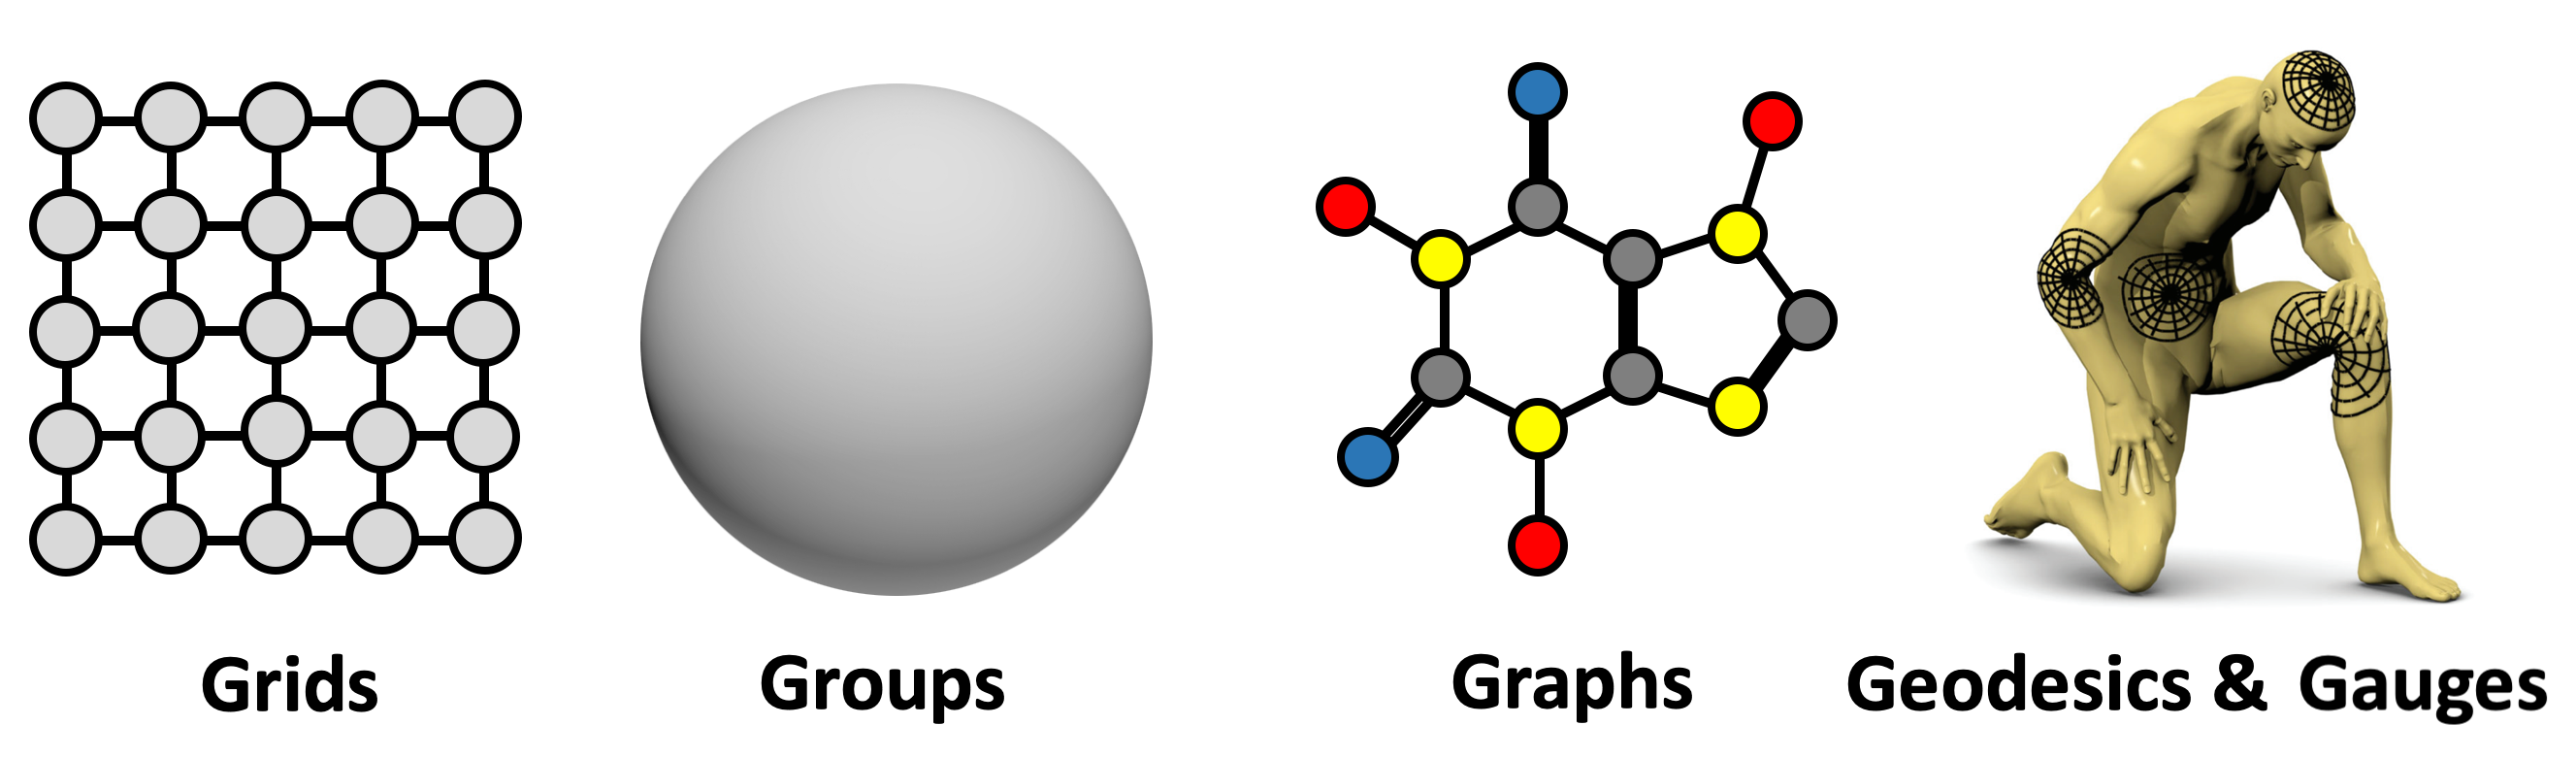
\includegraphics[width=1\textwidth]{figures/5g.png}
    \caption{几何深度学习的 5G：网格，具有全局对称性的群与齐性空间，图，流形上的测地线与度量，以及规范（切空间或特征空间的标架）。}
    \label{fig:4g}
\end{figure}





\subsection{图与集合}\label{sec:proto-graphs}

%\joan{This is a very nice intro. 
%Just one comment: it would be great to use the transition from sets to graphs to reinforce the scale aspect mentioned in the previous sections. Sets cannot be coarsened in non-trivial ways, while graphs can. 

%Another more general aspect that we need to nail in this section that clearly separates the graph treatment from, say the grid treatment: the domain varies with the input and thus becomes `part' of the input. I think again the transition from set to graph is useful here. The set is always the same geometric object modulo the change in size. The graph provides a new input to the system (as you say, via et its adjacency). 
%}





%\michael{\bf [MB: I took the liberty to rewrite this section making it less detailed and more `conversational' like the style of the previous sections in the Introduction chapter, anticipating that Chapter on graphs to be more rigorous.]}


%\joan{Joan: 
% Great detail and everything important seems to be here already. Two remarks:
% \begin{itemize}
%     \item I would frontload the section a bit more, explaining that we will first describe the domain, and then explain how the geometric priors and the blueprint are expressed.
%     \item Currently, this section re-derives the definitions of invariance/equivariance described previously, as well as the blueprint. I think it can be made shorter and more coherent to simply describe the two forms of group representation arising here (one for sets, and the other for graphs, where adjacency is also present), as well as the metric induced in the graph that is used to define local operators. 
%     \item In other words, I think these sections should derive the class of local linear equivariants for each symmetry group under consideration. In this section of sets and graphs, we should explain the two classes that arise (cf Maron et al.). 
%     \item The notation needs to be unified with the previous sections. 
%     
% \end{itemize}
%}

%\michael{MB: Agree in principle but we should not fall into the Bourbaki extreme. I suggest keep domain-specific notation to use familiar concepts and relate them to blueprint on the high level rather than in detail.

%I suggest to remove reference to particular models and talk about general concepts here. 
%}

在从社会学到粒子物理学的多个科学分支中，图都被用于对关系与交互系统建模。从我们的视角来看，图产生了一类由置换群刻画的基本不变性。
此外，我们关心的其他对象，如网格与集合，也可以作为图的特例得到。
%
%since graphs exhibit less restrictive geometries and invariances, they invite for the most flexible class of architectures---the \emph{Graph Neural Networks} (GNN). As we will see, all of the neural architectures we will study in this book can be understood as a special case of the GNN, with injected additional geometric constraints and invariances.


%the {\em symmetric group}), a . 


{\em 图} $\gG = (\gV, \gE)$ 由{\em 节点}\marginnote{视应用领域而定，节点也称为\emph{顶点}，边也常称为\emph{链接}或\emph{关系}。本文将交替使用这些术语。}集合 $\gV$ 以及节点对之间的{\em 边}集合 $\gE \subseteq \gV\times \gV$ 构成。为便于下文讨论，我们进一步假设节点配备 $s$ 维{\em 节点特征}，
记为 $\mathbf{x}_u$，其中 $u \in \gV$。
%
社交网络或许是最常研究的图实例之一，其中节点表示用户，边对应用户间的好友关系，节点特征则刻画年龄、头像等用户属性。通常也可以为边或整张图配备特征；\marginnote{
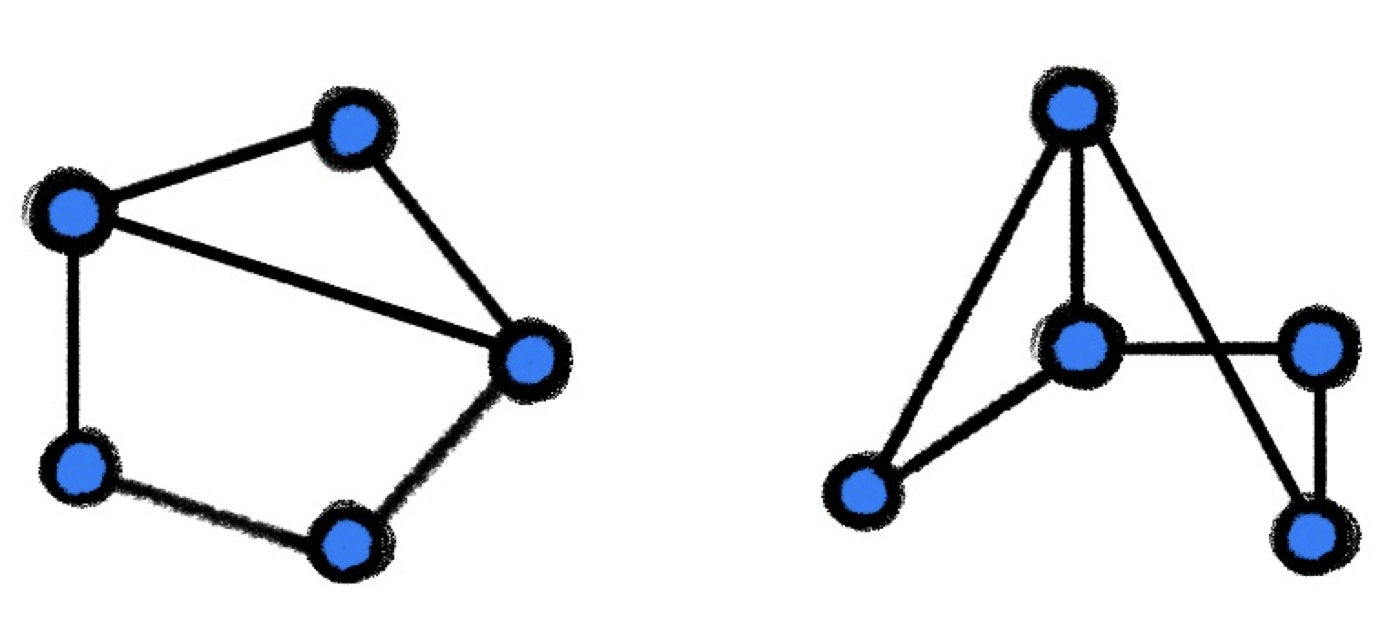
\includegraphics[width=0.8\linewidth]{figures/mn_isomorphic.png}
{\em 同构}是两个图之间保持边的双射。这里所示的两个同构图除节点顺序外完全相同。
}但这不会改变本节的主要结论，因此将留待后续工作讨论。


图的关键结构性质在于，通常不假设 $\gV$ 中的节点按任何特定顺序给出，因此在图上执行的任何运算都不应依赖节点排序。作用于图的函数所应满足的性质因而是{\em 置换不变性}；它意味着对于任意两个\emph{同构}图，这些函数的输出完全相同。
%
%
%This is clearly a 
我们可以把它视为蓝图的一种
特殊设定，其中域为 $\Omega = \mathcal{G}$，而空间 $\mathcal{X}(\mathcal{G},\mathbb{R}^d)$ 由 $d$ 维逐节点信号构成。
%
我们所考虑的对称性由\emph{置换群} $\mathfrak{G} = \Sigma_n$ 给出，其元素是节点索引集合 $\{1,\hdots, n\}$ 的所有可能排序。

%\michael{Harmonize notation: do we use $s$ or $d$ for dimension of features? } \joan{I am making a pass, using $s$ for feature dimension}\michael{we always used $d$, changing}

%In the language of the previous sections:\marginnote{However, we will almost always omit such notation for graphs, as they are assumed to be \emph{discrete} collections of nodes; hence, the language of linear algebra will admit higher notational simplicity.} for graphs we consider the input space to be defined on the domain  $\Omega = \mathcal{V}$, with the input space $\mathcal{X}(\mathcal{G}) = \{x : \mathcal{V}\rightarrow\mathbb{R}^s\}$ consisting of functions that attach node feature vectors to every node; $x(v) = \vec{x}_v$.
%\joan{Notation-wise: align with previous section $\Omega$ for domain, $\gX$ for signals over the domain} \michael{We use $x$ for signals, but $\Omega$ must be specific. }



%
%Accordingly, we focus on the permutation group actions $\frak{g}\in\frak{G}$ that permute the node ordering by applying such a matrix: $\frak{g}.{\bf X} = {\bf P}{\bf X}$. %


%$$ (where $n$ is the number of nodes).

%\begin{equation}
%    {\bf P}_{(2, 4, 1, 3)}{\bf X} =
%    \left[
%    \begin{array}{cccc}
%        0 & 1 & 0 & 0\\
%        0 & 0 & 0 & 1\\
%        1 & 0 & 0 & 0\\
%        0 & 0 & 1 & 0
%    \end{array}\right]\left[
%  \begin{array}{ccc}
%    \horzbar & \mathbf{x}_1 & \horzbar \\
%    \horzbar & \mathbf{x}_2 & \horzbar \\
%      \horzbar        &   \mathbf{x}_3  &    \horzbar       \\
%    \horzbar & \mathbf{x}_4 & \horzbar
%  \end{array}\right] = \left[\begin{array}{ccc}
%   \horzbar & \mathbf{x}_2 & \horzbar \\
%    \horzbar & \mathbf{x}_4 & \horzbar \\
 %     \horzbar        &   \mathbf{x}_1  &    \horzbar       \\
%    \horzbar & \mathbf{x}_3 & \horzbar
%  \end{array}\right]
%\end{equation}




%The first kind of object we will be studying is that of the \emph{graph}, which corresponds to the mother of all finite symmetry groups: the group of permutations. For the purposes of this chapter, we will define graphs as $G=(V, E)$, where $V$ is the set of \emph{nodes} and $E\subseteq V\times V$ is a set of \emph{edges} between pairs of nodes. For a commonly-studied example, social networks can be readily represented as graphs where nodes correspond to users, and edges correspond to the friendship links between them. 

%For now, we will assume that the graph's nodes are endowed with \emph{node features}, represented by $\mathcal{X} = \left\{\mathbf{x}_1, \mathbf{x}_2, \dots, \mathbf{x}_{|V|}\right\}$, where $\mathbf{x}_i\in\mathbb{R}^k$ are the features of node $i\in V$. In the social network analogy, these features could correspond to (some encoding of) the user's biography, interests or profile picture. Additional featurizations are possible, e.g. having features on the edges or entire graphs, but we will omit them for simplicity for now. 

%Compared with the subsequent objects, graphs exhibit less restrictive geometries and invariances, and hence invite for the most flexible class of architectures---the \emph{Graph Neural Networks} (GNN). Indeed, all of the neural architectures we will study can be understood as a special case of the GNN, with injected additional geometric constraints and invariances.

%The key structural property of graphs is that the nodes in $V$ are usually not assumed to be provided in any particular order, and thus any operations performed on graphs should not depend on the ordering of nodes. This desirable property that operations should satisfy is {\em permutation invariance}, and it implies that for any two \emph{isomorphic} graphs,\footnote{Isomorphism is an edge-preserving bijection between two graphs. Two isomorphic graphs are identical up to reordering of their nodes. } the outcomes of these operations are identical. 


首先在\emph{集合}上说明置换不变性的概念；集合是没有边的图的特例（即 $\gE=\emptyset$）。
%
将节点特征按行堆叠为 $n\times d$ 矩阵
 $\mathbf{X} = (\mathbf{x}_1, \hdots, \mathbf{x}_n)^\top$，实际上便指定了节点的一种排序。
 %
置换 $\mathfrak{g}\in\Sigma_n$ 在节点集合上的作用相当于重新排列 $\mathbf{X}$ 的各行；这一作用可以表示为一个 $n\times n$ {\em 置换矩阵} $\rho(\mathfrak{g}) = \mathbf{P}$，\marginnote{这样的置换恰有 $n!$ 个，因此 $\Sigma_n$ 即使在 $n$ 不大时也是一个非常大的群。}其中每行每列恰有一个 $1$，其余元素均为零。



%  We may obtain a different ordering by applying an appropriate permutation matrix  $\mathbf{P}$,\marginnote{There are exactly $n!$ such permutations. } where each row and column contains exactly one $1$ and all the other entries are zeros. Accordingly, we focus on the permutation group actions $\frak{g}\in\frak{G}$ that permute the node ordering by applying such a matrix: $\frak{g}.{\bf X} = {\bf P}{\bf X}$. %
 
 %\begin{equation}
 %    a(\vec{x}, \vec{y}) = \left<\vec{W}\vec{x}, \vec{U}\vec{y}\right> \qquad a(\vec{x}, \vec{y}) = \vec{a}^\top({\bf Wx} + {\bf Uy})
 %\end{equation}
 
 %\begin{align*}
 %    {\bf x}^\top{\bf L}{\bf x} &= \frac{1}{2}\sum_{u\in\mathcal{V}}\sum_{v\in\mathcal{V}} a_{uv}(x_u - x_v)^2\\ &= \sum_{(u, v)\in\mathcal{E}} (x_u - x_v)^2
 %\end{align*}

 
 %, ${\bf P}\in\mathbb{R}^{|V|\times|V|}$, to ${\bf X}$. 
 


%Let ${\bf X}\in\mathbb{R}^{|V|\times k}$ be a \emph{node feature matrix} which is obtained by stacking $\mathbf{x}_i$ in a particular order. This effectively specifies one \emph{ordering} of this set of node features; we may obtain any different order by applying an appropriate permutation matrix, ${\bf P}\in\mathbb{R}^{|V|\times|V|}$, to ${\bf X}$. 
若作用于该集合的函数 $f$ 对任意此类置换矩阵 ${\bf P}$ 都满足 $f({\bf P}{\bf X}) = f({\bf X})$，则称其具有\emph{置换不变性}。一个简单的此类函数是
%, exploited by the Deep Sets model \citep{zaheer2017deep}, is
\begin{equation}
\label{eq:basicinv}
    f({\bf X}) = \phi\left(\sum_{u\in \gV} \psi\left(\mathbf{ x}_u\right)\right)~,
\end{equation}
其中，函数 $\psi$ 独立地作用于每个节点的特征，$\phi$ 则作用于这些输出的\emph{求和聚合}结果。由于求和与输入的给定顺序无关，这类函数对节点集合的置换保持不变，因而无论如何置换节点，都保证返回相同的输出。

%\michael{Notation: should we use $\mathbf{f}(\mathbf{X})$ since the output can be a vector?}
%\petar{I would tend to stick with the $f$ notation}

 
%node features in $\mathcal{X}$ are permuted.



上述函数给出“全局”的图级输出，但很多时候，我们更关心以逐节点方式“局部”作用的函数。
%return more fine-grained information. 
例如，我们可能希望应用某个函数来\emph{更新}每个节点的特征，从而得到一组\emph{潜在}节点特征。
%, $\mathbf{h}_1, \hdots, \mathbf{h}_n$. 
%$\mathcal{H}=\left\{\mathbf{h}_1, \mathbf{h}_2, \dots, \mathbf{h}_{|V|}\right\}$.
%
%Strictly speaking, 
如果把这些潜在特征堆叠为矩阵 $\mathbf{H} = \mathbf{F}({\bf X})$\marginnote{我们对函数使用粗体记号 $\mathbf{F}(\mathbf{X})$，以强调它输出逐节点向量特征，因而是矩阵值函数。}，所得函数便不再具有置换不变性：${\bf H}$ 的行顺序应与 ${\bf X}$ 的行顺序\emph{绑定}，这样才能知道哪个输出节点特征对应哪个输入节点。我们转而需要更细致的{\em 置换等变性}概念：一旦“选定”输入的一种置换，该置换就会一致地作用于所得对象。
%
形式化地说，若 $\mathbf{F}(\mathbf{X})$ 对任意置换矩阵 ${\bf P}$ 都满足 $\mathbf{F}({\bf P}{\bf X}) = {\bf P}\mathbf{F}({\bf X})$，则它是\emph{置换等变}函数。一个共享的逐节点线性变换
\begin{equation}
    \mathbf{F}_{\mathbf\Theta}({\bf X}) = {\bf X}{\mathbf \Theta}
    %\qquad \text{, i.e.,} \qquad {\vec h}_i = {\mathbf\Theta}^T\mathbf{x}_i
\end{equation}
由权重矩阵 $\mathbf\Theta\in\mathbb{R}^{d\times d'}$ 指定，是构造此类置换等变函数的一种方式；在我们的例子中，它产生如下形式的
潜在特征：
$\mathbf{h}_u = \boldsymbol{\Theta}^\top\mathbf{x}_u$.
%\joan{This is very clear and nicely explained, but it is a particular case of the group equivariance discussion from previous section. I would add a pointer at the beginning or the end of this paragraph to tie things together. Upps just saw the following paragraph, nevermind. }

%\michael{Notation: do we use $h$ or $y$ for output?}
%\petar{$h$ for what comes out of an equivariant layer; the assumption is that we can stack more than one, or even attach invariant tail, to get a desirable $y$ (which should maybe be reserved for downstream task outputs?).}


%In fact, the construction from Equation (\ref{eq:basicinv}) arises naturally from the GDL blueprint. 
这一构造自然地源自几何深度学习蓝图。
我们可以首先尝试刻画{\em 线性等变映射}（形如 $\mathbf{F} {\bf P X} = \bf{P} \mathbf{FX}$ 的函数）；容易验证，
任意此类映射都可以写成两个\emph{生成元}的线性组合：恒等映射 $\mathbf{F}_1 \mathbf{X} = {\bf X}$ 与平均映射 ${\mathbf{F}_2 \mathbf{X}}= \frac{1}{n}\boldsymbol{1}\boldsymbol{1}^\top \mathbf{X} = \frac{1}{n} \sum_{u=1}^n {\bf x}_u$。正如第~\ref{sec:deepset} 节将描述的，流行的 Deep Sets \citep{zaheer2017deep} 架构恰好遵循这一蓝图。
%\joan{Remark to avoid confusion that $\mathbf{X}$ here should be understood as a vector, not a matrix}


% TODO: explain relation to representations & equivariance as explained in previous section.
% Invariant features correspond to a trivial representation
% Node features correspond to rho(P) = P
% Edge features / adjacency matrix corresponds to rho(P) = P tensor P.


现在可以把置换不变性与等变性的概念从集合推广到图。
%
在一般设定 $\gE\neq\emptyset$ 下，图的连通性可由如下定义的 $n\times n$ {\em 邻接矩阵} $\mathbf{A}$ 表示，\marginnote{当图为{\em 无向图}时，即 $(u,v) \in \gE$ 当且仅当 $(v,u) \in \gE$，邻接矩阵是{\em 对称的}：$\mathbf{A}= \mathbf{A}^\top$。}
\begin{equation}
    a_{uv} = \begin{cases}
    1 & (u, v)\in \gE\\
    0 & \text{otherwise}.
    \end{cases}
\end{equation}
%
注意，此时邻接矩阵 $\mathbf{A}$ 与特征矩阵 $\mathbf{X}$ 是“同步的”，即 $a_{uv}$ 指定了由第 $u$ 行和第 $v$ 行所描述节点之间的邻接信息，而这些行属于 $\mathbf{X}$。因此，把置换矩阵 $\mathbf{P}$ 施加于节点特征 $\mathbf{X}$，就必然也要对 $\mathbf{A}$ 的行和列施加置换，得到 $\mathbf{P}\mathbf{A}\mathbf{P}^\top$。\marginnote{$\mathbf{P}\mathbf{A}\mathbf{P}^\top$ 是 $\Sigma_n$ 作用于矩阵的表示。}
%
%
若（图级函数）$f$ 满足下式，则称其具有\emph{置换不变性}：
\begin{equation}
f({\bf PX}, {\bf PAP}^\top) = f({\bf X}, {\bf A})\marginnote{As a way to emphasise the fact that our functions operating over graphs now need to take into account the adjacency information, we use the notation $f({\bf X}, {\bf A})$.}
\end{equation}
若（逐节点函数）$\mathbf{F}$ 满足下式，则称其具有\emph{置换等变性}：
\begin{equation}
\label{eq:permequivgraph}
\mathbf{F}({\bf PX}, {\bf PAP}^\top) = {\bf P}\mathbf{F}({\bf X}, {\bf A})
\end{equation}
其中 ${\bf P}$ 为任意置换矩阵。
%
%
%\taco{Taco: should we relate this to the blueprint? We can mention here that $PX$ and $PAP^T$ are examples of representations of the permutation group. We can then go on to say that the graph structure tells us which nodes are close in a certain sense, and that most graph nets exploit this, leading into the next paragraph.}\michael{I do say above that $\rho(\fg)=P$}
%
%Armed with the concepts of permutation invariance and equivariance, we can consider a generic graph connectivity setup, where $E\neq\emptyset$. One typical way to represent this adjacency information in a compact form is the \emph{adjacency matrix}, ${\bf A}\in\mathbb{R}^{|V|\times|V|}$, which is in the simplest case (of an unweighted and undirected graph), a binary and symmetric matrix; that is:
%\begin{equation}
%    {\bf A}_{ij} = {\bf A}_{ji} = \begin{cases}
%    1 & (i, j)\in E\\
%    0 & \text{otherwise}
%    \end{cases}
%\end{equation}
%
%
%We can now generalise the notions of permutation invariance and equivariance from sets to graphs. We note that the order of the rows and columns in ${\bf A}$ is constrained to respect the order of the rows of ${\bf X}$---that is, ${\bf A}_{ij}$ specifies the adjacency information between the nodes described by the $i$-th and $j$-th row of ${\bf X}$. Then, applying a permutation matrix ${\bf P}$ to the nodes in ${\bf X}$ automatically implies applying it to ${\bf A}$'s rows and columns, yielding ${\bf P}{\bf A}{\bf P}^T$. 


%Following again the Geometric Deep Learning blueprint, 
这里同样可以先刻画线性等变函数。\marginnote{这对应于{\em Bell 数} $B_4$，它计算对含 $4$ 个元素的集合进行划分的方式数；此处这四个元素是为作用于邻接矩阵的线性映射编制索引的四个指标 $(u,v), (u',v')$。%\cite{maron2018invariant}.
}  
正如 \cite{maron2018invariant} 所观察到的，任何满足式（\ref{eq:permequivgraph}）的线性 $\mathbf{F}$ 都可以表示为
十五个线性生成元的线性组合；值得注意的是，这一生成元族与 $n$ {\em 无关}。
%
%
%
在这些生成元中，我们的蓝图尤其提倡同时具有{\em 局部性}的生成元，即
节点 $u$ 上的输出直接依赖图中与其相邻的节点。通过定义一个节点与另一个节点相邻的含义，可以在模型构造中显式形式化这一约束。



节点 $u$ 的（无向）{\em 邻域}有时也称为 {\em 1-hop}，定义如下：\marginnote{
%Our definition of neighbourhood does not account for directed edges. 
通常也把节点 $u$ 本身包含在其邻域中。}
\begin{equation}
    \mathcal{N}_u = \{ v : (u,v) \in \gE \,\mathrm{or}\, (v,u) \in \gE \}
    %\left\{j\ |\ i=j\vee {\bf A}_{ij} = 1\right\}
\end{equation}
%
并把{\em 邻域特征}定义为多重集
%
\begin{equation}
    \mathbf{X}_{\mathcal{N}_u} = \ldblbrace \mathbf{x}_v : v\in\mathcal{N}_u \rdblbrace.
\marginnote{A {\em multiset}, denoted $\ldblbrace \, \dots \, \rdblbrace$, is a set where the same element can appear more than once. This is the case here because the features of different nodes can be equal.}
\end{equation}
%%
对 1-hop 邻域进行运算与蓝图的\emph{局部性}方面非常契合：具体而言，把图上的度量定义为沿 $\mathcal{E}$ 中边计算的节点间\emph{最短路径距离}。% \michael{I suggest we get rid of this, since we never talked about metrics in a rigorous way. } \petar{There seems to still be a discussion of a metric when defining locality in the blueprint---this is what I was referring to. I think it's fine as-is, but wouldn't mind removing it.} \joan{I think mentioning it qualitatively like this is fine, it conveys an important message}
%Processing 1-hop neighbourhoods over graphs exactly corresponds with defining our metric over graphs, $g$, as the \emph{shortest path distance} between nodes using edges in $\mathcal{E}$, and setting $\delta = 1$.

%This also closely aligns with the \emph{locality} condition of the main building block of our geometric deep learning blueprint. Processing 1-hop neighbourhoods over graphs exactly corresponds with defining our metric over graphs, $g$, as the \emph{shortest path distance} between nodes using edges in $\mathcal{E}$, and setting $\delta = 1$.

%
因此，GDL 蓝图给出了在图上构造置换等变函数的一般方案：指定一个作用于节点及其邻域特征的\emph{局部}函数 $\phi$，即 $\phi(\mathbf{x}_u, \mathbf{X}_{\mathcal{N}_u})$。随后，可以构造置换等变函数 $\mathbf{F}$，方法是把 $\phi$ 分别应用于每个节点的邻域（见图~\ref{fig:gc_gdl}）：
\begin{equation}
    \mathbf{F}({\bf X}, {\bf A}) =
\left[
  \begin{array}{ccc}
    \horzbar & \phi(\mathbf{x}_1, \mathbf{X}_{\mathcal{N}_1}) & \horzbar \\
    \horzbar & \phi(\mathbf{x}_2, \mathbf{X}_{\mathcal{N}_2}) & \horzbar \\
             & \vdots    &          \\
    \horzbar & \phi(\mathbf{x}_n, \mathbf{X}_{\mathcal{N}_n}) & \horzbar
  \end{array}
\right]
\label{eq:graph_equivariant}
\end{equation}
由于 $\mathbf{F}$ 是通过在每个节点处局部应用共享函数 $\phi$ 构造的，其置换等变性取决于 $\phi$ 的输出是否独立于 $\mathcal{N}_u$ 中节点的排序。因此，只要把 $\phi$ 构造为置换不变函数，就能满足这一性质。
%
正如后续工作将说明的，$\phi$ 的选择对这类方案的表达能力起着关键作用。当 $\phi$ 为单射时，它等价于{\em Weisfeiler-Lehman 图同构检验}的一步；这是图论中的经典算法，通过迭代颜色细化过程给出两个图同构的必要条件。


%\michael{ADD: geometric stability of graph filters}

%We conclude our introduction with a discussion on how to generally construct useful functions over graphs that are permutation equivariant. A function over graphs is likely to be useful if it directly exploits the structure present in ${\bf A}$---that is, if outputs on node $i$ directly depend on its \emph{neighbouring} nodes in the graph (e.g. the non-zero entries of $\mathbf{a}_i$ and $\mathbf{a}_i^T$).

%From this concept, we can define a \emph{neighbourhood} of node $i$ in the graph, commonly denoted as $\mathcal{N}_i$, to include all first-order neighbours of $i$, often including $i$ itself:
%\begin{equation}
%    \mathcal{N}_i = \left\{j\ |\ i=j\vee {\bf A}_{ij} = 1\right\}
%\end{equation}
%Accordingly, we can define the set of \emph{neighbourhood features} of $i$, $\mathbf{X}_{\mathcal{N}_i}\in\mathcal{P}(\mathbb{R}^k)$:
%\begin{equation}
%    \mathbf{X}_{\mathcal{N}_i} = \left\{\mathbf{x}_j\ |\ j\in\mathcal{N}_i\right\}
%\end{equation}
\begin{figure}
    \centering
    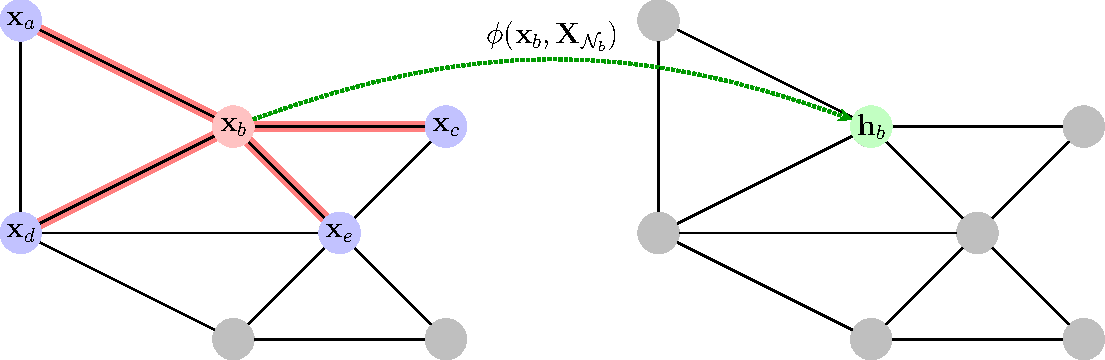
\includegraphics[width=\linewidth]{figures/GC_GDL.pdf}
    \caption{通过对每个邻域应用置换不变函数 $\phi$，在图上构造置换等变函数的示意图。在此例中，$\phi$ 作用于特征 $\mathbf{x}_b$（对应节点 $b$），以及它的邻域特征多重集 $\mathbf{X}_{\mathcal{N}_b} = \ldblbrace\mathbf{x}_a, \mathbf{x}_b, \mathbf{x}_c, \mathbf{x}_d, \mathbf{x}_e\rdblbrace$。以这种方式把 $\phi$ 应用于每个节点的邻域，即可得到所生成潜在特征矩阵 $\mathbf{H}=\mathbf{F}(\mathbf{X}, \mathbf{A})$ 的各行。}
    \label{fig:gc_gdl}
\end{figure}%
%\michael{\bf [MB: shall we use the notation of multisets here?]}


%The general concept of constructing {\em permutation equivariant} functions operating over graphs as shared {\em permutation invariant} functions operating over local neighbourhoods appears to be very powerful and underlies the design of most Graph Neural Networks. Under various guises, this local function $g$ can be referred to as ``diffusion'', ``propagation'', or ``message passing''. 
%
%If we are interested in a graph-level output, a common recipe is to construct the latent node features using a {\em permutation equivariant} function $f$, followed by a {\em permutation invariant} function $h$ over the entries of $f({\bf X}, {\bf A})$ to obtain an ordering-independent output. In this context, the function $h$ is often referred to as ``readout'' or ``global pooling''.

%Motivation: examples from 
%- Images, Text, Speech. 
%- Social Networks
%- Physical Sciences
%- Chemistry and medicine
%- 3D Computer vision and Graphics


%Finally, 
还应注意，在这个例子中，定义在集合上的函数与定义在更一般图上的函数之间的区别在于：后一种情形需要显式考虑域的结构。
%
因此，图的特殊之处在于域成为机器学习问题中{\em 输入的一部分}；而在处理集合和网格（两者都是图的特例）时，我们可以只指定特征，并假定域{\em 固定}。
%
这一区别将在后文讨论中反复出现。
%
因此，几何稳定性（对域形变的不变性）概念在大多数图学习问题中都至关重要。由我们的构造直接可知，置换不变函数和置换等变函数在同构（拓扑等价）图上产生相同输出。这些结果可以推广到近似同构图，且已有若干关于图扰动下稳定性的结果 \citep{levie2018cayleynets}。在讨论流形时，我们将回到这一要点，并以流形为载体更详细地研究此类不变性。


其次，与集合不同，图和网格由于具有附加结构，可以进行非平凡粗化\marginnote{更准确地说，仅假定集合结构时无法定义非平凡粗化。已有一些成熟方法可以从无序集合推断拓扑结构，而这些方法能够支持非平凡粗化。}，由此产生多种池化操作。
%These will also be covered within Chapter \ref{ch:graphs}. 
%
%Finally, 



\subsection{网格与 Euclidean 空间}
\label{sec:grids_euclidean}

%\joan{Joan: Good section; perhaps we could shrink a bit by removing the repetitive parts between blueprint, discrete and then continuous case. Also further highlight the fundamental differences between grids and graphs in terms of group representation (permutation group vs translation group, one-parameter group in one case), and geometry (homogeneous vs non-homogeneous): consequences in terms of global orientation, etc. 
%}
%\michael{This more naturally comes after the Groups section, was a natural transition to manifolds which are non-homogeneous}

%images, CNNs, RNNs

我们考虑的第二类对象是网格。
%
可以说，深度学习对计算机视觉、自然语言处理和语音识别的影响尤为显著。这些应用都共享一个%an essential
几何共同点：底层网格结构。
%translation invariance/equivariance, alongside scale separation. 
%
如前所述，网格是具有特殊邻接关系的图的特例。然而，由于网格中的节点顺序固定，定义在网格信号上的机器学习模型不再需要考虑置换不变性，并且具有更强的几何先验：平移不变性。
%can be designed to leverage the translation invariance prior. 

%This gives rise to powerful and efficient deep learning architectures---{\em Convolutional Neural Networks} (CNNs). 



\paragraph{循环矩阵与卷积}
下面更详细地讨论这一点。
为简单起见，假设采用周期边界条件，可以把一维网格视为{\em 环图}\marginnote{
    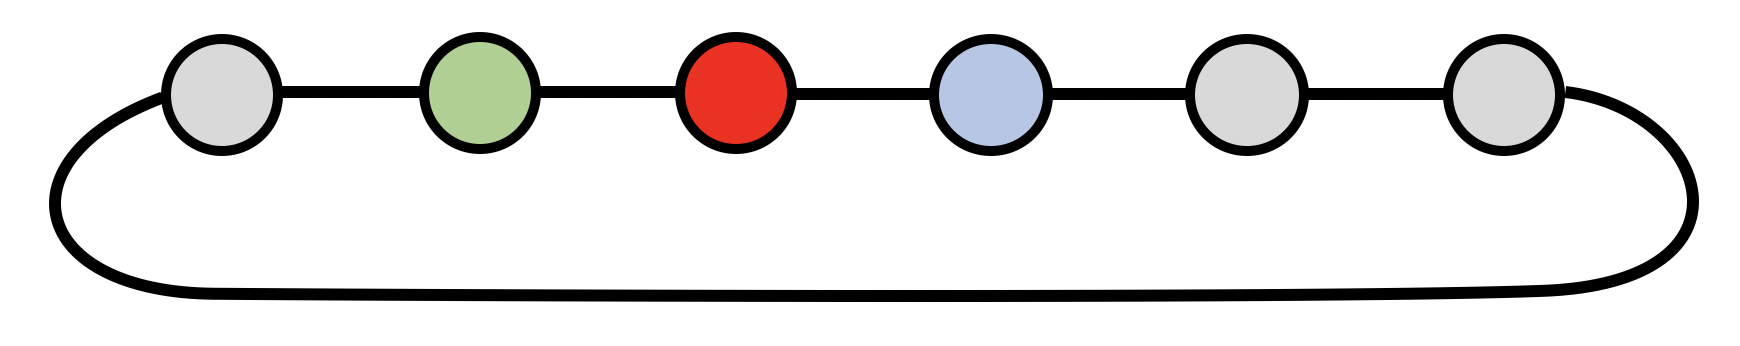
\includegraphics[width=0.9\linewidth]{figures/grid.png}
}，其节点编号为 $0, 1,\hdots, n-1$，并按 $n$ 取模（为简化记号，下文将省略模数），而且
邻接矩阵的元素满足 $a_{u,u+1 \, \mathrm{mod} \, n} = 1$，其余元素为零。它与此前讨论的一般图情形存在两个主要区别。
%
第一，每个节点 $u$ 都与其邻居 $u-1$ 和 $u+1$ 具有相同的连接方式，因而在结构上无法与其他节点区分。
%in terms of group theory, we say that the grid is a homogeneous space. 
\marginnote{正如后文将看到的，这使网格成为齐性空间。
  %  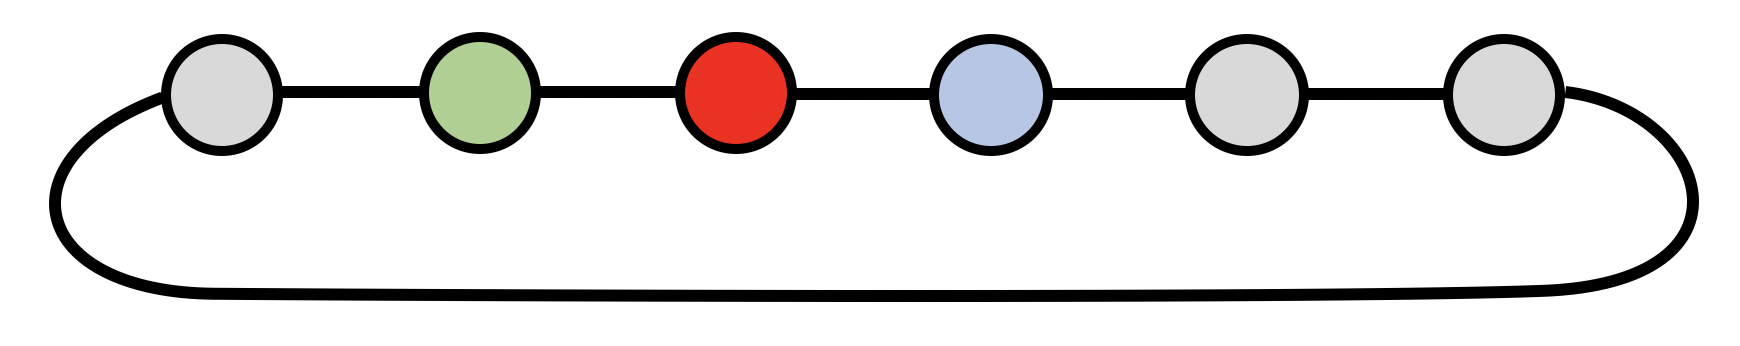
\includegraphics[width=1\linewidth]{figures/grid.png}
}
%
第二，也是更重要的一点，由于网格节点具有固定顺序，其{\em 邻居}也具有固定顺序：可以把 $u-1$ 称为“左邻居”，把 $u+1 $ 称为“右邻居”。
%
如果采用之前设计等变函数 $\mathbf{F}$ 的方案，并使用局部聚合函数 $\phi$，那么现在网格的每个节点上都有 $\mathbf{f}(\mathbf{x}_u) = \phi(\mathbf{x}_{u-1}, \mathbf{x}_{u}, \mathbf{x}_{u+1})$：$\phi$ 不再需要具有置换不变性。
%
%
对线性变换作特定选择 $\phi(\mathbf{x}_{u-1}, \mathbf{x}_{u}, \mathbf{x}_{u+1}) = \theta_{-1}\mathbf{x}_{u-1} + \theta_0 \mathbf{x}_{u} + \theta_1 \mathbf{x}_{u+1}$ 后，可以把 $\vec{F}(\mathbf{X})$ 写成矩阵乘积：
$$
\vec{F}(\mathbf{X}) = 
\left[
\begin{array}{ccccc}
\theta_0 & \theta_1  & & & \theta_{-1}\\
 \theta_{-1} & \theta_0 & \theta_1 & & \\
&  \ddots & \ddots & \ddots & \\
 &  & \theta_{-1} & \theta_0 & \theta_1\\
\theta_1 &  &  & \theta_{-1} & \theta_0

 \end{array}
  \right]
  %
\left[  
    \begin{array}{ccc}
    \horzbar & \mathbf{x}_0 & \horzbar \\
    \horzbar & \mathbf{x}_1 & \horzbar \\
             & \vdots    &          \\
    \horzbar & \mathbf{x}_{n-2} & \horzbar  \\           
    \horzbar & \mathbf{x}_{n-1} & \horzbar
  \end{array}
   \right]
$$
%
注意这种非常特殊的多对角结构：每条对角线上都重复同一个元素。在机器学习文献中，这有时称为“权重共享”。
%
%In machine learning literature, it is sometimes referred to as %``weight sharing'', a prominent feature of CNNs where the same %weights are applied at different positions in an image. 

%\michael{Notation: we denoted filters by $\theta$}

更一般地，给定向量 $\boldsymbol{\theta} = (\theta_0, \hdots, \theta_{n-1})$，{\em 循环矩阵}
$\mathbf{C}(\boldsymbol{\theta}) = (\theta_{u-v \, \mathrm{mod} \, n})$ 由向量 $\boldsymbol{\theta}$ 的循环移位版本依次排列得到。
%
循环矩阵与离散卷积等价，\marginnote{由于采用周期边界条件，这里是{\em 圆周卷积}或{\em 循环卷积}。在信号处理中，$\boldsymbol{\theta}$ 常称为“滤波器”；在 CNN 中，其系数是可学习的。}
%\taco{TODO: change this equation to a cross-correlation, and add a note saying that technically this is called a cc but we'll call it a conv.}
$$
(\mathbf{x} \star \boldsymbol{\theta})_u = \sum_{v=0}^{n-1}  x_{v \, \mathrm{mod}\, n} \,\, \theta_{u-v \, \mathrm{mod}\, n}
$$
%
因为有 $\mathbf{C}(\boldsymbol{\theta})\mathbf{x} = \mathbf{x} \star \boldsymbol{\theta}$。
%\petar{Should $i$ be replaced with $u$ in the equation above, given our blueprint? I did this in the CNN section.}
%
特定选择 $\boldsymbol{\theta}=(0,1,0,\hdots, 0)^\top$ 会产生一种特殊循环矩阵，它把向量向右移动一个位置。该矩阵称为（右）{\em 移位}或{\em 平移算子}，记为 $\mathbf{S}$。\marginnote{左移算子由 $\mathbf{S}^\top$ 给出。显然，先左移再右移（或反之）不会改变任何内容，这意味着 $\mathbf{S}$ 是{\em 正交的}：$\mathbf{S}^\top \mathbf{S} = \mathbf{S} \mathbf{S}^\top = \mathbf{I}$。}


%\michael{Notation: Replace $T$ by $S$}


%\michael{Naming: shift vs translation}


循环矩阵可以由其{\em 交换性}刻画：循环矩阵的乘积满足交换律，即
$\mathbf{C}(\boldsymbol{\theta}) \mathbf{C}(\boldsymbol{\eta}) = \mathbf{C}(\boldsymbol{\eta}) \mathbf{C}(\boldsymbol{\theta})$ 对任意 $\boldsymbol{\theta}$ 和 $\boldsymbol{\eta}$ 均成立。
%
由于移位是循环矩阵，便得到熟知的卷积算子{\em 平移等变性}或{\em 移位等变性}：
$$
\mathbf{S} \mathbf{C}(\boldsymbol{\theta}) \mathbf{x} = 
\mathbf{C}(\boldsymbol{\theta}) \mathbf{S} \mathbf{x}.
$$
%
这种交换性并不令人意外，因为底层对称群（平移群）是 Abel 群。
此外，反向结论似乎也成立，即
一个矩阵为循环矩阵，当且仅当它与移位算子可交换。
%
这又使我们能够把卷积{\em 定义}为平移等变的线性运算，并很好地展示了几何先验的力量以及几何 ML 的整体理念：卷积从平移对称性的第一性原理中自然产生。


注意，与集合和图上的情形不同，线性无关的移位等变函数（卷积）数量会随域的大小而\emph{增长}（因为循环矩阵的每条对角线都有一个自由度）。不过，尺度分离先验保证滤波器可以是{\em 局部的}，从而使每层仍具有相同的 $\Theta(1)$ 参数复杂度；在第~\ref{sec:cnnsec} 节讨论这些原则如何用于实现卷积神经网络架构时，我们将验证这一点。

%\joan{Link to GDL blueprint: 
%Convolutions also emerge as the essential device to build stable translation invariant representations, by querying the GDL blueprint. 
%Remark that, as opposed to the permutation group in sets and graphs, the number of linearly independent convolution maps \emph{grows} with the size of the domain (since we have one degree of freedom in each diagonal of a circulant matrix). However, the scale separation prior imposes only local filters, resulting in the same $\Theta(1)$-parameter complexity per layer, as we will verify in Section \ref{sec:cnnsec}.  }



\paragraph{离散 Fourier 变换的推导}
我们已经提到 Fourier 变换及其与卷积的联系：Fourier 变换能够对角化卷积运算，这一重要性质使信号处理中可以在频域通过 Fourier 变换的逐元素乘积执行卷积。
%
然而，教科书通常只陈述这一事实，很少解释 Fourier 变换究竟{\em 从何而来}，以及 Fourier 基为何如此{\em 特殊}。
%
这里将给出这一推导，再次说明对称性的基本原则何等根本。


为此，回顾线性\marginnote{还必须假设特征值互不相同，否则可能存在多个可能的对角化。我们所选的 $\mathbf{S}$ 满足这一假设。}代数中的一个事实：（可对角化）矩阵可以{\em 同时对角化}，当且仅当它们两两可交换。
%
换言之，所有循环矩阵都存在一个公共特征基，在该基下它们仅有特征值不同。
%
因此，可以任选一个循环矩阵并计算其特征向量——这些特征向量也必然是所有其他循环矩阵的特征向量。
%\taco{I think this is true only if all eigenvalues of this matrix are distinct. Take e.g. the identity matrix, which is circulant, and can be (re-)diagonalized by any orthogonal matrix. Using the shift operator is fine in this respect}\michael{The statement here is on the existence of a joint diagonalization. True, some circulant matrices have different bases diagonalizing them, but not all of them will diagonalize other matrices. }
选择移位算子最为方便，其特征向量恰好构成离散 Fourier 基。\marginnote{
$\mathbf{S}$ 正交但不对称，因此其特征向量相互正交，而特征值为复数（单位根）。
}
$$
\boldsymbol{\varphi}_k = \frac{1}{\sqrt{n}}\left (1, e^{ \frac{2\pi \mi k}{n}}, e^{ \frac{4\pi \mi k}{n} }, \hdots , e^{ \frac{2\pi \mi  (n-1)k}{n} }
\right)^\top, \hspace{5mm} k = 0, 1, \hdots, n-1,  
$$
%
可将这些向量排列为 $n\times n$ Fourier 矩阵 $\boldsymbol{\Phi} = (\boldsymbol{\varphi}_0, \hdots, \boldsymbol{\varphi}_{n-1})$。
% 
%
左乘 $\boldsymbol{\Phi}^*$\marginnote{注意，特征向量是复数，因此转置 $\boldsymbol{\Phi}$ 时需要取复共轭。}
得到离散 Fourier 变换（DFT），而左乘 $\boldsymbol{\Phi}$ 得到逆 DFT：
$$
\hat{x}_k = \frac{1}{\sqrt{n}}\sum_{u = 0}^{n-1}x_u e^{-\frac{2\pi \mi k u}{n} } \hspace{15mm}
%
{x}_u = \frac{1}{\sqrt{n}} \sum_{k = 0}^{n-1}\hat{x}_k e^{+\frac{2\pi \mi k u}{n} }.
$$

 
 
由于所有循环矩阵都可以同时对角化，\marginnote{
由于 Fourier 变换是正交矩阵（$\boldsymbol{\Phi}^* \boldsymbol{\Phi} = \mathbf{I}$），从几何上看，它相当于一次 $n$ 维旋转所对应的坐标系变换。在这一坐标系（“Fourier 域”）中，循环矩阵 $\mathbf{C}$ 的作用变为逐元素乘积。
}  
因而也都被 Fourier 变换对角化，
并且仅有特征值不同。由于循环矩阵 $\mathbf{C}(\boldsymbol{\theta})$ 的特征值就是滤波器的 Fourier 变换（例如见 \cite{bamieh2018discovering}），即 $\hat{\boldsymbol{\theta}} = \boldsymbol{\Phi}^* \boldsymbol{\theta}$，于是得到卷积定理：
$$
\mathbf{C}(\boldsymbol{\theta}) \mathbf{x} = \boldsymbol{\Phi}
\left[  
    \begin{array}{ccc}
    \hat{\theta}_0 &  &  \\
    & \ddots & \\
    & & \hat{\theta}_{n-1}
  \end{array}
   \right]\boldsymbol{\Phi}^*\mathbf{x}
   = \boldsymbol{\Phi} (\hat{\boldsymbol{\theta}} \odot \hat{\mathbf{x}} )
$$
%

由于 Fourier 矩阵 $\boldsymbol{\Phi}$ 具有特殊的代数结构，乘积 $\boldsymbol{\Phi}^\star \mathbf{x}$ 和 $\boldsymbol{\Phi} \mathbf{x}$ 可以利用快速 Fourier 变换（FFT）算法以 $\mathcal{O}(n \log n)$ 复杂度计算。这是频域滤波在信号处理中如此流行的原因之一；此外，滤波器通常直接在频域设计，因此从不显式计算其 Fourier 变换 $\hat{\boldsymbol{\theta}}$。


除了在教学上的价值之外，这里对 Fourier 变换
与卷积的推导还提供了一种把这些概念推广到图的方案。注意到环图的邻接矩阵恰好就是移位算子，便可以通过计算邻接矩阵的特征向量，构造图 Fourier 变换及卷积算子的类比（例如见 \cite{sandryhaila2013discrete}）。
%
早期通过类比 CNN 来发展图神经网络的尝试，有时称为“谱 GNN”，采用的正是这一蓝图。\marginnote{在图信号处理中，常用{\em 图 Laplacian} 的特征向量代替邻接矩阵来构造图 Fourier 变换，见 \cite{shuman2013emerging}。在网格上，这两个矩阵具有共同特征向量；但在图上，它们产生有所不同但彼此相关的构造。}
%
我们将在%Chapter~\ref{ch:graphs}
第~\ref{sec:manifolds}--\ref{sec:meshes} 节看到，
这一类比存在一些重要局限。
%
第一个局限源于网格是固定的，因此其上的所有信号都可以用同一个 Fourier 基表示。相比之下，在一般图上，Fourier 基依赖于图结构。因此，无法直接比较两个不同图上的 Fourier 变换——这一问题在机器学习任务中表现为缺乏泛化能力。
%
第二，多维网格由一维网格的张量积构造而成，并保留底层结构：Fourier 基元素及其对应频率（特征值）可以按多个维度组织。例如，在图像中，可以自然地讨论水平与垂直频率，滤波器也具有{\em 方向}概念。在图上，Fourier 域的结构是一维的，因为只能按对应频率的大小组织 Fourier 基函数。因此，图滤波器不感知方向，即具有{\em 各向同性}。



\paragraph{连续 Fourier 变换的推导}
为保证完整性，并为接下来的讨论作铺垫，我们在连续设定下重复上述分析。
与第~\ref{sec:scale_separation} 节类似，考虑定义在 $\Omega = \mathbb{R}$ 上的函数，以及平移算子 $(S_v f)(u) = f(u-v)$；该算子把 $f$ 平移某个位置 $v$。
 %
把 $S_v$ 施加到 Fourier 基函数 $\varphi_\xi(u) = e^{\mi \xi u}$ 上，利用指数运算的结合性得到
% \michael{Notation: same $\phi$ used to denote basis functions, filters, and local aggregators}
$$
S_v e^{\mi\xi u} = e^{\mi\xi (u-v)} = e^{-\mi\xi v} e^{\mi\xi u},
$$
即 $\varphi{u}_\xi(u)$ 是 $S_v$ 的复特征向量，对应复特征值 $e^{-\mi\xi v} $——这与离散设定下的情形完全一致。
由于 $S_v$ 是酉算子（即 $\| S_v x \|_p = \| x \|_p$ 对任意 $p$ 和 $x \in L_p(\R)$ 都成立），任意特征值 $\lambda$ 都必须满足 $|\lambda|=1$，这恰好对应于上面得到的特征值 $e^{-i\xi v}$。
此外，平移算子的谱是\emph{单谱}，即共享同一特征值的两个函数必然共线。事实上，假设 $S_v f = e^{-\mi \xi_0 v} f$ 对某个 $\xi_0$ 成立。对等式两边作 Fourier 变换，得到
$$\forall ~\xi~,~e^{-\mi \xi v} \hat{f}(\xi) = e^{-\mi \xi_0 v} \hat{f}(\xi)~,$$
这意味着 $\hat{f}(\xi)=0$ 对 $\xi \neq \xi_0$ 成立，因此 $f = \alpha \varphi_{\xi_0}$。

对于一般线性算子 $C$，若其具有平移等变性（$S_v C = C S_v$），则有
$$
S_v C e^{\mi\xi u} = C S_v e^{\mi\xi u} = e^{-\mi\xi v} C e^{\mi\xi u}, 
$$
这意味着 $C e^{\mi\xi u}$ 也是特征函数\marginnote{{\em 特征函数}与“特征向量”同义，用于指连续算子的特征向量。}，它属于 $S_v$，对应特征值 $e^{-\mi\xi v}$。
由谱的单谱性质可知 $C e^{\mi\xi u} = \beta \varphi_{\xi}(u)$；换言之，Fourier 基是所有平移等变算子的特征基。
%
因此，$C$ 在 Fourier 域中是\emph{对角的}，可以表示为 $C e^{\mi\xi u} = \hat{p}_{C}(\xi) e^{\mi\xi u}$，其中 $\hat{p}_{C}(\xi)$ 是作用于不同频率 $\xi$ 的{\em 传递函数}。
%
%
最后，对于任意函数 $x(u)$，由线性性可得
%\michael{Notation: use $\lambda$ in place of $\xi$ for frequency?}
%
\begin{eqnarray*}
(C x) (u) &=& C \int_{-\infty}^{+\infty} \hat{x}(\xi) e^{\mi \xi u} \mathrm{d}\xi = \int_{-\infty}^{+\infty} \hat{x}(\xi) \hat{p}_C(\xi) e^{\mi \xi u} \mathrm{d}\xi \\
&=& \int_{-\infty}^{+\infty} p_C(v) x(u-v) \mathrm{d}v~ = (x \star p_C)(u),\marginnote{The spectral characterisation of the translation group is a particular case of a more general result in Functional Analysis, the \emph{Stone's Theorem}, which derives an equivalent characterisation for any one-parameter unitary group.}
\end{eqnarray*}
%
其中 $p_C(u)$ 是 $\hat{p}_C(\xi)$ 的逆 Fourier 变换。因此，每个线性平移等变算子都是卷积。
% {\em quod erat demonstrandum}.










%\michael{Multi-dimensional grids = tensor products, multi-dimensional frequency space}


%
%Consider an Euclidean data domain $\Omega=[-A,A]^s$ with $s=1,2,3$, with $A$ either finite of infinite. 
%For $v \in \Omega$, a \emph{translation} $T_v: \Omega \to \Omega$ is defined as $T_v(u) = u - v$, where 
%the operation is periodized in the case of finite domain. 
%Local translation equivariant operators have a particularly concise representation, thanks to the 
%harmonic properties of Euclidean domains and the Abelian properties of the translation group. 
%Indeed, Abelian Groups are commutative. Linear operators $Q: L_2(\Omega) \to \L_2(\Omega)$ that 
%commute with translations can be completely characterized by first studying eigenfunctions 
%of the translation Group. 
%We verify that the Fourier atoms $g_\xi: u \mapsto \exp^{i \xi u}$ satisfy 
%$$T_v g_\xi (u) = g_\xi(u-v) = \exp^{i \xi (u-v)} = \exp^{-i v \xi} g_\xi(u)~$$
%and therefore that $g_\xi$ is a (complex) eigenvector of the translation group, with (complex) eigenvalue $\exp^{-i v \xi}$. 
%Consider now $Q$ that commutes with any translation. We have 
%$$T_v Q g_\xi = Q T_v g_\xi = \exp^{-i v \xi} Q g_\xi~,$$
%which means that $Q g_\xi$ is also an eigenvector of $T_v$ with eivenvalue $\exp^{-i v \xi}$. Thus $Q g_\xi = c_{Q}(\xi) g_\xi$, 
%or, in other words, $Q$ is \emph{diagonal} in the Fourier domain. By linearity, we obtain 
%$$Q x (u) = Q \int \hat{x}(\xi) g_\xi d\xi = \int \hat{x}(\xi) c_{Q}(\xi) g_\xi = \int h_Q(v) x(u-v) dv~,$$
%where $h_Q$ is the inverse Fourier transform of $c_Q$. 
%Convolutions are thus the only linear translation equivariant operators. 
%
%A discrete grid is obtained by discretizing or \emph{sampling} $\Omega$ at a certain rate $N$, resulting in $\Omega_d = \{ \frac{1}{N}(i_1, \dots i_s); i_j \in [-AN,AN] \}$. We verify that the same analysis can be carried out in this discrete domain, by replacing the continuous Fourier transform by its discrete analog. . 
%



% Consider basing this on Michael's blog post https://towardsdatascience.com/deriving-convolution-from-first-principles-4ff124888028
% That is, derive convolution as the most general linear translation-equivariant map

\subsection{群与齐性空间}
\label{sec:groups}

%\joan{ Joan: the blueprint is described in general for groups, so perhaps the emphasis of this section should be  to describe canonical instances of the blueprint on non-commutative Lie groups, or domains that exhibit a geometric property not found in the previous sections. 
%In that sense, each subsection introduces a different key aspect. Sets: permutation symmetry with `trivial' group representation, no metric; Graphs: less trivial representation (conjugation) with metric. 
%Grids: commutative group action, homogeneous space. 
%Lie Groups: non-commutative, homogeneous space. 
%Gauges: ??
%}

%\michael{Michael: I actually thought that here we would like to still treat the plane, but generalize translations to more complex transformations, introducing the generalization of Fourier through representation theory (which is parallel to the generalization we do through spectral analysis). I don't think it makes sense to repeat permutations here once more. The next section will describe non-homogeneous spaces (manifolds)
%}

%\taco{Taco: decision from meeting: this section will focus on continuous examples, e.g. spherical CNNs.} 

% Introduce regular representation & induced representation. 
% Most general linear map is again a (generalized) convolution


%\michael{
%Rectify notation to be consistent. Get rid of references to CNNs - this comes in the later section. 
% Decide if we use `shift' or `translation'} % TC: Let's use shifts


关于网格的讨论突出了移位与卷积之间的紧密联系：卷积是线性移位等变运算。\marginnote{严格来说，需要群是{\em 局部紧致的}，从而存在左不变 Haar 测度。关于该测度积分时，可以用任意群元素“移位”被积函数而得到相同结果，正如
$$
\int_{-\infty}^{+\infty} \hspace{-2mm} x(u) \mathrm{d}u = \int_{-\infty}^{+\infty} \hspace{-2mm} x(u - v) \mathrm{d}u
$$ 
对函数 $x : \R \rightarrow \R$ 成立。}反过来，任意移位等变线性算子都是卷积。
%
此外，移位算子可以由 Fourier 变换同时对角化。
%
事实证明，这只是一个更宏大理论的一部分：只要能够在某个对称群上求和或积分，就可以{\em 为任意这样的对称群}定义卷积与 Fourier 变换。



考虑 Euclidean 域 $\Omega = \mathbb{R}$。
可以把卷积理解为模式匹配运算：将滤波器 $\theta(u)$ 的移位副本与输入信号 $x(u)$ 匹配。
卷积 $(x \star \theta)(u)$ 在点 $u$ 处的值，是信号 $x$ 与\emph{平移了 $u$ 的}滤波器之间的内积：
$$
(x \star \theta)(u) =  \langle x, S_u \theta \rangle  = \int_\R x(v)\theta(u + v)  \mathrm{d}v.\marginnote{Note that what we define here is not convolution but {\em cross-correlation}, which is tacitly used in deep learning under the name `convolution'. We do it for consistency with the following discussion, since in our notation $(\rho(\fg)x)(u) = x(u-v)$ and $(\rho(\fg^{-1})x)(u) = x(u+v)$.}
$$
%
注意，在这种情形下，$u$ 既是{\em 域 $\Omega = \R$ 上的点}，也是{\em 平移群的元素}；该平移群可以与域本身等同，即 $\fG = \R$。
下面说明如何推广这一构造：只需把平移群替换为另一个群 $\fG$，并让它作用在 $\Omega$ 上。
%The basic idea of \emph{group convolution} is to match $f$ with transformed copies of $\theta$, where now the transformations are taken from $\fG$.

\paragraph{群卷积}
%Following the Geometric Deep Learning blueprint, we start with a group $\fG$ acting on a domain $\Omega$. 
正如第~\ref{sec:geom_priors} 节所讨论的，群 $\fG$ 在域 $\Omega$ 上的作用
诱导出表示 $\rho$，即 $\fG$ 在信号空间 $\mathcal{X}(\Omega)$ 上的表示，
%of signals on $\Omega$, 
其作用方式为 $\rho(\fg) x(u) = x(\fg^{-1} u)$。
在上述例子中，$\fG$ 是平移群，其元素通过 $u+v$ 平移坐标；而 $\rho(\fg)$ 是作用于信号的移位算子，满足 $(S_v x)(u) = x(u-v)$。
最后，为了把滤波器应用于信号，我们调用 $\mathcal{X}(\Omega)$ 是 Hilbert 空间这一假设，并使用内积
\begin{equation*}
    \langle x, \theta \rangle = \int_{\Omega} x(u) \theta(u) \mathrm{d}u, \marginnote{The integration is done w.r.t. an invariant measure $\mu$ on $\Omega$. In case $\mu$ is discrete, this means summing over $\Omega$. } %\mu(u),
\end{equation*}
其中为简单起见假设信号为标量值信号 $\mathcal{X}(\Omega,\mathbb{R})$；一般情况下，内积具有式~（\ref{eqn:innerprod}）的形式。
%, see Section~\ref{sec:geom_priors}. 

% As per the GDL blueprint (Section \ref{}), we need to choose a 
% %In order to make this idea precise, 
% %we need to define three things: the 
% space of signals $\mathcal{X}(\Omega)$, a group $\fG$ acting on it, and an inner product $\langle \cdot, \cdot \rangle$ between these signals.
% %For example, for the choices of $\Omega=\mathbb{Z}_n$ (one-dimensional grid), $\mathbb{R}^2$ (plane), or $\mathbb{S}^2$ (sphere), $\fG$ is the respective symmetry group of that domain (cyclic shifts, roto-translations, and 3D rotations). 
% %
% %
% As shown in Section~\ref{sec:symmetries}, 
% from the action of $\fG$ on the domain $\Omega$, we can derive the action of $\fG$ on the signals  $\mathcal{X}(\Omega)$ through the representation
% %\taco{Consider moving this to an earlier section.}\michael{Agree, move to 1.2.1. and just mention here}
% $
% 	\rho(\fg) x(u) = x(\fg^{-1} u)
% $
% %using to the notation we adopted  
% In the above example, $\fG$ is the translation group whose elements act by shifting the coordinates, $u+v$, whereas $\rho(\fg)$ is the shift operator acting on signals as $(T_v x)(u) = x(u-v)$. 
% %\taco{Consider designating one symbol, e.g. $T$ or $\rho$ for the regular representation, and using that throughout.}\michael{Lets use $\rho$. here $T$ is a specific example}
% %
% %Similarly, when $\fG$ is the roto-translation group, the operator $\rho(\fg)$ tells us how to rotate and translate a signal. 
% %
% Finally, in order to apply a filter to the signal, we invoke our assumption of $\mathcal{X}(\Omega)$ being a Hilbert space, with an inner product 
% %
% %we need to specify an inner product, which typically takes the form \taco{TODO:consider moving this to the definition of $\mathcal{X}(\Omega)$, i.e. define it as a Hilbert space?}
% \begin{equation*}
%     \langle x, \theta \rangle = \int_{\Omega} x(u) \theta(u) du. \marginnote{The integration is done w.r.t. an invariant measure $\mu$ on $\Omega$. In case $\mu$ is discrete, this means summing over $\Omega$. } %\mu(u),
% \end{equation*}
% (where we assumed, for the sake of simplicity, scalar-valued signals, $\mathcal{X}(\Omega,\mathbb{R})$; in a more general case, the inner product has the form of equation~(\ref{eqn:innerprod}), see Section~\ref{sec:geom_priors}). 
% %where $\mu$ is an invariant measure on $\Omega$ \michael{Perhaps write it simply as $du$, and put a margin note?}. % too technical?
% %In the case where $\mu$ is discrete, the inner product is a sum over the ``dimensions'' $x$ of the product of the vector components $f(x) \theta(x)$. 
% %



如此定义了信号的变换方式以及信号与滤波器的匹配方式后，便可以为 $\Omega$ 上的信号定义{\em 群卷积}：
\begin{equation}
    \label{eq:group-conv}
    (x \star \theta)(\fg) = \langle x, \rho(\fg) \theta \rangle = \int_\Omega x(u) \theta(\fg^{-1} u) \mathrm{d}u. %\mu(x).
\end{equation}
%
注意，$x \star \theta$ 的取值对象是{\em 元素} $\fg$，即{\em 群} $\fG$ 的元素，而不是域 $\Omega$ 上的点。
因此，下一层以 $x \star \theta$ 为输入时，应当
作用于定义%on the domain
{\em 在群} $\fG$ {\em 上的}信号，%use the domain $\Omega' = \fG$;
稍后将回到这一点。

正如传统 Euclidean 卷积具有移位等变性，
更一般的群卷积具有 $\fG$-{\em 等变性}。
关键观察是：将信号 $x$ 与经过 $\fg$ 变换的滤波器 $\rho(\fg) \theta$ 匹配，等价于将经过逆变换的信号 $\rho(\fg^{-1}) x$ 与未变换的滤波器 $\theta$ 匹配。
%Operators satisfying these relation are called {\em adjoint}, denoted by 
%$\rho(\fg)^* = \rho(\fg^{-1})$ and can be exchanged under the inner product, 
%$$
%\langle x, \rho(\fg) \theta \rangle = \langle \rho(\fg^{-1}) x, \theta \rangle\marginnote{This implies that $\rho$ is \emph{unitary} with respect to the inner product $\langle, \rangle$, and can be derived from the definition of the inner product and the invariant integral, see e.g. [CITE Folland, Spherical CNNs].}
%$$
数学上可表示为 $\langle x, \rho(\fg) \theta \rangle = \langle \rho(\fg^{-1}) x, \theta \rangle$。
%
%$\rho(\fg)$ is adjoint to $\rho(\fg^{-1})$ which means that $\langle x, \rho(\fg) \theta \rangle = \langle \rho(\fg^{-1}) x, \theta \rangle$\marginnote{This implies that $\rho$ is \emph{unitary} with respect to the inner product $\langle, \rangle$, and can be derived from the definition of the inner product and the invariant integral, see e.g. [CITE Folland, Spherical CNNs]}.
%
有了这一观察，$\fG$-等变性对于群卷积~（\ref{eq:group-conv}）便由其定义以及群表示的定义性质 $\rho(\fh^{-1}) \rho(\fg) = \rho(\fh^{-1} \fg)$ 直接得到：
%is easy:
% \begin{equation}
%     \begin{aligned}
%         ((\rho(\fh) x) \star \theta)(\fg)
%         &= \langle \rho(\fh) x, \rho(\fg) \theta \rangle \\
%         &= \langle x, \rho(\fh^{-1}) \rho(\fg) \theta \rangle \\
%         &= \langle x, \rho(\fh^{-1} \fg) \theta \rangle \\
%         &= (x \star \theta)(\fh^{-1} \fg) \\
%         &= (\rho(\fh) (x \star \theta))(\fg)
%     \end{aligned}
% \end{equation}
\begin{equation*}
    (\rho(\fh) x \star \theta)(\fg)
    = \langle \rho(\fh) x, \rho(\fg) \theta \rangle
    %= \langle x, \rho(\fh^{-1}) \rho(\fg) \theta \rangle
    = \langle x, \rho(\fh^{-1} \fg) \theta \rangle
    %= (x \star \theta)(\fh^{-1} \fg)
    = \rho(\fh) (x \star \theta)(\fg).
\end{equation*}
%In the first step, we use the definition of group convolution.
%In the second, we use adjointness together with the property of the representation %$\rho(\fh^{-1}) \rho(\fg) = \rho(\fh^{-1} \fg)$. % (because $\rho$ is a representation).
%In the last step we again use the definition of convolution, as well as the definition of $\rho$. 

% \michael{Comment on commutativity}


下面来看几个例子。
上文研究的一维网格情形对应如下选择：
$\Omega = \Z_n = \{0, \ldots, n-1\}$，循环移位群为 $\fG = \Z_n$。
%
在这种情形下，群元素是索引的循环移位，即元素 $\fg \in \fG$ 可以与某个 $u = 0,\hdots, n-1$ 等同，使得 $\fg. v = v - u \, \mathrm{mod} \, n$；其逆元素为 $\fg^{-1}. v = v + u \, \mathrm{mod} \, n$。重要的是，在本例中，{\em 群}的元素（移位）也是{\em 域}的元素（索引）。
%
%The representation is the shift operator $\rho(\fg) = \mathbf{S}^i$. 
%
%With some abuse of notation, we can therefore write 
因此，稍微滥用记号，可以把这两个结构等同起来（即 $\Omega = \fG$）；此时群卷积的表达式
$$
%(x \star \psi)(\fg) =  \sum_{j=0}^{n-1} x_j \, \psi_{j - \fg \,\, \mathrm{mod} \, n},
(x \star \theta)(\fg) =  \sum_{v=0}^{n-1} x_v \, \theta_{\fg^{-1} v},
%\marginnote{Note that the reflection of the filter in the standard convolution stems from the user of $\fg^{-1}$ rather than $\fg$. } Taco: this is not true; this equation is actually a cross-correlation which does not involve flipping the filter. In a convolution, one of the appearances of u (ie j) is inverted. 
$$
导出熟悉的卷积\marginnote{严格来说，这里同样是互相关。}$\displaystyle (x\star \theta)_u = \sum_{v=0}^{n-1} x_v \, \theta_{v + u\,\, \mathrm{mod} \, n}$。



\paragraph{球面卷积}
现在考虑
\marginnote{
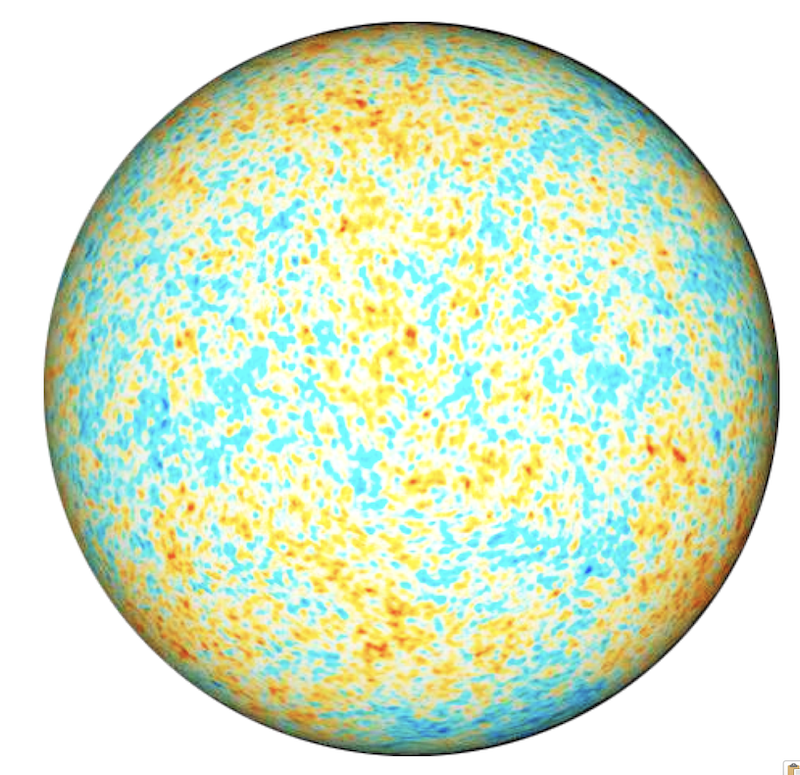
\includegraphics[width=0.9\linewidth]{figures/planck.png}
Planck 空间天文台观测到的宇宙微波背景辐射是 $\mathbb{S}^2$ 上的信号。
}
二维球面 $\Omega = \mathbb{S}^2$，其旋转群为{\em 特殊正交群} $\fG = \mathrm{SO}(3)$。
%
尽管选择该例是出于教学目的，但它实际上非常实用，并出现在大量应用中。例如，在天体物理学中，观测数据往往天然具有球面几何。此外，在化学应用中对分子建模并预测其性质时，球面对称性也十分重要，例如可用于虚拟药物筛选。
%\michael{ADD: molecules/astrophysics}


把球面上的点表示为三维单位向量 $\mathbf{u} : \|\mathbf{u}\|=1$ 后，群作用可以表示为 $3\times 3$ 正交矩阵 $\mathbf{R}$，并满足 $\mathrm{det}(\mathbf{R}) = 1$。因此，球面卷积可以写成信号与旋转后滤波器的内积：
$$
(x\star \theta)(\mathbf{R}) = \int_{\mathbb{S}^2} x(\textbf{u}) \theta(\mathbf{R}^{-1}\mathbf{u}) \mathrm{d}\mathbf{u}.
\marginnote{
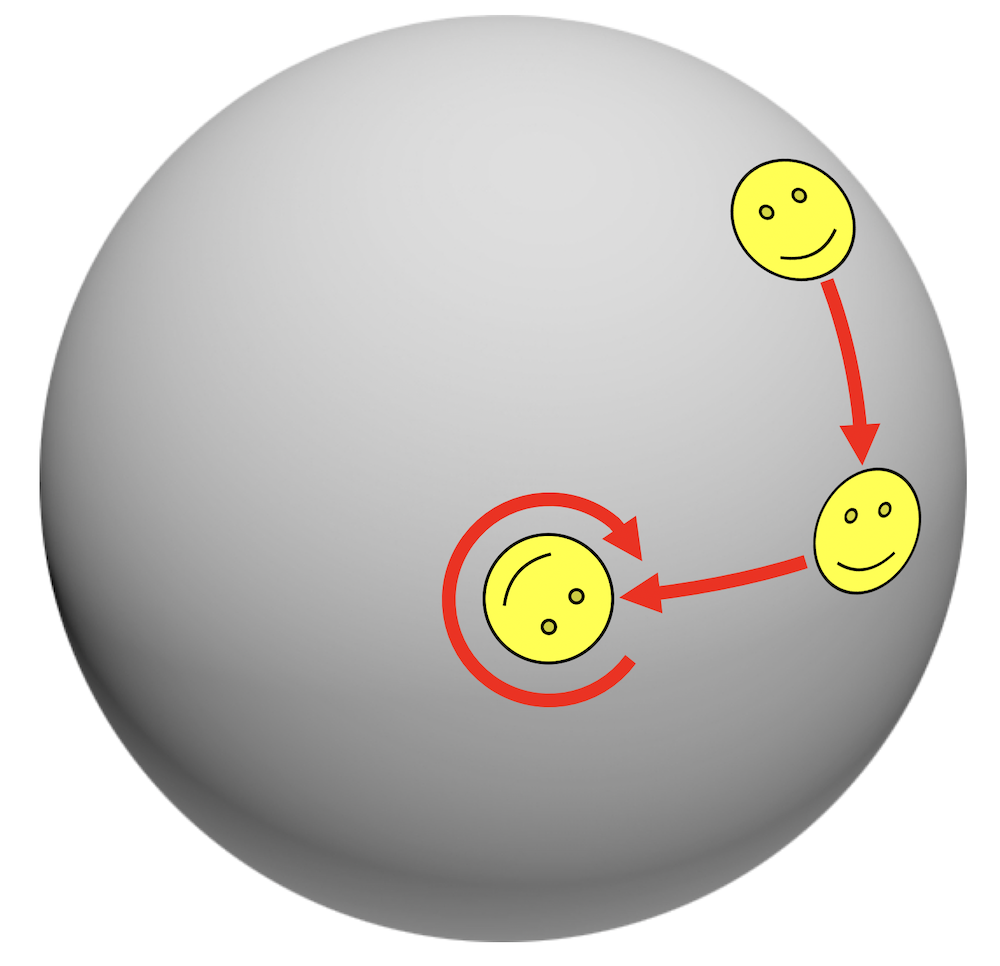
\includegraphics[width=0.9\linewidth]{figures/so3.png}
The action of $\mathrm{SO}(3)$ group on $\mathbb{S}^2$. Note that three types of rotation are possible; the $\mathrm{SO}(3)$ is a three-dimensional manifold.  
}
$$


首先应注意，此时群与域并不相同：群 $\mathrm{SO}(3)$ 是 Lie 群，事实上是三维流形；而 $\mathbb{S}^2$ 是二维流形。
%
因此，与前一个例子不同，这里的卷积是定义{\em 在} $\SO{3}$ {\em 而非} $\Omega$ {\em 上的}函数。

%\michael{\bf [ADD: a figure showing the difference between the sphere and SO(3) and why integration on S would give only isotropic filters.]}


这会带来重要的实际后果：在几何深度学习蓝图中，我们把后续算子应用于前一个算子的输出，以此串接多个等变映射（在深度学习术语中称为“层”）。
%
在平移情形下，可以依次应用多个卷积，因为它们的输出都定义在同一个域 $\Omega$ 上。
%
在一般设定下，由于 $x \star \theta$ 是定义在 $\fG$ 而非 $\Omega$ 上的函数，后续不能使用完全相同的运算——这意味着下一个运算必须处理{\em $\fG$ 上的信号}，即 $x \in \mathcal{X}(\fG)$。
%
群卷积的定义允许处理这种情形：
把域取为 $\Omega = \fG$，并让 $\fG$ 自身通过群作用 $(\fg, \fh) \mapsto \fg \fh$ 作用于它；该作用由 $\fG$ 的复合运算定义。
由此得到表示 $\rho(\fg)$，它作用于 $x \in \mathcal{X}(\fG)$，其作用方式为 $(\rho(\fg) x)(\fh) = x(\fg^{-1}\fh)$。\marginnote{$\fG$ 作用于定义在 $\fG$ 自身上的函数时，其表示称为 $\fG$ 的\emph{正则表示}。}
% where $\fg, \fh$ and their composition $\fg^{-1}\fh$ belong to the group $\fG$.
与之前一样，内积通过在域上积分%product of $x$ and $\psi$
信号与滤波器的逐点乘积来定义；
此时该域为 $\Omega = \fG$。
%
因此，在球面卷积的例子中，第二个卷积层具有如下形式：
$$
((x\star \theta)\star \phi)(\mathbf{R}) = \int_{\mathrm{SO}(3)} (x\star \theta)(\textbf{Q}) \phi(\mathbf{R}^{-1}\mathbf{Q}) \mathrm{d}\mathbf{Q}.
$$


%Now consider $\Omega = \R^2$ with  the group $\fG = \SE{2}$ of planar rotations and translations.\marginnote{$\SE{2}$ is called the {\em special Euclidean group} and is a subgroup of the Euclidean (isometry) group that additionally includes reflection. } 
%The first thing to note is that now the group elements (roto-translations) are not identical to the points on the domain. Consequently, in this case, unlike the previous example, the group convolution $x\star \psi$ given as the inner product between the signal and the transformed filter is a function {\em on} $\SE{2}$ {\em rather than on} $\Omega$. 

%\taco{TODO: Figure of SE2 group conv. Both planar to group, and group to group.}




%Our construction can be generalized to signals on any (locally compact) group $\fG$ and any $\Omega$ acted on by $\fG$ (in a sufficiently nice way).
%$\Omega$ is said to be a {\em homogeneous space} if for any two points $u, v \in \Omega$ one can be transformed into another, $u = \fg v$, by a symmetry $\fg \in \fG$. 
%that maps one to the other, .
%As noted before, for any such space $\Omega$, we have a regular representation $\rho(\fG)$ of $\fG$ acting on the space of signals $\mathcal{X}(\Omega)$. \michael{Bring the definition of homogeneous space earlier to Sec 1.2.1}
%
%As we will show in Chapter ???, for any two homogeneous spaces $\Omega$ and $\Omega'$ and a group $\fG$, one can define a convolution that maps between $\mathcal{X}(\Omega)$ and $\mathcal{X}(\Omega')$ in an equivariant manner, and indeed the most general linear equivariant map between these spaces is a convolution.

由于卷积涉及内积，而内积又需要在域 $\Omega$ 上积分，所以只能在规模较小（离散情形）或维数较低（连续情形）的域 $\Omega$ 上使用卷积。
% 
例如，可以在平面 $\R^2$（二维）、特殊正交群 $\SE{3}$（三维）或图的有限节点集合（$n$ 维）上使用卷积；但在实践中无法在置换群 $\Sigma_n$ 上执行卷积，因为该群含有 $n!$ 个元素。
%
同样，在更高维的群（如仿射群，其中包含平移、旋转、剪切和缩放，共有 $6$ 个维度）上积分，在实践中并不可行。
%
尽管如此，正如第~\ref{sec:gnn-intro} 节所见，通过处理定义在低维空间上的信号，仍可以为大群 $\fG$ 构造等变卷积；这里的低维空间为 $\Omega$，且 $\fG$ 作用于其上。
事实上，可以证明，两个域之间的任意等变线性映射 $f : \mathcal{X}(\Omega) \rightarrow \mathcal{X}(\Omega')$，其中两个域为 $\Omega, \Omega'$，都可以写成类似于这里所讨论群卷积的广义卷积。%\michael{Taco: I don't understand what you want to say here.}

其次，注意到上一节从卷积的移位等变性质推导出的 Fourier 变换，也可以通过把信号投影到对称群不可约表示的矩阵元素上，推广到更一般的情形。后续工作将对此展开讨论。
%
对于这里研究的 $\SO{3}$，这会产生{\em 球谐函数}与 {\em Wigner D-functions}，它们在量子力学和化学中有广泛应用。


最后指出支撑本节此前讨论的一项假设：无论 $\Omega$ 是网格、平面还是球面，我们都可以把任意一点变换为任意另一点；直观而言，这意味着域上的所有点“看起来都一样”。% by means of a rotation
%
具有这一性质的域 $\Omega$ 称为{\em 齐性空间}；对任意 $u, v\in \Omega$，都存在 $\mathfrak{g}\in\fG$ 使得
$
\mathfrak{g}.u = v\marginnote{The additional properties, $\mathfrak{e}.u = u$ and $\mathfrak{g} (\mathfrak{h}. u) = (\mathfrak{gh}). u$ are tacitly assumed here. }
$.
%
下一节将尝试放宽这一假设。

%Consider as given a space $\Omega$, such as $\Omega = \R^2$, $\Omega = \Z^2$, or $\Omega = S^2$ (the sphere).
%Furthermore, let $G$ be a group of symmetries acting on $\Omega$, such as the group of roto-translations acting on $\R^2$, or the group or 3D rotations acting on the sphere.
%The inputs and feature maps of our generalized CNN are modelled as signals on $\Omega$, defined as $\mathcal{X}_\Omega = \{f : \Omega \rightarrow \R\}$\marginnote{In practice one would usually want to use multiple channels $c$, i.e. $f : \Omega \rightarrow \R^c$ but to reduce clutter we consider a single channel / grayscale image for now.}.
%From the action of $G$ on $\Omega$, we can derive an action of $G$ on $\mathcal{X}_\Omega$:
%\begin{equation}
%	\rho(g) f(x) = f(g^{-1} x)
%\end{equation}
%When $G$ is the translation group, this is just the \emph{shift operator} defined in the previous section.
%Similarly, when $G$ is the roto-translation group, this operator tells us how to roto-translate an image of filter $f$.

%In order to match a filter and an image / feature map, we define an inner product:
%\begin{equation}
%    \langle f, \psi \rangle = \int_{\Omega} f(x) \psi(x) d\mu(x),
%\end{equation}
%where $\mu$ is an invariant measure on $\Omega$. % too technical?
%In the case where $\mu$ is discrete, the inner product is a sum over the ``dimensions'' $x$ of the product of the vector components $f(x) \psi(x)$. 

%Having defined how to transform filters and match patterns, we are ready to define the generalized convolution:
%\begin{equation}
%    \label{eq:group-conv}
%    f \star \psi(g) = \langle f, \rho(g) \psi \rangle = \int_\Omega f(x) \psi(g^{-1} x) %d\mu(x).
%\end{equation}

%Let's look at some examples.
%When $\Omega = \Z_n = \{1, \ldots, n\}$ and $G = \Z_n$ (i.e. we consider signals on $\Z_n$ and the group of cyclic shifts) as in the last section, we retrieve the usual discrete convolution.
%To see this, note that $g^{-1} x$ in the equation above means: invert the group element $g \in G$ (in this example, the inverse of $g \in \Z_n$ is $-g$) and then act on $x \in \Omega$ (in this example, we get $x - g$.
%So the equation boils down to $f \star \psi(g) = \sum_i f(i) f(i - g)$.

%Now consider $\Omega = \R^2$ and $G = \SE{2}$, the group of rotations and translations acting on the plane.
%The first thing to note is that $f \star \psi$ is a function on $G = \SE{2}$ rather than a function on $\Omega$.
%In the previous example $\Omega = G$ so the distinction does not matter, but here it does.
%The group convolution computes the similarity between the input and filter for each transformation of the filter.



%Since the feature map $f \star \psi$ is a function on $G$ rather than $\Omega$, we cannot use exactly the same operation for the second and higher layers of the network.
%The solution is easy enough, though: for the second layer we define $\Omega_2 = G$, so that the feature space consists of functions $f : G \rightarrow \R$.
%We again define a shift operator $\rho_2(g)$ acting on such functions by $(\rho(g) f)(h) = f(g^{-1} h)$, where now $g^{-1} h$ refers to composition in the group $G$ (c.f. $g^{-1} x$ for $x \in \Omega$ refering to the group action of $G$ on $\Omega$).
%With these definitions, the exact same Equation \ref{eq:group-conv} defines the group convolution for second and higher layers.

%As a final example, consider spherical CNNs.
%Here we take the domain $\Omega_1 = S^2$ (the sphere) for the input space, and $G = \SO{3}$ the rotation group as symmetries.

%\taco{TODO: all of the above should be more conversational. Maybe focus on one example?}

%\michael{Generalised Fourier transform using representation theory. Bring up again the notion of multidimensional frequencies and show here where it comes from. }


%\michael{{\bf Say something along the lines:} 
%The important difference between the above examples and the case of sets and graphs is that on the grid, plane, or sphere we can represent our group with a small number of parameters: in case case of $\Z_n$, this is just one index, in the case of $\mathbb{R}^2$, this is translation vector and rotation angle, and in the case of the sphere ... 
%
%Conversely, on sets or graphs, the permutation group does not have such a low-dimensional representation and has a combinatorial complexity. 

%Show again why on graphs we don't have multi-dimensional Fourier transform. 
%}

%\michael{Talk about homogeneous vs non-homogenous spaces, using the example of graphs. Make it a segway to the next section}


%[Fourier theory]


\subsection{测地线与流形}
\label{sec:geomanifoldsec}
%\michael{\bf [TACO: pls check if you are ok with this narrative. I start with homogeneous spaces, manifolds, then parallel transport. Then we can say that there is a broader view and talk about bundles in general]}

%\joan{
%Some high-level comments on what's written so far. 
%The generalization from groups to gauges is non-trivial, and I think it would be helpful to illustrate this extra level of generality with a running example. 
%In particular, an important innovation is that now we associate input data to certain vector fields on the domain; this is different from before. 
%It seems that this is the setting where the gauge equivariance is best motivated (unless I missed something), and I assume we can still use certain tasks from particle physics to motivate it.
%In other words, so far in our previous applications, the symmetry group acts on signals $\mathcal{X}(\Omega, \gV)$ only through $\Omega$, leaving the channels unchanged (just transporting them along the group action in $\Omega$). Now the situation is different and the gauge transformation is acting on the channels. 
%}

%\joan{I had a quick pass and the section reads very well; the build-up is coherent and objects are introduced keeping the intuition in mind (and adding figures to the margins will be even more helpful. 

%In particular, we can highlight that, contrary to the previous example of a fixed (curved) domain, many applications consider a variable geometric domain, and we wish to obtain signal representations that satisfy certain properties, namely (i) they are intrinsic, ie since the domain is defined only up to isometry, the signal representation should be invariant to isometries, and (ii) stability properties as this geometric domain changes. 
%These two aspects require introducing minimal elements of riemannian geometry 

%I have one comment/question though: currently we introduce the "minimal" elements of riemanian geometry that allow us to define convolutions and to describe the natural symmetries arising in manifold data (in particular isometry). 
%Would it be possible/convenient to highlight the invariance/stability priors early on, to motivate even further the need to introduce the different concepts (connection, parallel transport, isometries, geodesics, etc). In other words, the starting point is that we want to estimate a function $f$ defined over $\gX(\Omega, \R^s)$ that satisfies certain priors. The first and most natural prior is that $f$ is defined up to isometric transformations of $\Omega$. The second (if appropriate) is again the scale separation, ie local statistics in $x \in \gX(\Omega, \R^s)$ dominate. Then we explain how these priors lead again naturally to the GDL template by appropriately extending the notion of convolution. Additionally, it could be pertinent to describe how these priors relate to the stability of $f$ with respect to small changes in the metric structure of $\Omega$. 


%}


在上一个例子中，%domain $\Omega$ was the
球面 $\mathbb{S}^2$ \marginnote{旋转群 $\mathrm{SO}(3)$ 也是如此，因为它是{\em Lie 群}。}
是一个{\em 流形}，尽管它是一种特殊流形，
%: every point $u$ on $\mathbb{S}^2$ can be rotated into any other point $v$, intuitively meaning that all the points on the sphere ``look the same.'' % by means of a rotation  
%
%A domain $\Omega$ with such property is called a {\em homogeneous space}, where for any $u, v\in \Omega$ there exists %$\frak{g}\in\fG$ such that 
%$
%\frak{g}.u = v\marginnote{The additional properties, %$\frak{e}.u = u$ and $\frak{g}.(\frak{h}.u) = (\frak{gh}).u$ %are tacitly assumed here. }
%$.
%%
%Homogeneous spaces thus have a 
其齐性结构使它具有全局对称群。
%
遗憾的是，大多数流形并非如此，它们通常不具有全局对称性。
%
在这种情形下，无法直接定义 $\fG$ 在 $\Omega$ 上信号空间中的作用，也无法利用它使滤波器四处“滑动”，从而把卷积定义为经典构造的直接推广。
%. \joan{why would we want to translate signals in the manifold?}
%
尽管如此，流形确实具有两类不变性%symmetries
%various kinds of \emph{local} symmetries 
，本节将对此加以探讨：保持度量结构的变换，以及局部参考标架的变化。
%local \emph{gauge symmetries}, which we will now explore. 

尽管对许多机器学习读者而言，流形可能显得有些陌生，但它们在各种科学领域中其实非常常见。在物理学中，流形作为宇宙模型发挥核心作用——根据 Einstein 的广义相对论，引力源于时空的曲率，而时空被建模为伪 Riemann 流形。
%
在计算机图形学与视觉等较为“日常”的领域，流形是三维形状的常用数学模型。\marginnote{“3D”一词略有误导性，它指的是{\em 嵌入空间}。形状本身是二维流形（曲面）。}%
%
这类模型的应用范围十分广泛，从虚拟现实、增强现实以及通过“动作捕捉”获得的
特效，到研究蛋白质相互作用的结构生物学；蛋白质会像三维拼图块一样黏合在一起（化学术语称为“结合”）。
%
这些应用的共同之处，是使用流形表示某个三维对象的边界曲面。


这类模型之所以便利，有以下几个原因。\marginnote{
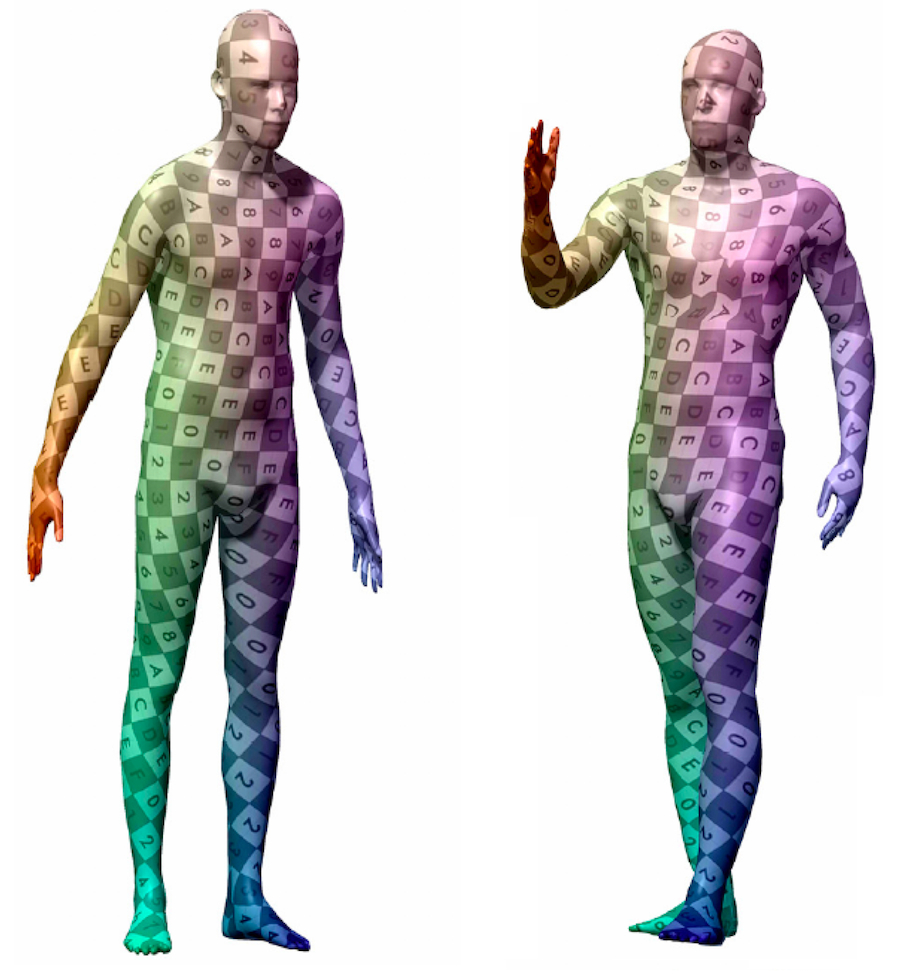
\includegraphics[width=0.9\linewidth]{figures/humans.png}
人体是以近似等距方式发生形变的非刚性对象实例。
}第一，它们可以紧凑地描述三维对象，无需像基于网格的表示那样为“空白空间”分配内存。
%
第二，它们允许忽略对象的内部结构。例如在结构生物学中，这一性质很有用，因为蛋白质分子的内部折叠通常与发生在分子表面的相互作用无关。
%
第三，也是最重要的一点，人们经常需要处理发生非刚性形变的{\em 可变形对象}。人体就是一例；计算机图形学与视觉中的许多应用，例如前述动作捕捉和虚拟化身，都要求{\em 形变不变性}。
这类形变可以很好地建模为保持（Riemann）流形内蕴结构的变换，即保持\emph{沿}流形测量的点间距离，而不考虑流形嵌入周围空间的方式。

%Here, we should emphasize that 
需要强调的是，%similarly to the case of graphs,
在几何深度学习蓝图中，流形属于{\em 可变域}设定，在这一意义上与图相似。我们将突出对域形变不变这一概念的重要性——这就是第~\ref{sec:geom_stab} 节所称的“几何稳定性”。
%
鉴于机器学习读者可能不太熟悉微分几何，我们将介绍讨论所需的基本概念；详细论述可参见 \cite{penrose2005road}。

%we have briefly mentioned before. 
%That is, unlike grid of homogeneous spaces we have discussed before where the domain can be assumed fixed and we are concerned with different signals on 

%\taco{Should we clarify why we need manifolds if we want deformation invariance? Also, should we call it deformation insensitivity? Since invariance would imply invariance to arbitrarily large deformations (just compose many small ones, each of which the net is invariant to.)}
%\michael{The proper term is isometry invariance. Isometry is understood in two senses: Riemannian (local metric=quadratic form on tangent space) and metric (geodesic distance). The two are equivalent on geodesically complete spaces due to Hopf-Rinow, which implies we can access the whole manifold through exp map from a single point. }

%\michael{STORY: we want to say that all models we build here are isometry-invariant, by virtue of being intrinsically constructed. This requires the definition of a Riemannian manifold. We can also refer to spectral techniques. 
%
%We then discuss gauges in this perspective, and then say that this is a much broader picture that does not need any metric, nor manifold, and can be defined on a bundle which is a topological construct. 
%}

%\joan{This is a good place to motivate geometric DL models that would fall beyond the homogeneous category: give a representative example that we can use throughout the rest of the section to guide the reader.} \michael{I think we focus this section on the domains, rather than on DL models. We should probably defer it to the discussion of Gauge CNNs.}


%\michael{Taco: why use $s$ and not $d$ for the manifold dimension? Do you want to decouple the feature dimension from the dimension of the manifold? } \joan{I switched from $d$ to $s$ since we used $d$ to refer to the dimensionality of the data and not the intrinsic dimension of the domain}
%
%\paragraph{Riemannian manifolds}
%\label{sec:manifolds}
%
%Since the formal definition of a manifold\marginnote{By `smooth' we mean differentiable suffient number of times, which is tacitly assumed for convenience. `Deformed' here means \emph{diffeomorphic}, i.e., we can map between the two neighbourhoods using a smooth and invertible map with smooth inverse. %, called a diffeomorphism. 
%%In this way, we can choose smooth coordinates for neighbourhoods of the manifold.
%} is somewhat involved, we 
%%defer its detailed discussion to Chapter ??? and 
%prefer to provide an intuitive picture at the expense of some precision. 
%%
%In this context, we can think of a (differentiable or smooth) manifold as a smooth multidimensional curved surface %(or higher dimensional space) 
%that is \emph{locally Euclidean} in the sense that any small neighbourhood around any point it can be deformed
%%\marginnote{`Deformed' here means \emph{homeomorphic to}, i.e. we can map between the neighbourhoods using a continuous and invertible map with continuous inverse. In fact, we will assume the manifold is smooth, in which case the map should be a diffeomorphism -- smooth and invertible with smooth inverse.}
%to a neighbourhood of $\R^s$; 
%%A crucial difference between a manifold\marginnote{We also tacitly assume the manifold to be smooth, i.e. having a $\mathcal{C}^\infty$-differentiable set of transition functions between local spaces.} and a Euclidean space is that a manifold is only {\em locally} Euclidean:  %
%%a small neighbourhood (open set) around each point $u \in \Omega$ is homeomorphic 
%%\marginnote{A {\em homeomorphism} is a continuous map with continuous inverse that preserves topological properties.}  to 
%%(topologically equivalent) to $\mathbb{R}^s$; 
%%
%%by a homeomorphism called a {\em chart}; 
%%the dimension $d$ is that of the manifold, which 
%in this case the manifold is said to be $s$-{\em dimensional}. 
%%
%%The composition of two charts (or more precisely, a chart and an inverse of a chart) allows to transition between the local 
%%
%%
%%Since the manifold is smooth, 
%This allows us to 
%locally approximate the manifold around point $u$ through the \emph{tangent space} $T_u\Omega$.  %and called the {\em tangent space}.
%The latter can be visualized by thinking of a prototypical two-dimensional manifold, the sphere, and attaching a plane to it at a point: with sufficient zoom, the spherical surface will seem planar. 
%% This analogy however should not be taken literally, as manifolds are abstract objects existing on their own without any geometric realization.  % Taco: this may be a bit confusing for newbies
%%
%\marginnote{Formally, the tangent bundle is the {\em disjoint union} $\displaystyle T\Omega = \bigsqcup_{u\in \Omega} T_u\Omega$.} The collection of all tangent spaces is called the {\em tangent bundle}, denoted $T\Omega$; we will dwell on the concept of bundles in more detail in Section~\ref{sec:gauges}. 
%%later and also in Chapter ???.
%
%
%
%A {\em tangent vector}, which we denote by $X\in T_u\Omega$, can be thought of as a local displacement from point $u$. 
%%In order to give it a sense of {\em direction}, 
%In order to measure the \emph{lengths} of tangent vectors and  \emph{angles} between them, %, and {\em volumes}, 
%%
%\marginnote{A bilinear function $g$ is said to be {\em positive-definite} if $g(X,X)>0$ for any non-zero vector $X\neq 0$. If $g$ is expressed as a matrix $\mathbf{G}$, it means $\mathbf{G} \succ 0$. The determinant $|\mathbf{G}|^{1/2}$ provides a local volume element, which does not depend on the choice of the basis. } 
%%
%we need to equip the tangent space with additional structure, expressed as a 
%positive-definite bilinear function
%$g_u: T_u\Omega \times T_u\Omega \rightarrow \mathbb{R}$ depending smoothly on $u$. Such a function is 
%called a {\em Riemannian metric}, in honour of Bernhardt Riemann who introduced the concept in 1856, and can be thought of as an inner product on the tangent space, $\langle X, Y \rangle_u = g_u(X,Y)$, which is an expression of the angle between any two tangent vectors $X, Y \in T_u\Omega$. 
%%
%The metric also induces a norm $\| X \|_u = g_u^{1/2}(X,X)$ allowing to locally measure lengths of vectors. 
%
%
%
%We must stress that tangent vectors 
%\marginnote{Unfortunately, too often vectors are identified with their coordinates. 
%%, which in our view constitutes a crime against humanity. 
%To emphasize this important difference, we use $X$ to denote a tangent vector and $\mathbf{x}$ to denote its coordinates. }
%are abstract geometric entities that exists in its own right and are {\em coordinate-free}. If we are to express a tangent vector $X$ numerically as an array of numbers, we can only represent it as a list of coordinates $\mathbf{x}=(x_1, \hdots, x_s)$ {\em relative to some local basis} $\{ X_1, \hdots X_s \} \subseteq T_u\Omega$.   
%%
%Similarly, the metric can be expressed as an $s\times s$ matrix $\mathbf{G}$ with elements $g_{ij} = g_u(X_i,X_j)$ w.r.t that basis. %; however, we stress that the definition of Riemannian metric does not rely on any particular choice of basis %all our definitions are coordinate-free and exist independently of any basis choice
%%(this will be the centrepiece of the following section). 
%
%%that allows to measure length, angle, and volume in the tangent space. 
%%
%
%
%
%%an {\em inner product}.
%%In differential geometry, an inner product on $T_u\Omega$ depending smoothly on $u$ is called a {\em Riemannian metric}, in honour of Bernhardt Riemann who introduced the concept in 1856. %
%%We will denote a Riemannian metric as a$g_u: T_u\Omega \times T_u\Omega \rightarrow \mathbb{R}$ that allows to measure length, angle, and volume in the tangent space. 
%%
%
%%
%%of a vector $$
%%
%%angle between two tangent vectors $x,y \in T_u\Omega$, (expressed %as $\cos^{-1}\left( \frac{\g_u(x,y)$) and a length of the 
%
%
%A manifold equipped with a metric is called a
%{\em Riemannian manifold} and properties that can be expressed entirely in terms of the metric are said to be {\em intrinsic}. %
%This is a crucial notion for our discussion, as according to our template, we will be seeking to construct functions acting on signals defined on $\Omega$ that are invariant to metric-preserving transformations called {\em isometries} that, roughly speaking, deform the manifold without affecting its local structure. If such functions can be expressed in terms of intrinsic quantities, they are automatically guaranteed to be isometry-invariant and thus unaffected by isometric deformations. 
%%
%These results can be further extended to dealing with approximate isometries; this is thus an instance of the geometric stability (domain deformation) discussed in our blueprint. 
%
%
%%\taco{Taco: here we should probably make clear that we are not talking about symmetries in the sense of automorphisms, i.e. maps $\Omega \rightarrow \Omega$ that preserve the metric, but about isomorphisms, i.e. maps $\Omega \rightarrow \Omega'$ that preserve the metric. Note that we do not yet discuss this in the template, but as discussed we should.} 
%
%%\michael{Approx isometry - geometric stability}
%
%While, as we noted, the definition of a Riemannian manifold does not require a
%geometric realization in any space, it turns out that any smooth Riemannian manifold can be realized as a subset of a Euclidean space of sufficiently high dimension (in which case it is said to be `embedded' in that space) by using the structure of the Euclidean space to induce a Riemannian
%metric.\marginnote{This result is known as the {\em Embedding Theorem}, due to John Forbes Nash, who became a household name after the Hollywood movie The Beautiful Mind. The paper folding art of origami is a manifestation of different isometric embeddings of the planar surface in $\mathbb{R}^3$. \vspace{4mm}
%
\includegraphics[width=1\linewidth]{figures/origami.pdf}
%}  Such an embedding is however not necessarily unique -- as we will see in the following, two different isometric 
%realizations of a Riemannian metric are possible. 
%%called {\em isometries}.
%
%
%
%
%
%\paragraph{Covariant derivative and Parallel transport}
%%
%Since we are interested in signals defined on $\Omega$, we need to provide the proper notion of scalar-
%%\marginnote{We will use the same notation for tangent and vector fields, the distinction between which will be clear from the context.} 
%and vector-valued functions on manifolds. 
%%
%A {\em scalar field} is a function of the form $x: \Omega\rightarrow \mathbb{R}$. 
%%
%%scalar-valued function  (often called a {\em scalar field}) $x: \Omega\rightarrow \mathbb{R}$ on the manifold. The space of 
%Scalar fields form a vector space $\mathcal{X}(\Omega, \mathbb{R})$ that can be equipped with the inner product %of scalar fields
%\begin{equation}
%\langle x, y \rangle = \int_\Omega x(u) y(u) \mathrm{d}u,
%\label{eq:inner_scalar}   
%\end{equation}
%%
%where $\mathrm{d}u$ % = \sqrt{\det g}$
%%\marginnote{More rigorously speaking, the volume form requires an inner product (i.e. Riemannian metric) and {\em orientation} (`handedness'). } 
%is the volume element induced by the Riemannian metric. 
%%
%%
%A (tangent) {\em vector field} is a function of the form $X: \Omega \rightarrow T\Omega$  assigning to each point a tangent vector in the respective tangent space, $u\mapsto X(u)\in T_u\Omega$.  
%%
%Vector fields also form a vector space $\mathcal{X}(\Omega, T\Omega)$ with the inner product defined through the Riemannian metric, 
%%
%\begin{equation}
%\langle X, Y \rangle = \int_\Omega g_u(X(u), Y(u)) \mathrm{d}u. \label{eq:inner_vector}   
%\end{equation}
%
%
%Another way to think of (and actually {\em define}) vector fields is as a generalised notion of derivative. 
%%
%In classical calculus, one can locally linearise a (smooth) function through the {\em differential} $\mathrm{d}x(u) = x(u+\mathrm{d}u) - x(u)$, which provides the change of the value of the function $x$ at point $u$ as a result of an inifinitesimal displacement $\mathrm{d}u$. 
%%
%However, in our case using this  definition na{\"i}vely brings up two problems: First, expressions of the form ``$u+\mathrm{d}u$'' are meaningless on manifolds, since there is no global vector space structure. 
%%, preventing us from adding or subtracting two points on $\Omega$. 
%%
%%
%A second problem arises when trying to take derivatives of vector fields, as one would need to subtract vectors belonging to tangent spaces at {\em different points}, while subtraction is only define \emph{within} a single vector space. 
%
%
%
%
%
%The solution to the first problem is to use tangent vectors as a model of local infinitesimal displacement. 
%%in order to provide a proper generalization of the differential on manifolds. 
%%
%Given a smooth scalar field $x\in \mathcal{X}(\Omega,\mathbb{R})$, we can think of a (smooth) vector field as a linear map $Y:\mathcal{X}(\Omega,\mathbb{R}) \rightarrow \mathcal{X}(\Omega,\mathbb{R})$ satisfying the properties of a {\em derivation}: 
%$Y(c) = 0$ for any constant $c$ (corresponding to the intuition that constant functions have vanishing derivatives), $Y(x+z) = Y(x) + Y(z)$ (linearity), and $Y(xz) = Y(x)z + xY(z)$ ({\em product} or {\em Leibniz rule}), for any smooth scalar fields $x,z \in \mathcal{X}(\Omega,\mathbb{R})$. 
%%
%It can be shown that one can use these properties to define vector fields axiomatically. 
%%
%The differential of $x$ can be defined as an operator $\mathrm{d}x : T\Omega \rightarrow \mathbb{R}$ of the form
%$$
%\mathrm{d}x(Y) = Y(x),
%$$
%which can be interpreted as follows: the change of $x$ as the result of displacement $Y \in T_u\Omega$ at point $u$ is given by $\mathrm{d}x(Y)$. 
%%
%It is thus an extension of the classical notion of {\em directional derivative}. 
%%
%Importantly, this construction {\em does not use the Riemannian metric whatsoever} and can thus be generalised to a broader construction of bundles discussed in the next section. 
%
%
%
%At each point $u$, the differential operator $\mathrm{d}x_u$ can be regarded as a {\em linear functional} acting on tangent vectors $X \in T_u\Omega$. Linear functionals on a vector space are called {\em dual vectors} or {\em covectors}; if in addition we are given an inner product (Riemannian metric), a dual vector can always be represented as 
%\marginnote{This is a consequence of the Riesz-Fr{\'e}chet Representation Theorem, by which every dual vector can be expressed as an inner product with a vector. } 
%$$
%\mathrm{d}x_u (X)  = g_u(\nabla x(u), X).
%$$ 
%The representation of the differential at point $u$ is a tangent vector $\nabla x(u) \in T_u \Omega$ called the (intrinsic) {\em gradient} of $x$; similarly to the gradient in classical calculus, it can be thought of as the direction of the steepest increase of $x$. 
%%
%%More generally, the gradient can be thought of as an operator $\nabla : $
%
%
%
%
%In a similar way, we can axiomatically define the {\em covariant derivative} $\nabla_Y X$ of a smooth vector field $X$ along another smooth vector field $Y$ as an operator  
%$\nabla : T\Omega \times T\Omega \rightarrow T\Omega$ %associating the vector fields $(X,Y) \mapsto \nabla_Y X$ and satisfying the following properties: 
%of the following form:
%
%
%\begin{tcolorbox}[width=\linewidth,
%              boxsep=0pt,
%              left=7.5pt,
%              right=7.5pt,
%              top=7.5pt,
%              bottom=7.5pt,
%              arc=0pt,
%              boxrule=0pt,toprule=0pt,
%              colback=boxgray,
%              ]%%
%A  {\em covariant derivative} (or {\em connection}) is a map $(X,Y) \mapsto \nabla_Y X$
%satisfying, 
%for all smooth scalar fields $x, y \in \mathcal{X}(\Omega, \mathbb{R})$ and smooth vector fields $X, Y, Z \in \mathcal{X}(\Omega, T\Omega)$, 
%the following axioms: \vspace{3mm}\\
%%\begin{enumerate}
%%\item 
%\noindent {\em Linearity (w.r.t. first argument):} 
%$\nabla_{xY + yZ}(X) = \nabla_Y(X)x + \nabla_Z(X)y$.\vspace{2mm}\\
%\noindent  {\em Additivity (w.r.t. second argument):}
%%\marginnote{For an {\em affine connection}, the additivity requirement is dropped. } 
%$\nabla_Y(X+Z) = \nabla_Y X + \nabla_Y Z$.\vspace{2mm}\\
%\noindent  {\em Product rule:} $\nabla_Y(zX) = z \nabla_Y(X) + \mathrm{d}z(Y) X$, where for scalar fields the covariant derivative coincides with the differential,  
%%, where in the second term  
%$\nabla_Y(z) = \mathrm{d}z(Y)$.%\vspace{2mm}
%%
%%    \noindent  
%%\end{enumerate}
%
%\end{tcolorbox}
%
%Covariant derivative allows {\em parallel transport}, or a way of moving tangent vectors along a curve so they are ``pointing in the same direction''.  
%%
%Given a smooth curve $\gamma : [0,T] \rightarrow \Omega$, a vector $X$ is said to be parallel transported along $\gamma$ if $\nabla_{\gamma'(t)} X(\gamma(t)) = 0$ for $t \in [0,T]$, where $\gamma'(t) \in T_{\gamma(t)} \Omega$ is the tangent to the curve. 
%%
%Intuitively, this implies that the vector remains `constant'\marginnote{
%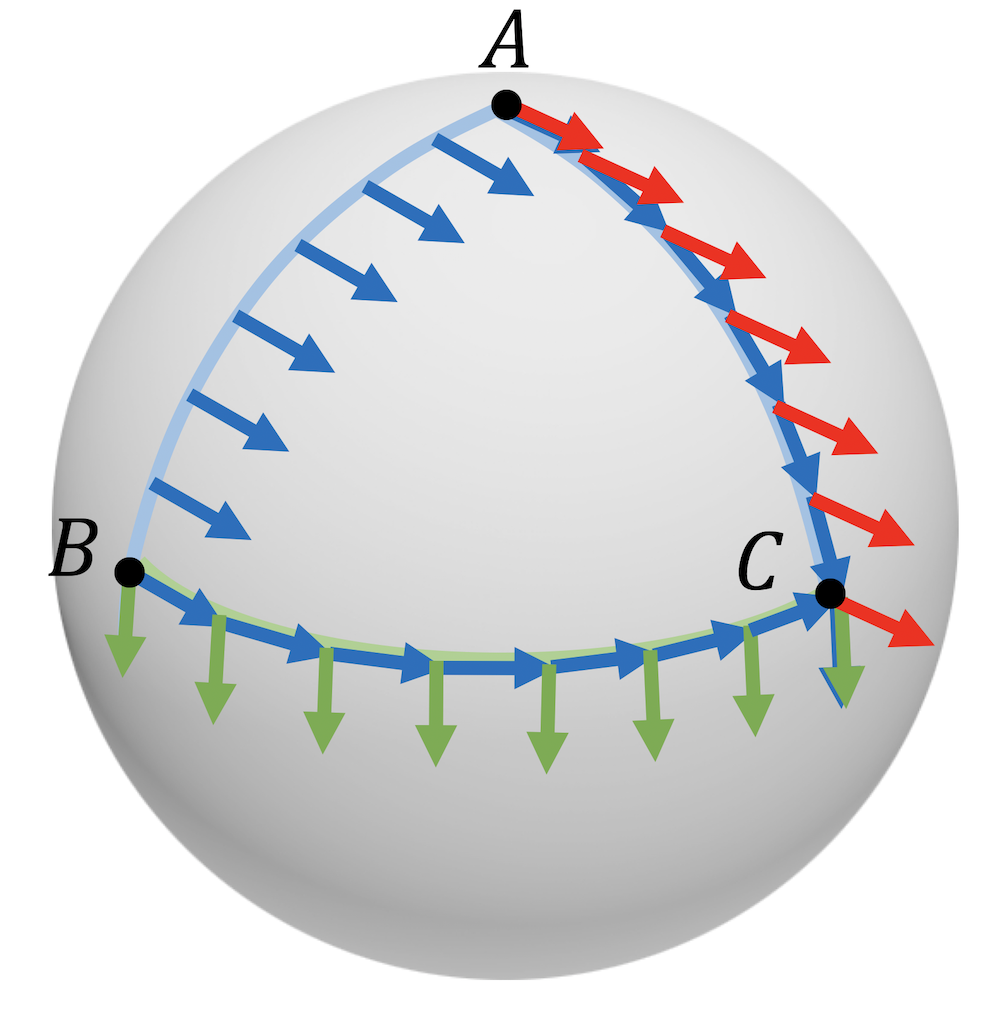
\includegraphics[width=0.9\linewidth]{figures/parallel.png}
%Euclidean transport of a vector from A to C makes no sense on the sphere, as the resulting vectors (red) are not in the tangent plane. Parallel transport from A to C (blue) rotates the vector along the path. It is path dependent: going along the path BC and ABC produces different results.  
%} (the derivative vanishes) for a small displacement along the curve. 
%%
%The result of the transport is path-dependent, which is best visualised on the sphere (see insert): moving a vector from the north pole to the equator along two different curves produces different results.
%%
%The name `connection' stems from the fact that parallel transport defines a linear isomorphism between tangent spaces along the curve $\gamma$, that is, a way to transport vectors from $T_{\gamma(0)}\Omega$ to $T_{\gamma(T)}\Omega$, thereby `connecting' these spaces.
%
%
%%which transports its tangent along itself 
%
%
%%perform  
%%of tangent vectors by (in this way, it ``connects'' two tangent spaces at different points, hence the alternative name `connection').  
%
%It is important to note that the definition of the covariant derivative  %and geodesic 
%does not rely on the metric, and  
%in fact, is an abstract construction that extends beyond Riemannian manifolds. %there are multiple ways to define one.  
%%
%When one is given a Riemannian metric, of particular interest is a special kind of covariant derivative called the {\em Levi-Civita connection}, after the Italian mathematician Tullio Levi-Civita who introduced the notion in 1917. %\marginnote{}
%%
%
%
%\begin{tcolorbox}[width=\linewidth,
%              boxsep=0pt,
%              left=7.5pt,
%              right=7.5pt,
%              top=7.5pt,
%              bottom=7.5pt,
%              arc=0pt,
%              boxrule=0pt,toprule=0pt,
%              colback=boxgray,
%              ]%%
%The {\em Levi-Civita connection} on a Riemannian manifold with metric $g$ is a connection $\nabla$ that additionally satisfies the following properties:
%\vspace{3mm}\\
%%\begin{enumerate}
%%\item 
%    \noindent  {\em Torsion free:} \marginnote{Roughly, {\em torsion} describes how tangent vectors twist about the curve when parallel transported, and {\em curvature} how they roll along it. }
%$\nabla_X Y - \nabla_Y X = [X,Y]$, where the tangent vector field $[X,Y] \in \mathcal{X}(\Omega, T\Omega)$ is the 
%{\em commutator} (also known as the {\em Lie bracket} or {\em Lie derivative}), defined by its action on scalar fields 
%$$[X,Y](z) = X(Y(z)) - Y(X(z)).$$
%%\vspace{2mm}\\
%%    
%\noindent {\em Preserves the metric:}\marginnote{Connection with this property is also known as {\em metric} or {\em metric-compatible}.} 
%$\nabla g = 0$, which is understood as 
%$$
%(\nabla_X g)(Y,Z) = X(g(Y,Z)) - g(\nabla_X Y, Z) - g(Y, \nabla_X Z) = 0.
%$$
%for any smooth $X, Y$, and $Z$. 
%
%\end{tcolorbox}
%
%
%%
%%
%The condition $\nabla g = 0$ (metric compability) implies that the metric remains invariant under parallel transport, i.e., parallel transport preserves the length of the tangent vectors (and is thus an isometry). 
%%
%The torsion-free properties make the Levi-Civita connection {\em unique}, a result known as the Fundamental Theorem of Riemannian Geometry. 
%%
%%\marginnote{
%For this reason, in Riemannian geometry the term `connection' is usually synonymous with the Levi-Civita connection, which can be considered a `canonical' connection.
%
%%guaranteeing that every Riemannian manifold admits a unique Levi-Civita connection, making it thus the `canonical' one. 
%
%
%
%
%%\taco{I think the notion of Torsion will be difficult to understand for newbies. Also, we are differentiating a tensor field g which I think we have not explained yet.
%
%%We could consider just mentioning the LC connection and explaining that parallel transport defined wrt it will not change the length of tangent vectors. We can also say that if another condition (Torsion free) is satisfied, there is a unique LC connection, without formalizing it.}
%
%
%
%\paragraph{Geodesics and Exponential map}
%
%A curve $\gamma$ along which parallel transport preserves the tangent vector to the curve,\marginnote{From the Greek \textgreek{geodai\textsigma{}{\'i}a}, literally `division of Earth'.}  i.e., $\nabla_{\gamma'} \gamma' = 0$ is called {\em geodesic}.
%%
%Locally at a point $u$, it is always possible to define a unique geodesic in a given direction $X$, i.e. a smooth curve $\gamma_X : [0,T] \rightarrow \Omega$ satisfying $\gamma(0) = u$ and $\gamma'(0) = X$, for some small $T>0$. 
%%
%%
%This\marginnote{Here, $B_r(0)$ is a ball of radius $r$ around the origin. Note that geodesic completeness does not necessarily guarantee that $\exp$ is a diffeomorphism -- the largest radius $r$ about $u$ for which $\exp_u(B_r(0) \subseteq T_u\Omega)$ is mapped diffeomorphically is called the {\em injectivity radius}. } gives a natural mapping from (a subset of) the tangent space $T_u \Omega$ to $\Omega$ called the {\em exponential map} $\exp : B_r(0) \subset T_u\Omega \rightarrow \Omega$, which is defined by taking a unit step along the geodesic in the direction $X$, i.e., $\exp_u(X) = \gamma_X(1)$. %
%%
%%
%When $\gamma_X(t)$ is defined for all $t\geq 0$ (that is, we can shoot the geodesic from a point $u$ for as long as we like), the manifold is said to be {\em geodesically complete} and the exponential map is defined on the whole tangent space.
%%
%Since compact manifolds are geodesically complete, we can tacitly assume this convenient property. 
%
%
%
%%
%On Riemannian\marginnote{It is tacitly assumed that curves are given in {\em arclength parametrisation}, such that $\| \gamma' \| = 1$ (constant velocity).} manifolds with the Levi-Civita connection, one can show geodesics to be {\em length-minimising curve}, 
%%
%i.e., a geodesic $\gamma$ minimises the length functional 
%%
%$$
%L(\gamma) = \int_{0}^T \| \gamma'(t) \| \mathrm{d}t =  \int_{0}^T g_u^{1/2} (\gamma'(t), \gamma'(t)) \mathrm{d}t 
%$$
%%
%among all curves with endpoints $u = \gamma(0)$ and $v=\gamma(T)$. 
%%
%%
%Readers familiar with metric geometry are probably more used to this definition of geodesics as shortests paths. 
%%
%In fact, \marginnote{Hopf-Rinow Theorem thus estabilishes the equivalence between geodesic and metric completeness, the latter meaning every Cauchy sequence converges.} a result known as the Hopf-Rinow Theorem guarantees that geodesically complete manifolds are also {\em complete metric spaces}, in which one can realise a metric (called the {\em geodesic distance})  between any pair of points $u,v$ as the length of the shortest path between them
%$$
%d_g(u,v) = \min_{\gamma} L(\gamma) \quad\quad \text{s.t.} \quad\quad \gamma(0) = u, \,\, \gamma(T) = v,
%$$
%which exists (i.e., the minimum is attained).\marginnote{To avoid confusion with the Riemannian metric, we will use the term `distance'. Our notation $d_g$ makes the distance depend on the Riemannian metric, though the definition of $L$. }
%%
%Importantly, geodesic distances are intrinsic, being dependent solely on the Riemannian metric. 
%
%
%%The term `geodesic' is also used in metric geometry, where it is defined as the shortest path. In the setting described here the two meanings coincide. }
%
%
%%i.e., the two notions of `geodesic' used somewhat differently in differential and metric geometry
%
%
%
%
%
%%===
%%
%%
%%For a smooth scalar field\marginnote{Linear functionals acting on vectors are called {\em dual vectors} or {\em covectors}. By the Riesz-Fr{\'e}chet Representation Theorem, every covector can be expressed as an inner product with a vector. } $x: \Omega \rightarrow \mathbb{R}$, the differential can be thought of as an operator $dx : T\Omega \rightarrow \mathbb{R}$ acting on tangent fields. At each point, the differential can be expressed as a linear functional acting on tangent vectors
%%$dx(u)  = g_u(\nabla x(u), \cdot)$. 
%%%
%%%
%%Given a smooth vector field $Y$, 
%%the {\em covariant derivative} $\nabla_Y x$ of $x$ {\em along} $Y$ is defined as 
%%$(\nabla_Y x)(u) = g_u(\nabla x(u), Y(u))$
%%and is a generalisation of the corresponding notion in classical calculus. 
%%%
%%%The change of the value of $x$ as the result of 
%%%displacement $y \in T_u\Omega$ at point $u$ is thus given by applying the form to the tangent
%%%vector, $dx(u) y = g_u(\nabla x(u), y)$, and can be thought
%%%of as an extension of the notion of the classical directional
%%%derivative.
%%%
%%The vector field $\nabla x$ is called the (intrinsic) {\em gradient} of $x$; at each point, it indicates the direction of the steepest increase of $x$. 
%%%
%%%The symbol $\nabla$ can be though of as an operator acting on scalar fields and producing vector fields defined above.  
%%
%%
%%Given two smooth vector fields $x$ and $y$, the covariant derivative $\nabla_y x$ of $x$ along $y$
%%
%%
%%
%%
%%Connection is defined as an abstract map $\nabla : T\Omega \times T\Omega \rightarrow T\Omega$ associating $(x,y) \mapsto \nabla_y x$ in a way that is linear w.r.t. both $x$ and $y$ and also satisfies the {\em product rule} $\nabla_y(xz) = x\nabla_y z + z \nabla_y x$ for any vector fields $x,y$ and scalar field $z$. 
%%
%%
%%
%%When the manifold is embedded in a Euclidean space, the covariant derivative coincides with the standard Euclidean directional derivarive projected onto the tangent space. 
%%
%%
%%
%%
%%
%%
%%%known as the {\em pushforward} $d\eta : T\Omega \rightarrow T\Omega'$.  
%%
%%
%%
%%the notion of derivative describes how the value of a function changes with an infinitesimal change of its
%%argument. 
%%
%%
%%One of the big differences distinguishing classical
%%calculus from differential geometry is a lack of vector space
%%
%%
%%structure on the manifold, prohibiting us from na\"{i}vely using
%%expressions like $f(x+dx)$. The conceptual leap that is required
%%to generalize such notions to manifolds is the need to work
%%locally in the tangent space
%%
%%
%%
%%
%%
%%
%%
%%
%%
%%
%
%
%
%
%
%\paragraph{Isometries}
%Consider now a deformation of our manifold $\Omega$ into another manifold $\Omega'$ with a Riemannian metric $h$.
%%
%We will assume this map to be a diffeomorphism $\eta: (\Omega, g) \rightarrow (\Omega', h)$ between manifolds.   
%%
%Its differential $\mathrm{d}\eta : T\Omega \rightarrow T\Omega'$ defines a map between the respective tangent bundles (referred to as {\em pushforward}), such that   
%%\marginnote{The pushforward is what is called a {\em bundle map}.}
%at a point $u$, we have $\mathrm{d}\eta_u : T_u \Omega \rightarrow T_{\eta(u)}\Omega'$, %which allows to interpret it as follows: 
%%
%interpreted as before: 
%if we make a small displacement from point $u$ by tangent vector $X \in T_u \Omega$, the map $\eta$ will be displaced from point $\eta(u)$ by tangent vector $\mathrm{d}\eta_u(X) \in T_{\eta(u)}\Omega'$. 
%
%
%Since the pushforward provides a mechanism to associate tangent vectors on the two manifolds, it allows to {\em pullback }\marginnote{Pushforward and pullback are adjoint operators $\langle \eta^* \alpha, X \rangle = \langle \alpha, \eta_*X \rangle$ where $\alpha \in T^*\Omega$ is a {\em dual vector field}, defined at each point as a linear functional acting on $T_u\Omega$ and the inner products are defined respectively on vector and dual vector fields. } the metric $h$ from $\Omega'$ to $\Omega$, 
%$$
%(\eta^*h)_u(X,Y) = h_{\eta(u)}(\mathrm{d}\eta_u(X), \mathrm{d}\eta_u(Y))
%$$ 
%%
%If the pullback metric coincides at every point with that of $\Omega$, i.e., $g = \eta^*h$, the map $\eta$ is called  (a Riemannian) {\em isometry}. % (metric-preserving). 
%%
%For two-dimensional manifolds (surfaces), isometries can be intuitively understood as inelastic deformations that deform the manifold without `stretching' or `tearing' it. 
%
%
%
%By virtue of their definition, isometries preserve intrinsic structures such as geodesic distances, which are expressed entirely in terms of the Riemannian metric. % and Gaussian curvature.
%%
%Therefore, we can also understand isometries from the position of metric geometry,\marginnote{The Myers–Steenrod Theorem establishes that the converse is also true on connected manifolds: every metric isometry is also a Riemannian isometry. } 
%as distance-preserving maps {\em between metric spaces} $\eta : (\Omega, d_g) \rightarrow (\Omega', d_h)$, in the sense that 
%$$
%d_g (u,v) = d_h(\eta(u),\eta(v)) 
%$$
%for all $u,v \in \Omega$, 
%or more compactly, $d_g = d_h \circ (\eta \times \eta)$. 
%%where $d_g, d_g$ are the geodesic distances induced by the respective Riemannian metrics $g, h$. 
%%
%
%%[Gauss Theorema Egregium, definition of curvature through perimeter defect, pizza example]
%
%
%A particular case of the above is a diffeomorphism  of the domain itself, which we will denote by $\tau \in \mathrm{Diff}(\Omega)$. We will call it a Riemannian  \mbox{(self-)isometry} if the pullback metric satisfies $\tau^* g = g$, or a metric (self-)isometry if $d_g = d_g\circ (\tau \times \tau)$.
%%
%Not surprisingly, isometries form a group with the composition operator denoted by $\mathrm{Iso}(\Omega)$ and called the {\em isometry group}; the identity element is the map $\tau(u) = u$ and the inverse always exists (by definition of $\tau$ as a diffeomorphism). 
%%
%Self-isometries are thus {\em intrinsic symmetries} of manifolds.
%
%
%%Continuous symmetries on manifolds are infinitesimally generated
%%%\marginnote{More correctly, Killing fields are the infinitesimal generators of continuous symmetries. } 
%%by special tangent vector fields called {\em Killing fields}, named after Wilhelm Killing. A field $X$ is Killing if the  Lie derivative\marginnote{The Lie derivative in this case is a derivative of forms. For scalar and vector fields, it coincides with the covariant derivative $\mathcal{L}_X y = \nabla_X y$ and the commutator $\mathcal{L}_X Y = [X,Y]$, respectively. } of the Riemannian metric along it vanishes, $\mathcal{L}_X g = 0$, which is interpreted as 
%%%
%%$$
%%\mathcal{L}_X g(Y,Z) = g(\nabla_Y X, Z) + g(Y,\nabla_Z X) = 0
%%$$
%%for any smooth tangent fields $Y, Z$. 
%%%
%%We can recap that like we mentioned in Section~\ref{sec:symmetries}, we can regard symmetries as automorphisms (self-maps) preserving additional structure: either the local Riemannian metric, or global geodesic distances between pairs of points. 
%%%\taco{Do we need Killing fields? It's interesting but I worry that we'd need to properly introduce Lie derivatives to make it understandable.} \michael{Lets keep them for now}
%%%OK :)
%



\paragraph{Riemann 流形}
\label{sec:manifolds}

由于流形的形式定义\marginnote{“光滑”是指可微足够多次；为方便起见，我们默认采用这一假设。这里的“形变”是指\emph{微分同胚}，即两个邻域之间存在光滑可逆映射，且其逆映射也光滑。%, called a diffeomorphism.
%In this way, we can choose smooth coordinates for neighbourhoods of the manifold.
}较为复杂，我们
%defer its detailed discussion to Chapter ??? and 
宁愿牺牲一些精确性，给出直观图景。
%
在这里，可以把（可微或光滑）流形看作一个光滑的多维弯曲曲面%(or higher dimensional space)
，它\emph{局部 Euclidean}；也就是说，任意一点附近的任意小邻域都可以形变为
%\marginnote{`Deformed' here means \emph{homeomorphic to}, i.e. we can map between the neighbourhoods using a continuous and invertible map with continuous inverse. In fact, we will assume the manifold is smooth, in which case the map should be a diffeomorphism -- smooth and invertible with smooth inverse.}
一个 $\R^s$ 的邻域；
%A crucial difference between a manifold\marginnote{We also tacitly assume the manifold to be smooth, i.e. having a $\mathcal{C}^\infty$-differentiable set of transition functions between local spaces.} and a Euclidean space is that a manifold is only {\em locally} Euclidean:  %
%a small neighbourhood (open set) around each point $u \in \Omega$ is homeomorphic 
%\marginnote{A {\em homeomorphism} is a continuous map with continuous inverse that preserves topological properties.}  to 
%(topologically equivalent) to $\mathbb{R}^s$; 
%
%by a homeomorphism called a {\em chart}; 
%the dimension $d$ is that of the manifold, which 
此时称该流形是 $s$-{\em 维的}。
%
%The composition of two charts (or more precisely, a chart and an inverse of a chart) allows to transition between the local 
%
%
%Since the manifold is smooth, 
这使我们能够
局部近似点 $u$ 附近的流形，所使用的是\emph{切空间} $T_u\Omega$。%and called the {\em tangent space}.
可以通过一个典型二维流形——球面——来直观理解切空间：在球面上一点附着一个平面；充分放大后，球面会显得像平面（图~\ref{fig:sphere_metric}）。
% This analogy however should not be taken literally, as manifolds are abstract objects existing on their own without any geometric realization.  % Taco: this may be a bit confusing for newbies
%
\marginnote{形式上，切丛是{\em 不交并} $\displaystyle T\Omega = \bigsqcup_{u\in \Omega} T_u\Omega$。}所有切空间的集合称为{\em 切丛}，记为 $T\Omega$；第~\ref{sec:gauges} 节将更详细地讨论丛的概念。
%later and also in Chapter ???.



{\em 切向量}记为 $X\in T_u\Omega$，可以把它理解为从点 $u$ 出发的局部位移。
%In order to give it a sense of {\em direction}, 
为了测量切向量的\emph{长度}及其夹\emph{角}，%, and {\em volumes},
%
\marginnote{若双线性函数 $g$ 对任意非零向量都满足 $g(X,X)>0$，其中 $X\neq 0$，则称其{\em 正定}。若把 $g$ 表示为矩阵 $\mathbf{G}$，则这意味着 $\mathbf{G} \succ 0$。行列式 $|\mathbf{G}|^{1/2}$ 给出一个与基的选择无关的局部体积元素。}
%
需要为切空间配备附加结构，该结构表示为
正定双线性函数
$g_u: T_u\Omega \times T_u\Omega \rightarrow \mathbb{R}$，并光滑依赖于 $u$。这类函数
称为{\em Riemann 度量}，以纪念 1856 年引入这一概念的 Bernhardt Riemann；它可以看作切空间上的内积 $\langle X, Y \rangle_u = g_u(X,Y)$，表达任意两个切向量 $X, Y \in T_u\Omega$ 之间的夹角。
%
该度量还诱导范数 $\| X \|_u = g_u^{1/2}(X,X)$，从而能够局部测量向量长度。



必须强调，切向量
是独立存在的抽象几何实体，并且{\em 不依赖坐标}。若要以数值数组表示切向量 $X$，只能把它表示成{\em 相对于某个局部基}的一列坐标 $\mathbf{x}=(x_1, \hdots, x_s)$。\marginnote{遗憾的是，人们常常把向量与其坐标等同起来。
%, which in our view constitutes a crime against humanity. 
为强调这一重要区别，我们用 $X$ 表示切向量，用 $\mathbf{x}$ 表示其坐标。}该局部基为 $\{ X_1, \hdots X_s \} \subseteq T_u\Omega$。
%
类似地，在该基下，度量可以表示为 $s\times s$ 矩阵 $\mathbf{G}$，其元素为 $g_{ij} = g_u(X_i,X_j)$。
%
第~\ref{sec:gauges} 节将回到这一点。
%; however, we stress that the definition of Riemannian metric does not rely on any particular choice of basis %all our definitions are coordinate-free and exist independently of any basis choice
%(this will be the centrepiece of the following section). 

%that allows to measure length, angle, and volume in the tangent space. 
%

%\michael{Add a simple example here}


\begin{figure}[h!]
    \centering
    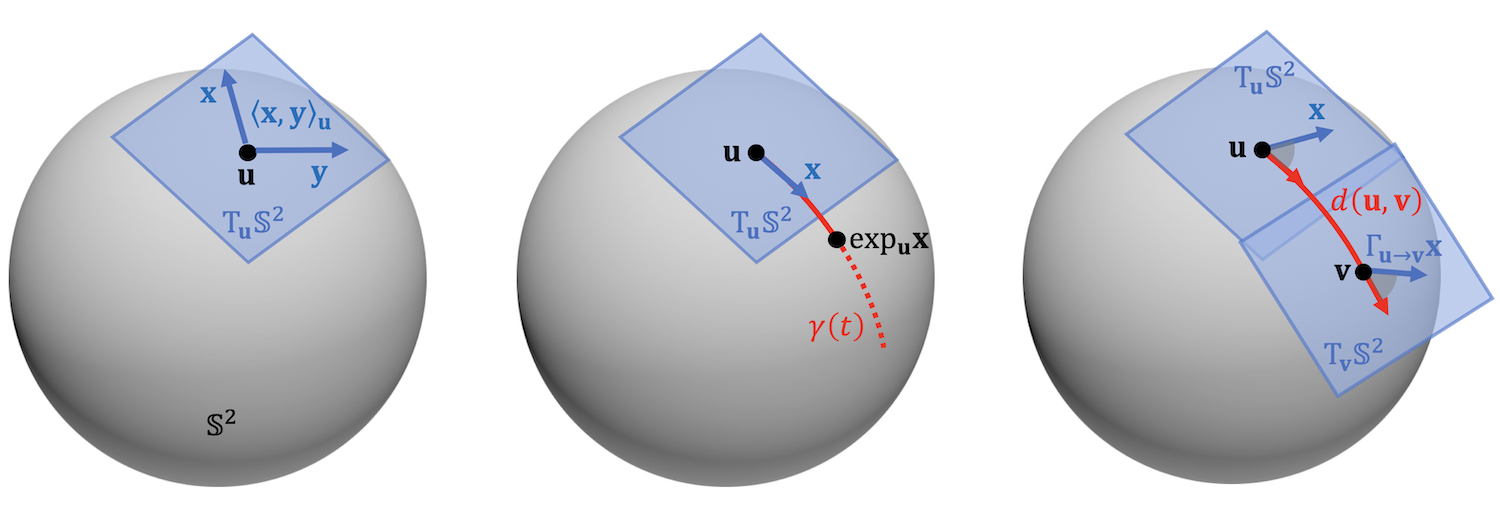
\includegraphics[width=\linewidth]{figures/manifold.png}
    \caption{
    以二维球面 $\mathbb{S}^2 = \{\mathbf{u}\in \mathbb{R}^3 : \|\mathbf{u}\|=1 \}$ 为例说明 Riemann 几何的基本概念；该球面实现为 $\mathbb{R}^3$ 的子集（子流形）。
%
球面的切空间为 $T_\mathbf{u}\mathbb{S}^2 = \{ \mathbf{x}\in \mathbb{R}^3 : \mathbf{x}^\top \mathbf{u} = 0\}$，它是二维平面，因此球面是二维流形。Riemann 度量就是限制在切平面上的 Euclidean 内积，即 $\langle \mathbf{x}, \mathbf{y}\rangle_\mathbf{u} = \mathbf{x}^\top \mathbf{y}$，对任意 $\mathbf{x},\mathbf{x}\in T_\mathbf{u}\mathbb{S}^2$ 成立。
指数映射为
$\exp_\mathbf{u}(\mathbf{x}) = \cos(\| \mathbf{x}\|)\mathbf{u} + \frac{\sin(\| \mathbf{x}\|)}{\|\mathbf{x}\|} \mathbf{x}$，其中 $\mathbf{x} \in T_\mathbf{u}\mathbb{S}^2$。
%
测地线是长度为 $d(\mathbf{u},\mathbf{v}) = \cos^{-1}(\mathbf{u}^\top \mathbf{v})$ 的大圆弧。
    }
    \label{fig:sphere_metric}
\end{figure}%


%an {\em inner product}.
%In differential geometry, an inner product on $T_u\Omega$ depending smoothly on $u$ is called a {\em Riemannian metric}, in honour of Bernhardt Riemann who introduced the concept in 1856. %
%We will denote a Riemannian metric as a$g_u: T_u\Omega \times T_u\Omega \rightarrow \mathbb{R}$ that allows to measure length, angle, and volume in the tangent space. 
%

%
%of a vector $$
%
%angle between two tangent vectors $x,y \in T_u\Omega$, (expressed %as $\cos^{-1}\left( \frac{\g_u(x,y)$) and a length of the 


配备度量的流形称为
{\em Riemann 流形}，完全能够用度量表达的性质称为{\em 内蕴性质}。%
这是本书讨论中的关键概念，因为按照我们的模板，将寻求构造作用于 $\Omega$ 上所定义信号的函数，使其对保持度量的变换具有不变性。这类变换称为{\em 等距变换}，它们使流形发生形变而不影响其局部结构。\marginnote{

\includegraphics[width=1\linewidth]{figures/origami.pdf}
这一结果称为{\em 嵌入定理}，由
\cite{nash1971imbedding}.
%John Forbes Nash, who became a household name after the Hollywood movie The Beautiful Mind. 
折纸%paper folding
艺术体现了平面曲面在 $\mathbb{R}^3$ 中的不同等距嵌入（图片：Shutterstock/300 librarians）。
}如果这类函数能够用内蕴量表达，就会自动保证等距不变性，从而不受等距形变影响。
%
这些结果还可以进一步推广到近似等距变换；因而这是蓝图中所讨论几何稳定性（域形变）的一个实例。


%\taco{Taco: here we should probably make clear that we are not talking about symmetries in the sense of automorphisms, i.e. maps $\Omega \rightarrow \Omega$ that preserve the metric, but about isomorphisms, i.e. maps $\Omega \rightarrow \Omega'$ that preserve the metric. Note that we do not yet discuss this in the template, but as discussed we should.} 

%\michael{Approx isometry - geometric stability}

正如前面所指出的，Riemann 流形的定义不要求它
在任何空间中具有几何实现；但事实证明，任意光滑 Riemann 流形都可以实现为足够高维 Euclidean 空间的子集（此时称它“嵌入”该空间），并利用 Euclidean 空间的结构诱导 Riemann
度量。不过，这类嵌入未必唯一——正如下文将看到的，同一个 Riemann 度量可以具有两个不同的等距
实现。
%called {\em isometries}.



%\joan{Consider a transition paragraph here, where we explain that we introduce the minimal elements of differential geometry that lead to the key notion of isometry and geodesics}



\paragraph{标量场与向量场}
%
由于我们关心定义在 $\Omega$ 上的信号，需要给出流形上标量值
%\marginnote{We will use the same notation for tangent and vector fields, the distinction between which will be clear from the context.} 
与向量值函数的恰当概念。
%
（光滑）{\em 标量场}是形如 $x: \Omega\rightarrow \mathbb{R}$ 的函数。\marginnote{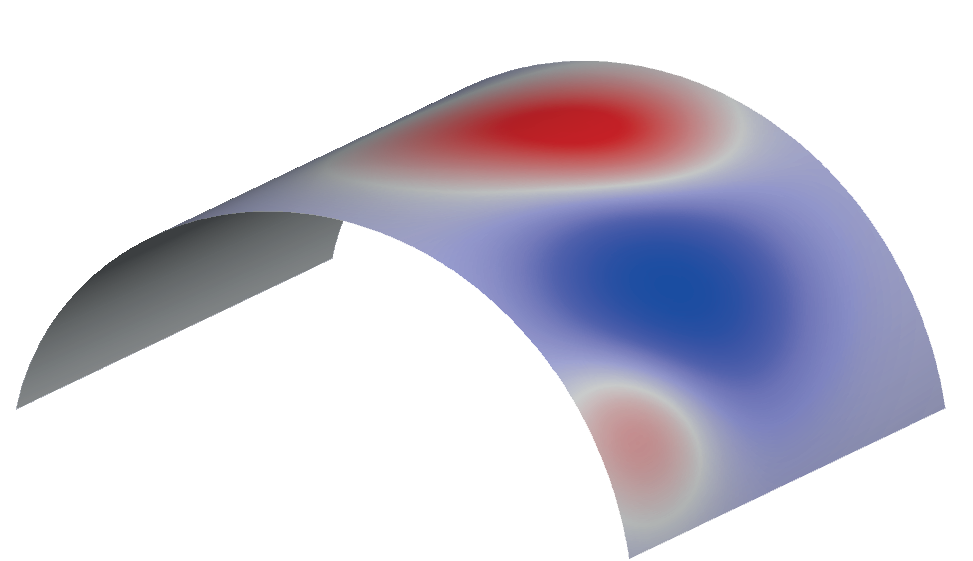
\includegraphics[width=0.9\linewidth]{figures/field_scalar.pdf}\\
标量场示例。
}
%\marginnote{The fields are typically assumed to be of the same regularity class (smoothness) as the manifold itself. }
%
%scalar-valued function  (often called a {\em scalar field}) $x: \Omega\rightarrow \mathbb{R}$ on the manifold. The space of 
标量场构成向量空间 $\mathcal{X}(\Omega, \mathbb{R})$，该空间可以配备内积%of scalar fields
\begin{equation}
\langle x, y \rangle = \int_\Omega x(u) y(u) \mathrm{d}u,
\label{eq:inner_scalar}   
\end{equation}
%
其中 $\mathrm{d}u$ %= \sqrt{\det g}$
%\marginnote{More rigorously speaking, the volume form requires an inner product (i.e. Riemannian metric) and {\em orientation} (`handedness'). } 
是由 Riemann 度量诱导的体积元素。
%
%
（光滑）{\em 切向量场}是形如 $X: \Omega \rightarrow T\Omega$ 的函数，它为每个点指定相应切空间中的一个切向量，即 $u\mapsto X(u)\in T_u\Omega$。
%
向量场\marginnote{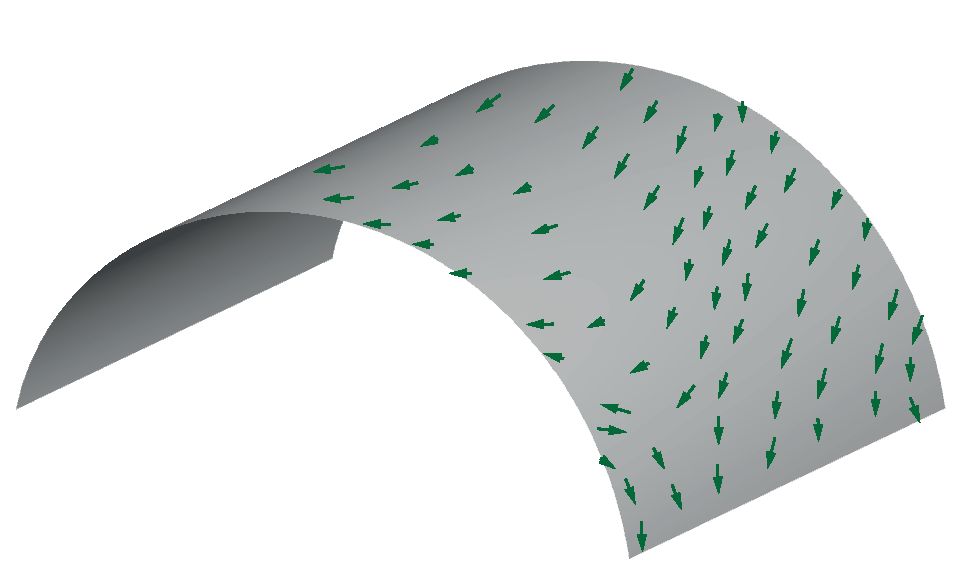
\includegraphics[width=0.9\linewidth]{figures/field_vector.pdf}\\
向量场示例。通常假设场与流形本身具有相同的正则性类别（光滑度）。
}也构成向量空间 $\mathcal{X}(\Omega, T\Omega)$，其内积由 Riemann 度量定义：
%
\begin{equation}
\langle X, Y \rangle = \int_\Omega g_u(X(u), Y(u)) \mathrm{d}u. \label{eq:inner_vector}   
\end{equation}


\paragraph{内蕴梯度}
理解（并实际{\em 定义}）向量场的另一种方式，是把它视为导数概念的推广。
%
在经典微积分中，可以通过{\em 微分} $\mathrm{d}x(u) = x(u+\mathrm{d}u) - x(u)$ 对（光滑）函数作局部线性化；它给出函数 $x$ 在点 $u$ 处因无穷小位移 $\mathrm{d}u$ 而发生的值变化。
%
然而，在本情形下无法直接套用这一定义，因为
%brings up two problems: First, 
由于缺乏全局向量空间结构，形如“$u+\mathrm{d}u$”的表达式在流形上没有意义。
%, preventing us from adding or subtracting two points on $\Omega$. 
%
%
%A second problem arises when trying to take derivatives of vector fields, as one would need to subtract vectors belonging to tangent spaces at {\em different points}, while subtraction is only define \emph{within} a single vector space. 





解决办法是%to the first problem is
用切向量对局部无穷小位移建模。
%in order to provide a proper generalization of the differential on manifolds. 
%
给定光滑标量场 $x\in \mathcal{X}(\Omega,\mathbb{R})$，可以把（光滑）向量场视为满足{\em 导子}性质的线性映射 $Y:\mathcal{X}(\Omega,\mathbb{R}) \rightarrow \mathcal{X}(\Omega,\mathbb{R})$：
$Y(c) = 0$ 对任意常数 $c$ 成立（对应于常数函数的导数为零这一直觉）；$Y(x+z) = Y(x) + Y(z)$（线性性）；以及 $Y(xz) = Y(x)z + xY(z)$（{\em 乘积法则}或 {\em Leibniz 法则}）。这些性质对任意光滑标量场 $x,z \in \mathcal{X}(\Omega,\mathbb{R})$ 均成立。
%
可以证明，能够利用这些性质公理化地定义向量场。
%
微分 $\mathrm{d}x(Y) = Y(x)$
可以视为算子 $(u,Y) \mapsto Y(x)$，
%
%defined as an operator $\mathrm{d}x : T\Omega \rightarrow \mathbb{R}$ of the form
%$$
%\mathrm{d}x(Y) = Y(x),
%$$
%which can be 
其解释如下：$x$ 因位移 $Y \in T_u\Omega$ 在点 $u$ 处而发生的变化，由 $\mathrm{d}_ux(Y)$ 给出。\marginnote{重要的是，这一构造{\em 完全不使用 Riemann 度量}，因此可以推广到第~\ref{sec:gauges} 节所讨论的更一般丛构造。}
%
因此，它是经典{\em 方向导数}概念的推广。
%



另一种观点是，在每个点 $u$ 处，可以把微分视为{\em 线性泛函} $\mathrm{d}x_u : T_u\Omega \rightarrow \mathbb{R}$，它作用于切向量 $X \in T_u\Omega$。向量空间上的线性泛函称为{\em 对偶向量}或{\em 余向量}；若还给定内积（Riemann 度量），则对偶向量总可以表示为
$$
\mathrm{d}x_u (X)  = g_u(\nabla x(u), X).\marginnote{This is a consequence of the Riesz-Fr{\'e}chet Representation Theorem, by which every dual vector can be expressed as an inner product with a vector. } 
$$ 
点 $u$ 处微分的表示是切向量 $\nabla x(u) \in T_u \Omega$，称为 $x$ 的（内蕴）{\em 梯度}；与经典微积分中的梯度类似，可以把它理解为 $x$ 增长最快的方向。
%
把梯度视为{\em 算子} $\nabla : \mathcal{X}(\Omega,\mathbb{R}) \rightarrow \mathcal{X}(\Omega,T\Omega)$ 时，它在每个点指定 $x(u) \mapsto \nabla x(u) \in T_u \Omega$；因此，标量场 $x$ 的梯度是向量场 $\nabla x$。
%As we will see later, this construction will allow us to generalise the notion of Fourier transform to manifolds. 

%More generally, the gradient can be thought of as an operator $\nabla : $



%In other words, the gradient produces a tangent vector field indicating the local direction of steepest increase of a scalar field on the manifold. 





%\taco{I think the notion of Torsion will be difficult to understand for newbies. Also, we are differentiating a tensor field g which I think we have not explained yet.

%We could consider just mentioning the LC connection and explaining that parallel transport defined wrt it will not change the length of tangent vectors. We can also say that if another condition (Torsion free) is satisfied, there is a unique LC connection, without formalizing it.}



\paragraph{测地线}

现在考虑流形上的光滑曲线 $\gamma : [0,T] \rightarrow \Omega$，其端点为 $u = \gamma(0)$ 和 $v = \gamma(T)$。曲线在点 $t$ 处的导数是切向量 $\gamma'(t) \in T_{\gamma(t)}\Omega$，称为{\em 速度向量}。\marginnote{默认假设曲线采用{\em 弧长参数化}，使得 $\| \gamma' \| = 1$（速度恒定）。}
%
在连接点 $u$ 与 $v$ 的所有曲线中，我们关心{\em 长度最短}的曲线，即寻找使长度泛函最小的 $\gamma$：
%
$$
\ell(\gamma) = \int_{0}^T \| \gamma'(t) \|_{\gamma(t)} \mathrm{d}t =  \int_{0}^T g_{\gamma(t)}^{1/2} (\gamma'(t), \gamma'(t)) \mathrm{d}t. 
$$
%
这类曲线称为{\em 测地线}（源自希腊语 \textgreek{geodai\textsigma{}{\'i}a}，字面意为“划分地球”），在微分几何中起着重要作用。
%
%
对本书讨论至关重要的是，我们对测地线的定义是内蕴的，因为它们只依赖 Riemann 度量（通过长度泛函）。


熟悉微分几何的读者可能记得，测地线是一个更一般的概念，其定义实际上未必需要 Riemann 度量，而只需要{\em 联络}（也称为{\em 协变导数}，因为它把导数概念推广到向量场和张量场）；联络与前面对微分的构造类似，以公理方式定义。
%
给定 Riemann 度量，存在唯一的特殊联络，称为\marginnote{Levi-Civita 联络无挠且与度量相容。Riemann 几何基本定理保证其存在性与唯一性。}{\em Levi-Civita 联络}；Riemann 几何通常默认使用该联络。由这一联络产生的测地线，就是上面定义的长度最短曲线。


下面将说明如何利用测地线定义在流形上传输切向量的方式（平行输运），建立从流形到切空间的局部内蕴映射（指数映射），并定义距离（测地度量）。这将允许我们通过在切空间中局部应用滤波器，构造类似卷积的运算。%
%among all curves with endpoints $u = \gamma(0)$ and $v=\gamma(T)$. 



\paragraph{平行输运}\marginnote{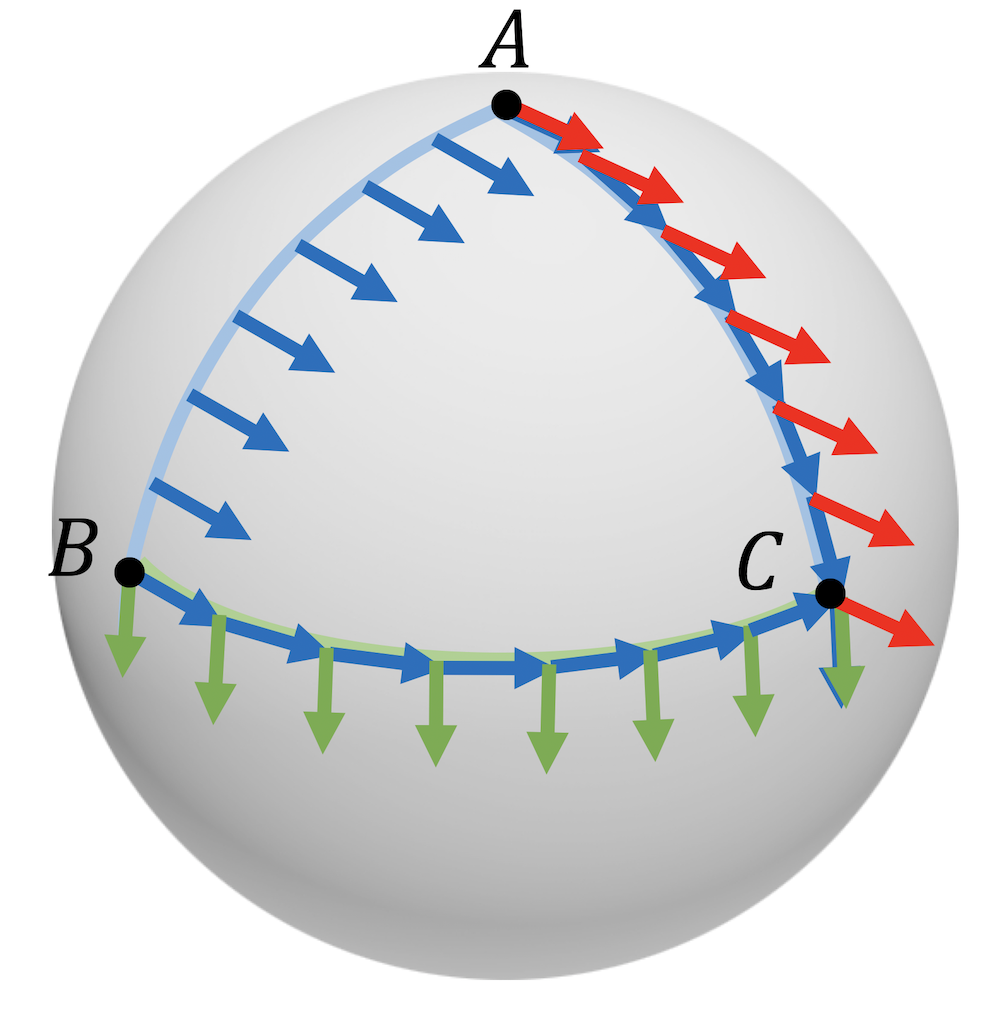
\includegraphics[width=0.9\linewidth]{figures/parallel.png}
在球面上，把向量从 A Euclidean 式地传输到 C 没有意义，因为所得向量（红色）不在切平面内。从 A 到 C 的平行输运（蓝色）沿路径旋转向量。它依赖于路径：沿 BC 与 ABC 路径输运会产生不同结果。
}
处理流形时已经遇到一个问题：不能直接对两点 $u,v \in \Omega$ 作加减运算。
%
比较不同点处的切向量时也会出现同样的问题：尽管维数相同，它们却属于{\em 不同空间}，例如 $X\in T_u\Omega$ 和 $Y\in T_v\Omega$，因而不能直接比较。
%
测地线提供了一种把向量从一点移动到另一点的机制，具体如下：令 $\gamma$ 为连接点 $u=\gamma(0)$ 与 $v=\gamma(T)$ 的测地线，并令 $X \in T_u\Omega$。可以沿测地线定义一组新的切向量 $X(t) \in T_{\gamma(t)}\Omega$，使 $X(t)$ 的长度以及它与曲线速度向量之间的夹角（由 Riemann 度量表示）保持不变：
$$
g_{\gamma(t)}(X(t),\gamma'(t) ) = g_{u}(X,\gamma'(0)) = \mathrm{const}, \quad\quad \|X(t)\|_{\gamma(t)} = \|X\|_u = \mathrm{const}.
$$
于是，在终点处得到唯一向量 $X(T) \in T_{v}\Omega$，该终点为 $v$。%, which is unique.


用上述记号定义的映射 $\Gamma_{u\rightarrow v}(X) : T_u\Omega \rightarrow T_u\Omega$ 和 $T_v\Omega$，即 $\Gamma_{u\rightarrow v}(X) = X(T)$，称为{\em 平行输运}或{\em 联络}；后一个术语意味着它是在切空间 $T_u\Omega$ 与 $T_v\Omega$ 之间建立“联结”的机制。
%
由于保持角度和长度，平行输运只相当于旋转向量，因此可与特殊正交群 $\mathrm{SO}(s)$ 的一个元素相关联（该群称为切丛的{\em 结构群}）。\marginnote{这里假设流形可定向，否则应为 $\mathrm{O}(s)$。}我们把该元素记为 $\fg_{u\rightarrow v}$，并将在第~\ref{sec:gauges} 节更详细地讨论。

如前所述，联络可以独立于 Riemann 度量以公理方式定义，从而给出沿任意光滑曲线进行平行输运的抽象概念。不过，这类输运的结果取决于所取路径。
%As a general comment, parallel transport can be defined along any cur

%or {\em connection} 




\paragraph{指数映射}
在点 $u$ 的局部，总能沿给定方向 $X \in T_u\Omega$ 定义唯一测地线，即满足%a smooth curve $\gamma_X : [0,T] \rightarrow \Omega$ satisfying
$\gamma(0) = u$ and $\gamma'(0) = X$. %, for some small $T>0$. 
%
%
当 $\gamma_X(t)$ 对所有 $t\geq 0$ 都有定义时（即可以从点 $u$ 出发把测地线延伸任意长），称流形{\em 测地完备}，且指数映射定义在整个切空间上。
%
由于紧致流形是测地完备的，可以默认采用这一便利性质。



%
这种由一点和一个方向定义测地线的方式，给出了从切空间 $T_u \Omega$（的一个子集）到 $\Omega$ 的自然映射，称为{\em 指数映射}。\marginnote{
%Here, $B_\delta(0)$ is a ball of radius $\delta$ around the origin. 
注意，测地完备性未必保证 $\exp$ 是全局微分同胚——最大半径 $r$ 以 $u$ 为中心，并使 $\exp_u(B_r(0) \subseteq T_u\Omega)$ 保持微分同胚映射；该半径称为{\em 单射半径}。}该映射为 $\exp : B_r(0) \subset T_u\Omega \rightarrow \Omega$，其定义是在方向 $X$ 上沿测地线前进一步，即 $\exp_u(X) = \gamma_X(1)$。%
%
指数映射 $\exp_u$ 是局部微分同胚，因为它把 $B_r(0)$（半径为 $r$ 的球，即 $T_u\Omega$ 中原点的邻域）形变为 $u$ 的一个邻域。反过来，也可以把指数映射视为流形到切空间的内蕴局部形变（“展平”）。




\paragraph{测地距离}
%
称为 Hopf-Rinow 定理的结果
%
\marginnote{因此，Hopf-Rinow 定理建立了测地完备性与度量完备性的等价性；后者意味着每个 Cauchy 序列都在测地距离度量下收敛。}保证测地完备流形也是{\em 完备度量空间}；在这样的空间中，任意点对 $u,v$ 之间的距离（称为{\em 测地距离}或{\em 度量}）都可以实现为连接两点的最短路径长度：
$$
d_g(u,v) = \min_{\gamma} \ell(\gamma) \quad\quad \text{s.t.} \quad\quad \gamma(0) = u, \,\, \gamma(T) = v,
$$
该路径存在（即最小值能够取到）。\marginnote{注意，“度量”一词有两种含义：Riemann 度量 $g$ 与距离 $d$。为避免混淆，指后者时将使用“距离”一词。记号 $d_g$ 表明距离依赖于 Riemann 度量 $g$，这种依赖通过测地长度 $L$ 的定义实现。}



%The term `geodesic' is also used in metric geometry, where it is defined as the shortest path. In the setting described here the two meanings coincide. }


%i.e., the two notions of `geodesic' used somewhat differently in differential and metric geometry







\paragraph{等距变换}
现在考虑把流形 $\Omega$ 形变为另一个流形 $\tilde{\Omega}$，后者配备 Riemann 度量 $h$；我们假设该形变是
%
%We will assume this map to be 
流形之间的微分同胚 $\eta: (\Omega, g) \rightarrow (\tilde{\Omega}, h)$。
%
其微分 $\mathrm{d}\eta : T\Omega \rightarrow T\tilde{\Omega}$ 定义了相应切丛之间的映射（称为{\em 前推}），使得
%\marginnote{The pushforward is what is called a {\em bundle map}.}
在点 $u$ 处有 $\mathrm{d}\eta_u : T_u \Omega \rightarrow T_{\eta(u)}\tilde{\Omega}$，%which allows to interpret it as follows:
%
其解释与前面类似：
如果用切向量从点 $u$ 作一个小位移，所用切向量为 $X \in T_u \Omega$，那么映射 $\eta$ 将从点 $\eta(u)$ 沿切向量 $\mathrm{d}\eta_u(X) \in T_{\eta(u)}\tilde{\Omega}$ 位移。


由于前推\marginnote{前推与拉回是伴随算子 $\langle \eta^* \alpha, X \rangle = \langle \alpha, \eta_*X \rangle$，其中 $\alpha \in T^*\Omega$ 是{\em 对偶向量场}，在每一点定义为作用于 $T_u\Omega$ 的线性泛函；两个内积分别定义在向量场和对偶向量场上。}提供了关联两个流形上切向量的机制，因而可以把度量 $h$ 从 $\tilde{\Omega}$ {\em 拉回}到 $\Omega$：
$$
(\eta^*h)_u(X,Y) = h_{\eta(u)}(\mathrm{d}\eta_u(X), \mathrm{d}\eta_u(Y))
$$ 
%
如果拉回度量在每一点都与 $\Omega$ 的度量一致，即 $g = \eta^*h$，则映射 $\eta$ 称为（Riemann）{\em 等距变换}。% (metric-preserving).
%
对于二维流形（曲面），等距变换可以直观地理解为非弹性形变：它使流形发生形变，却不“拉伸”或“撕裂”流形。



根据定义，等距变换保持测地距离等内蕴结构，而这些结构完全由 Riemann 度量表达。% and Gaussian curvature.
%
因此，也可以从度量几何的视角理解等距变换，
把它看作{\em 度量空间之间}保持距离的映射（“度量等距”）$\eta : (\Omega, d_g) \rightarrow (\tilde{\Omega}, d_h)$，即
$$
d_g (u,v) = d_h(\eta(u),\eta(v)) 
$$
对所有 $u,v \in \Omega$ 均成立，
更紧凑地写为 $d_g = d_h \circ (\eta \times \eta)$。换言之，Riemann 等距变换也是度量等距变换。
%
在{\em 连通}流形上，反之亦然：每个度量等距变换也是 Riemann 等距变换。
\marginnote{这一结果称为 Myers–Steenrod 定理。我们默认假设所讨论的流形是连通的。}
%where $d_g, d_g$ are the geodesic distances induced by the respective Riemannian metrics $g, h$. 


在几何深度学习蓝图中，$\eta$ 是域形变的模型。当 $\eta$ 为等距变换时，%(roughly, an inelastic deformation that does not `stretch' the manifold),
任何内蕴量都不受这类形变影响。
%
%This is the reason why we insist on working with structures defined intrinsically. 
%
可以通过下述概念推广精确的（度量）等距变换：%this notion
{\em 度量伸缩}
$$
\mathrm{dil}(\eta) = \sup_{u\neq v \in \Omega}\frac{d_h(\eta(u),\eta(v))}{d_g (u,v)}
$$
%
或{\em 度量畸变}
$$
\mathrm{dis}(\eta) = \sup_{u, v \in \Omega}|d_h(\eta(u),\eta(v)) - d_g (u,v)|,
\marginnote{The Gromov-Hausdorff distance
%\marginnote{
%More precisely, $d_{\mathrm{GH}}(\Omega,\Omega') = \frac{1}{2}\inf_{(x,y) \in C} %\mathrm{dis}$
%} 
between metric spaces, which we mentioned in Section~\ref{sec:isomorphism}, can be expressed as the smallest possible metric distortion.}
$$
它们分别刻画测地距离在 $\eta$ 作用下的相对变化与绝对变化。
%
函数 $f \in \mathcal{F}(\mathcal{X}(\Omega))$ 在域形变下保持稳定的条件~（\ref{eqn:domain_def_stability}）
在本情形下
可以重写为
$$
\| f(x,\Omega) - f(x\circ \eta^{-1},\tilde{\Omega})\| \leq C \|x\| \mathrm{dis}(\eta). 
$$


%[Gauss Theorema Egregium, definition of curvature through perimeter defect, pizza example]


\paragraph{内蕴对称性}
上述情形的一个特例是域自身的微分同胚（即第~\ref{sec:isomorphism} 节所称的{\em 自同构}），记为 $\tau \in \mathrm{Diff}(\Omega)$。若拉回度量满足 $\tau^* g = g$，则称其为 Riemann\mbox{（自）等距变换}；若 $d_g = d_g\circ (\tau \times \tau)$，则称其为度量（自）等距变换。
%
不出所料，\marginnote{流形上的连续对称性由特殊切向量场无穷小地生成，这类场称为{\em Killing 场}，以 Wilhelm Killing 命名。}等距变换在复合运算下构成群，记为 $\mathrm{Iso}(\Omega)$，称为{\em 等距群}；其恒等元素是映射 $\tau(u) = u$，逆元素总是存在（因为 $\tau$ 按定义为微分同胚）。
%
因此，自等距变换是流形的{\em 内蕴对称性}。


%Continuous symmetries on manifolds are infinitesimally generated
%%\marginnote{More correctly, Killing fields are the infinitesimal generators of continuous symmetries. } 
%by special tangent vector fields called {\em Killing fields}, named after Wilhelm Killing. A field $X$ is Killing if the  Lie derivative\marginnote{The Lie derivative in this case is a derivative of forms. For scalar and vector fields, it coincides with the covariant derivative $\mathcal{L}_X y = \nabla_X y$ and the commutator $\mathcal{L}_X Y = [X,Y]$, respectively. } of the Riemannian metric along it vanishes, $\mathcal{L}_X g = 0$, which is interpreted as 
%%
%$$
%\mathcal{L}_X g(Y,Z) = g(\nabla_Y X, Z) + g(Y,\nabla_Z X) = 0
%$$
%for any smooth tangent fields $Y, Z$. 
%%
%We can recap that like we mentioned in Section~\ref{sec:symmetries}, we can regard symmetries as automorphisms (self-maps) preserving additional structure: either the local Riemannian metric, or global geodesic distances between pairs of points. 
%%\taco{Do we need Killing fields? It's interesting but I worry that we'd need to properly introduce Lie derivatives to make it understandable.} \michael{Lets keep them for now}
%%OK :)



\paragraph{流形上的 Fourier 分析}
%Reconnecting to our Geometric Deep Learning blueprint, we now have a way to guarantee geometric stability by construction, considering intrinsic quantities expressed through the Riemannian metric. 
%
下面说明如何在流形上构造内蕴的类卷积运算；按照构造，这些运算对等距形变具有不变性。
为此，
%In order to define convolution-like operations, 
有两种选择：其一是类比 Fourier 变换，把卷积定义为 Fourier 域中的乘积。
%
其二是在空间域定义卷积，即把滤波器与信号作局部相关。
%by ``shifting'' a filter around via parallel transport.
先讨论谱方法。


回顾一下，在 Euclidean 域中，Fourier 变换由循环矩阵的特征向量得到；循环矩阵由于可交换而能够同时对角化。因此，任意循环矩阵，特别是微分算子，都可以用于在一般域上定义 Fourier 变换的类比。
%
在 Riemann 几何中，通常使用 Laplacian 算子的正交特征基；下面给出其定义。


为此，回顾内蕴梯度算子 $\nabla : \mathcal{X}(\Omega,\mathbb{R}) \rightarrow \mathcal{X}(\Omega,T\Omega)$ 的定义；
%assigning at each point $x(u) \mapsto \nabla x(u) \in T_u \Omega$. In other words, the gradient produces 
它产生一个切向量场，指示流形上标量场局部增长最快的方向。
%
类似地，可以定义{\em 散度算子} $\nabla^* : \mathcal{X}(\Omega,T\Omega) \rightarrow \mathcal{X}(\Omega,\mathbb{R})$。
%
若把切向量场视为流形上的
流，散度就度量该场在一点处的
净流量，从而能够区分场的
“源”和“汇”。
%
我们使用记号 $\nabla^*$（而非常见的 $\mathrm{div}$），以强调这两个算子互为伴随：
$$
\langle X, \nabla x\rangle = \langle \nabla^* X,  x\rangle,
$$
其中使用标量场与向量场上的内积（\ref{eq:inner_scalar}）和~（\ref{eq:inner_vector}）。
%with the inner products defined on vector and scalar fields, respectively. 

{\em Laplacian}（在微分几何中也称为 {\em Laplace-Beltrami 算子}）是定义在 $\mathcal{X}(\Omega)$ 上的算子：$\Delta = \nabla^* \nabla$，
%; as opposed to most of the textbooks, we use the negative sign to ensure our operator is positive semi-definite. 
%
其解释为\marginnote{由这一解释还可清楚看出 Laplacian 是各向同性的。第~\ref{sec:meshes} 节将看到，可以定义形如 $\nabla^*(A(u)\nabla)$ 的{\em 各向异性 Laplacian}（见 \citep{andreux2014anisotropic,boscaini2016anisotropic}），其中 $A(u)$ 是决定局部方向的、依赖于位置的张量。
%In practice, such a construction requires a fixed gauge. 
}
%For the classical Euclidean Laplacian defined as the sum of second-order derivatives this can be seen by writing it as the trace of the Hessian, $\Delta x(\mathbf{u})= \mathrm{trace} \nabla^2 x(\mathbf{u})$, applying an orthogonal transformation of coordinates $\mathbf{u}\mapsto \mathbf{Ru}$,  and using the chain rule.
%}
一点周围无穷小球面上的函数平均值
与函数在该点自身取值
之差。
%
%
它是数学物理中最重要的算子之一，用于描述热扩散、量子振荡、
波传播等多种现象。
%
对本书而言，重要的是 Laplacian 具有内蕴性，因而在 $\Omega$ 的等距变换下保持不变。



容易看出 Laplacian 是自伴（“对称”）的：
$$
\langle \nabla x, \nabla x \rangle = \langle x , \Delta x\rangle = \langle \Delta x ,  x\rangle.
$$
上式左侧的二次型实际上就是已经熟悉的 Dirichlet 能量：
$$c^2(x) = \| \nabla x \|^2 = \langle \nabla x, \nabla x \rangle = \int_\Omega \| \nabla x(u) \|_u^2 \mathrm{d}u = \int_\Omega g_u( \nabla x(u),  \nabla x(u)) \mathrm{d}u
$$
它度量 $x$ 的光滑性。
%As we will see in the following, the Laplacian plays a center role in signal processing and learning on non-Euclidean domains, as its eigenfunctions generalize the classical Fourier bases, allowing to perform spectral analysis on manifolds and graphs
%
%
%
%
%allowing to interpret it as the smoothest orthogonal basis. 
%
%
%We will discuss this construction in detail in Chapter ???, where we will show that Laplacian eigenvalues and eigenvectors capture important geometric properties of the manifold. 



Laplacian 算子具有特征分解%eigenfunctions
$$
\Delta \varphi_k = \lambda_k \varphi_k, \quad\quad k=0, 1, \hdots 
$$
%
%which is discrete 
若流形紧致（我们默认如此），其谱可数；其特征函数相互正交，即 $\langle \varphi_k, \varphi_l \rangle = \delta_{kl}$，这是由于 $\Delta$ 自伴。
%discrete on compact manifolds
%orthogonal since $\Delta$ is self-adjoint
%
Laplacian 特征基也可以构造为 Dirichlet 能量的一组正交极小化子：
$$
\varphi_{k+1} = \arg\min_{\varphi} \| \nabla \varphi \|^2      \quad\quad \text{s.t.}\quad\quad   \|\varphi \|=1 \,\,\, \text{and} \,\,\, \langle \varphi, \varphi_{j} \rangle = 0 
$$
其中 $j=0,\hdots, k$；因此可以把它理解为 $\Omega$ 上最光滑的正交基。
%
特征函数 $\varphi_0, \varphi_1, \hdots$ 与对应特征值 $0 = \lambda_0 \leq \lambda_1 \leq \hdots $，可以分别理解为经典 Fourier 变换中原子与频率的类比。\marginnote{事实上，$e^{\mi \xi u}$ 是 Euclidean Laplacian $\tfrac{\mathrm{d}^2}{\mathrm{d} u^2}$ 的特征函数。}
%


利用这一正交基，可以把 $\Omega$ 上的平方可积函数展开为{\em Fourier 级数}：
$$
x (u) = \sum_{k \geq 0} \langle x, \varphi_k \rangle \varphi_k (u)
$$
%
其中 $\hat{x}_k = \langle x, \varphi_k \rangle$ 称为{\em Fourier 系数}，也称为 $x$ 的（广义）Fourier 变换。\marginnote{注意，由于 $\Omega$ 的紧致性使谱离散，这一 Fourier 变换具有离散索引。}
%
截断 Fourier 级数会产生逼近误差，\citep{aflalo2013spectral} 给出的上界为
$$
\left\| x - \sum_{k = 0}^N \langle x, \varphi_k \rangle \varphi_k \right\|^2 \leq \frac{\| \nabla x\|^2}{\lambda_{N+1}}.
$$
\cite{aflalo2015optimality} 进一步表明，没有其他基能获得更小的误差，因此 Laplacian 特征基对于表示流形上的光滑信号是{\em 最优的}。


\paragraph{流形上的谱卷积}
%Let us now remind the reader that we defined Euclidean convolution in Section~\ref{sec:groups} as inner product with a shifted filter $(x \star \psi)(u) =  \langle x, T_u \psi \rangle$. This construction had two important properties, linearity and commutativity, that works in both ways, allowing to {\em define} convolution as a linear operator that commutes with shift. 
%%
%On a manifold, because we lack a global vector space structure, we cannot immediately define the shift operator $(T_v x)(u) = x(u-v)$ since ``$u-v$'' makes no sense. 
%%
%However, we can keep $T_u$ as an abstract linear operator and use the above two properties as a definition. 
%
%
%First, we note that commutativity implies 
%$$
%(T_v (x\star \psi))(u) = \langle x, T_v T_u \psi \rangle =  \langle T_v x, T_u  \psi \rangle = ((T_v x)\star \psi)(u).  
%$$
%%
%Expressing each of the functions %$x$, $T_u \psi$, and $T_v x$ 
%in the Fourier basis allows us to rewrite %this identity as 
%\begin{eqnarray*}
%\langle T_v x, T_u\psi \rangle &=& \left \langle 
%\sum_{k\geq 0} \langle T_v x,\varphi_k \rangle \varphi_k \,, \,\,
%\sum_{l\geq 0} \langle T_u\psi,\varphi_l \rangle \varphi_l
%\right \rangle \\
%&=& \sum_{k,l\geq 0} \langle T_v x,\varphi_k \rangle \langle T_u\psi,\varphi_l \rangle \langle \varphi_k, \varphi_l \rangle \\
%&=& \sum_{k \geq 0} \langle T_v x,\varphi_k \rangle \langle T_u\psi,\varphi_k \rangle, \marginnote{We use here the orthogonality of the basis, $\langle \varphi_k, \varphi_l \rangle = \delta_{kl}$.}
%\end{eqnarray*}
%%
%and similarly, 
%$
%\langle x, T_v T_u\psi \rangle =
%\sum_{k \geq 0} \langle x,\varphi_k \rangle \langle T_v  T_u\psi,\varphi_k \rangle
%$,
%%
%from where the spectral expression of the commutativity condition follows:
%$$
%\langle T_v x,\varphi_k \rangle \langle T_u\psi,\varphi_k \rangle 
%= \langle x,\varphi_k \rangle \langle T_v  T_u\psi,\varphi_k \rangle \quad\quad \text{for all} \, k\geq 0.
%$$
%In particular, for $x=\psi = \varphi_l$ we get 
%$
%\langle T_v \varphi_l,\varphi_k \rangle \langle T_u \varphi_l,\varphi_k \rangle 
%= \delta_{kl} \langle T_v  T_u \varphi_l,\varphi_k \rangle 
%$
%which leads us to $\langle T_v \varphi_l,\varphi_k \rangle = 0$ for $k\neq l$. This means that Fourier basis functions are the eigenfunctions of the shift operator, like we had in the Euclidean case,  i.e., $T_v \varphi_k = \mu_v \varphi_k$.
%
%
%In order to determine the eigenvalues $\mu_v$, we consider again the commutativity condition with $x=\varphi_k$ and $\psi = \delta_u$ the Dirac delta function\marginnote{The {\em Dirac delta} or {\em impulse function} is defined as $\langle \delta_u , x \rangle = x(u)$. It can thus be considered as the representation of the linear functional (dual vector) $x \mapsto x(u)$.  } 
%
%
%
%Second, using  the linearity of $T_v$, we get 
%%the general expression  
%$$
%(T_v x)(u) = \sum_{k\geq 0} \langle x, \varphi_k\rangle (T_v \varphi_k) (u)
%= \sum_{k\geq 0} \langle x, \varphi_k\rangle  \varphi_k (v) \varphi_k (u)
%= \sum_{k\geq 0} \hat{x}_k  \varphi_k (v) \varphi_k (u), 
%%\marginnote{In the Euclidean case, one has (from the associativity of exponents and complex conjugation in the inner product) $\varphi_i (v) \bar{\varphi}_i (u) = \varphi_i (v - u)$. In the general case, the shift operator is thus position-dependent and the signal is {\em changed} when shifted.  }
%$$
%which is a non-Euclidean generalisation of the shift operator. 
%%
%It is easy to verify that in the Euclidean case, $\Omega = [0,L]$, \marginnote{ Here we assume a compact interval, in which case the Fourier basis is discrete. Note that the shift we get is $x(u+v)$ rather than $x(u-v)$, which is just notational difference.}  where the Fourier basis is of the form $\varphi_k(u) = e^{\mi \frac{2\pi k}{L} u}$, we get the familiar expression 
%$$
%(T_v x)(u) = \sum_{k\geq 0} \hat{x}_k e^{\mi \frac{2\pi k}{L} v} e^{\mi \frac{2\pi k}{L} u} 
%\sum_{k\geq 0} \hat{x}_k e^{\mi \frac{2\pi k}{L} (u+v)} = x(u+v).
%$$
%
%
%Finally, plugging the expression of $T_u$ into the definition of convolution, we get
%%{\em spectral convolution}
%%
%\begin{eqnarray}
%(x \star \psi)(u) &=& \langle x, T_u \psi \rangle = 
%\left \langle x, \, \sum_{k\geq 0} \hat{\psi}_k \varphi_k(u) \phi_k 
%\right\rangle \nonumber \\
%&=&
%\sum_{k \geq 0} \langle x, \varphi_k \rangle \hat{\psi}_k  \varphi_k (u)  = \sum_{k \geq 0} (\hat{x}_k \cdot \hat{\psi}_k ) \varphi_k (u).
%\label{eqn:conv_spectral}
%\end{eqnarray}
%%
%%In a sense, we used what was a {\em property} of the classical Fourier transform (the Convolution Theorem) as a way to {\em define} a non-Euclidean convolution. 
%%
%Expression~(\ref{eqn:conv_spectral}) is often called {\em spectral convolution}, since it coincides with the Convolution Theorem, expressing the convolution in spectral domain as the point-wise product of the Fourier transforms $\hat{\psi}_k$ and $\hat{x}_k$.  
%%
%This construction is usually motivated by using a {\em property} of the classical Fourier transform (the Convolution Theorem) as a way to {\em define} a non-Euclidean convolution. However, here we have shown the derivation from first principles of shift equivariance (where the shift is understood in a more general sense). 
%%
%The key property of spectral convolution is that, by virtue of its construction, it is intrinsic and thus isometry-invariant. 




{\em 谱卷积}可以定义为信号 $x$ 与滤波器 $\theta$ 的 Fourier 变换之积：
\begin{equation}
(x \star \theta)(u) = 
\sum_{k \geq 0} (\hat{x}_k \cdot \hat{\theta}_k ) \varphi_k (u).
\label{eqn:conv_spectral}
\end{equation}
%
注意，这里把经典 Fourier 变换的一项{\em 性质}（卷积定理）用作{\em 定义}非 Euclidean 卷积的方式。
%
根据构造，谱卷积具有内蕴性，因而具有等距不变性。
%
此外，由于 Laplacian 算子各向同性，它没有方向概念；在这一意义上，该情形类似于第~\ref{sec:proto-graphs} 节中的图，因为邻域聚合具有置换不变性。







\begin{figure}[h!]
    \centering
    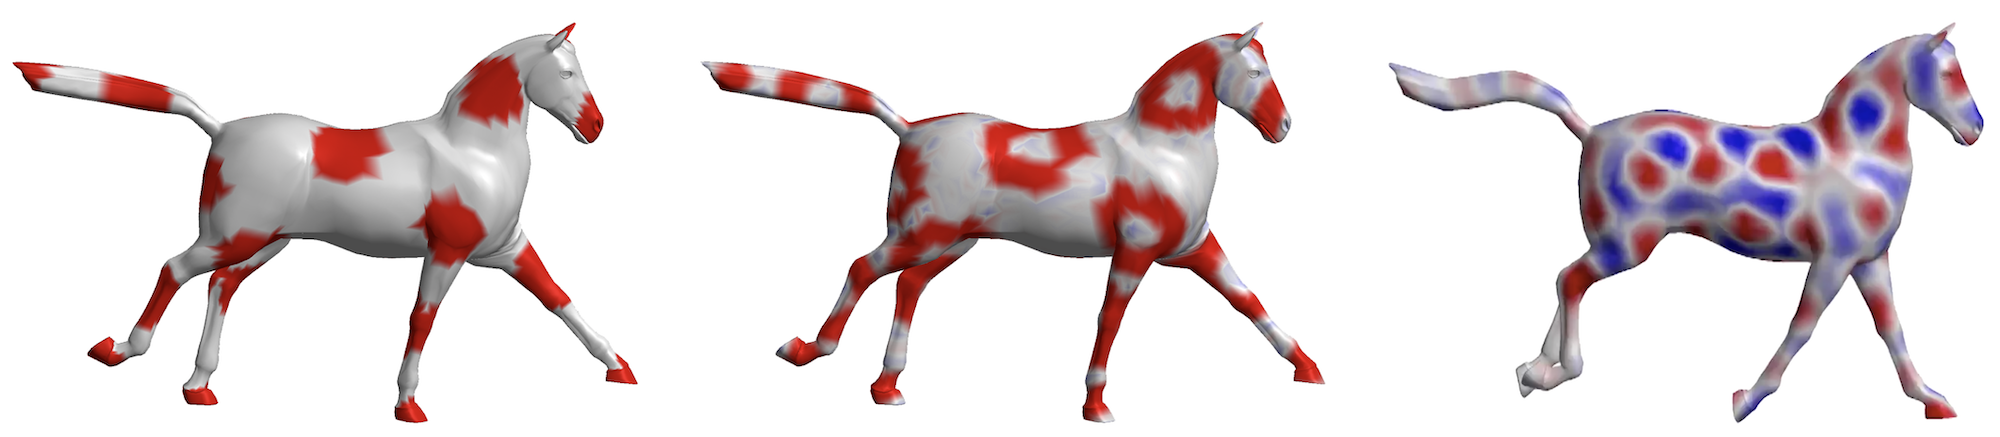
\includegraphics[width=\linewidth]{figures/horses.png}
    \caption{谱滤波器在域扰动下的不稳定性。左：信号 $\mathbf{x}$，位于网格 $\Omega$ 上。中：谱滤波结果%$\mathbf{x}\star \boldsymbol{\theta} = \boldsymbol{\Phi}\, \mathrm{diag}(\hat{\boldsymbol{\theta}}) \boldsymbol{\Phi}^\top \mathbf{x}$
    ，该结果位于%$\boldsymbol{\Phi}$
    Laplacian $\Delta$ 的特征基中，该算子定义在 $\Omega$ 上。
    右：
    同一个谱滤波器 %$\boldsymbol{\theta}$
    作用于%$\bar{\boldsymbol{\Phi}}$
    Laplacian $\tilde{\Delta}$ 的特征向量，该算子属于近似等距扰动域 $\tilde{\Omega}$，
    %(as a result of a near-isometric deformation of the mesh)  
%    $\bar{\boldsymbol{\Phi}}\, \mathrm{diag}(\hat{\boldsymbol{\theta}}) \bar{\boldsymbol{\Phi}}^\top \mathbf{x}$
    产生了截然不同的结果。
    }
    \label{fig:mesh_horses}
\end{figure}%




%
在实践中，由于需要对角化 Laplacian，直接计算~（\ref{eqn:conv_spectral}）的代价高得难以承受。更糟的是，
%, as we will see in Section~\ref{sec:meshes}, 
它在几何上并不稳定：即使域 $\Omega$ 只受到很小的近似等距扰动，Laplacian 的高频特征函数也可能发生显著变化（见图~\ref{fig:mesh_horses}）。
%
%
更稳定的解决方案是把滤波器实现为形如 $\hat{p}(\Delta)$ 的{\em 谱传递函数}：
%which is understood in the operator sense as %\marginnote{Geometric Deep Learning methods based on spectral convolution expressed through the Fourier transform are often referred to as `spectral' and opposed to `spatial' methods we have seen before in the context of graphs. When expressed as spectral transfer function, the former in fact boil down to the latter, so this dichotomy is somewhat artificial and not completely appropriate.}
\begin{eqnarray}
(\hat{p}(\Delta) x)(u) &=& \sum_{k\geq 0} \hat{p}(\lambda_k) \langle x, \varphi_k\rangle \varphi_k (u) \label{eqn:conv_spec} \\
%
&=& \int_\Omega x(v) \, \sum_{k\geq 0} \hat{p}(\lambda_k) \varphi_k(v) \varphi_k (u) \, \mathrm{d}v \label{eqn:conv_spat}
\end{eqnarray}
%
它可以有两种解释：一是解释为谱滤波器~（\ref{eqn:conv_spec}），其中令 $\hat{\theta}_k = \hat{p}(\lambda_k)$；二是解释为空间滤波器~（\ref{eqn:conv_spat}），其位置相关核为 $\theta(u,v) = \sum_{k\geq 0} \hat{p}(\lambda_k) \varphi_k(v) \varphi_k (u)$。
%
%
这种表述的优点是，$\hat{p}(\lambda)$ 可以用少量系数参数化；选择多项式等参数函数\marginnote{基于通过 Fourier 变换表达的谱卷积之几何深度学习方法，常称为“谱”方法，并与此前在图语境下看到的“空间”方法相对。这里可以看出，这两种观点可能等价，因此这种二分有些人为，并不完全恰当。}$\hat{p}(\lambda) = \sum_{l=0}^r \alpha_l \lambda^l$ 后，可以高效地把滤波器计算为
$$
(\hat{p}(\Delta) x)(u) = \sum_{k\geq 0} \sum_{l= 0}^r \alpha_l \lambda_k^l \, \langle x, \varphi_k\rangle \varphi_k (u) = \sum_{l= 0}^r \alpha_l (\Delta^l x)(u),
$$
从而完全避免谱分解。
%
第~\ref{sec:meshes} 节将更详细地讨论这一构造。

%\michael{Add note on stability}

%While filters defined in this manner are isotropic (direction-unaware), 



\paragraph{流形上的空间卷积}

第二种选择是尝试通过在不同点匹配滤波器来定义流形上的卷积，就像式~（\ref{eq:group-conv}）中所做的那样：
%
\begin{equation}
(x \star \theta)(u) = \int_{T_u \Omega} x(\exp_u Y) \theta_u(Y) \mathrm{d}Y, 
\label{eq:conv_tangent_space}
\end{equation}
%
其中，现在必须使用指数映射从切空间访问标量场 $x$ 的值，并且
滤波器 $\theta_u$ 定义在每一点的切空间中，因而依赖于位置。%
如果以内蕴方式定义滤波器，这类卷积就具有等距不变性；前文已指出，这一性质在许多计算机视觉与图形学应用中至关重要。
%, and we use the exponential map to obtain. 


不过，需要注意它与第~\ref{sec:grids_euclidean}--\ref{sec:groups} 节此前构造之间的几个实质区别。
%
第一，由于流形通常不是齐性空间，不再具有允许共享滤波器的全局群结构；所谓共享，是指使用相同的 $\theta$ 于每个 $u$，而不是使用 $\theta_u$ 于式~（\ref{eq:conv_tangent_space}）中。因此，不能在一点定义滤波器后再将其移动到各处。
%as we did in formula~(\ref{eq:group-conv}). 
%
在流形上类比这一运算需要平行输运，使共享滤波器 $\theta$（定义为 $T_u\Omega$ 上的函数）能够应用于另一个 $T_v\Omega$。
%
然而，正如前面所见，这通常取决于 $u$ 与 $v$ 之间的路径，因此{\em 移动滤波器的方式很重要}。%\marginnote{As a possible remedy, \cite{poulenard2018multi} suggested moving the filter along geodesics. }
%
%
第三，由于指数映射只能在局部使用，滤波器必须是{\em 局部的}，其支撑受单射半径限制。
%
第四，
也是最关键的一点，不能直接使用 $\theta(X)$，因为 $X$ 是抽象几何对象；为了用于计算，必须把它{\em 相对于某个局部基}表示出来，
该局部基为 $\omega_u : \mathbb{R}^s \rightarrow T_u\Omega$，所得表示是 $s$ 维坐标数组 $\mathbf{x} = \omega^{-1}_u(X)$。
%
由此可以把卷积~（\ref{eq:conv_tangent_space}）重写为
%
\begin{equation}
(x \star \theta)(u) = \int_{[0,1]^s} x(\exp_u (\omega_u \mathbf{y})) \theta(\mathbf{y}) \mathrm{d}\mathbf{y}, 
\label{eqn:conv_exp}
\end{equation}
%

%\joan{We have used $\delta$ in the previous sections to refer to the size of the filter support}

其中滤波器定义在单位立方体上。由于指数映射是内蕴的（通过测地线定义），所得卷积具有等距不变性。


然而，这里默认假设可以把标架 $\omega_u$ 一同带到另一个流形，即 $\omega_u' = \mathrm{d}\eta_u \circ \omega_u$。
%
%Yet, we should point to one issue that at a close inspection opens a can of worms: in our definition, we assumed $\omega$ was given, which 
不过，仅给定流形 $\Omega$ 时，要以一致方式获得
这样的标架（物理学术语称为\emph{规范}）困难重重。
%implies that we need some mechanism to {\em fix a basis at each point} of the manifold (in physics, a smooth choice of local bases is referred to as a {\em gauge}). 
%
第一，光滑全局规范可能不存在：对于不可\emph{平行化}的流形就是如此。\marginnote{球面 $\mathbb{S}^2$ 是不可平行化流形的一个例子；这一结论源自
%on which one cannot construct a smooth tangent vector field. 
{\em Poincar{\'e}-Hopf 定理}，通俗地说就是“无法在不产生发旋的情况下梳平一个毛球”。\vspace{2mm}
%and is the reason why magnetic plasma confinement chambers must have toroidal rather than spherical geometry. 
%\includegraphics[width=1\linewidth]{figures/hairy_ball.png}
}在这种情况下，无法定义处处非零的光滑切向量场。
%; we further assume that the global gauge is smooth, which is only possible if the manifold is {\em parallelizable}.
%
%
第二，流形上不存在典范规范，因此这种选择具有任意性；由于卷积依赖于 $\omega$，选择不同规范会得到不同结果。

应当指出，这是实践与理论相背离的情形：在实践中，
%one can get around these mathematical issues in a somewhat satisfactory manner.
%That is, 
%there exist algorithms that will 
可以构造大部分区域光滑、仅含有限个奇点的标架，例如取流形上某个内蕴标量场的内蕴梯度。\marginnote{
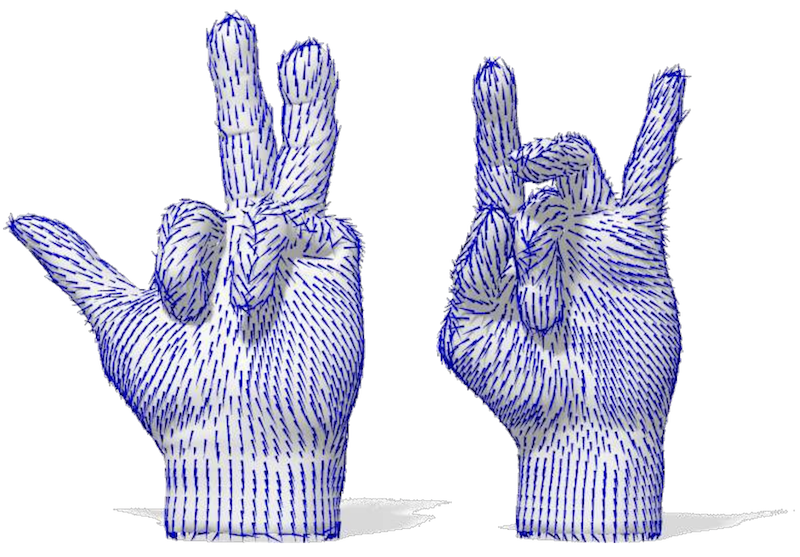
\includegraphics[width=1\linewidth]{figures/gframes.png} 
使用 GFrames 算法 \cite{melzi2019gframes} 在近似等距流形上构造稳定规范的例子（仅显示一个轴）。
} 
%(such as e.g. the North and South pole of the sphere in the sidebar), for instance taking the two frame vectors to correspond to the highest and least curved direction on a 2D manifold. 
%
此外，这类构造具有稳定性，即以这种方式构造的标架在等距流形上相同，在近似等距流形上相似。
%
事实上，早期流形深度学习工作已经采用这类方法 \citep{masci2015geodesic,monti2017geometric}。
%the same frame is found for isometric manifolds, and for nearly isometric ones a similar frame is found. 


不过，这一解决方案并不完全令人满意，因为在奇点附近，滤波器方向（以相对于规范的固定方式定义）会剧烈变化，导致即使输入信号与滤波器光滑，特征图仍不光滑。
%
此外，没有明确理由说明为何点 $u$ 处的某一方向应被视为等价于完全不同点 $v$ 处的另一方向。
%
因此，尽管存在{\em 实用的}替代方案，下面仍将寻找
%methods based on semi-intrinsic frames can be useful, 
一种在{\em 理论上}更有依据、并且完全不依赖规范选择的方法。
%which we will discuss next. 
%We will discuss just such an approach next.


%\joan{This is still a bit long, but already much improved from earlier versions. 
%One aspect that is still not very explicit is how to precisely connect with the GDL blueprint, in terms of the composition of local equivariant maps, and global invariant map. 
%Here we argue that differential operators such as the Laplacian are defined intrinsically (isometry invariant), and thus any representation that is based on it will preserve this isometric invariance. Equivariance in this context is less obvious (equivariance with respect to changes in the gauge, parametrisation/charting?).

%Also, should we mention stability of the Laplacian to metric deformations? How to ensure that the information we extract from the Laplacian is not too unstable? we can mimic the discussion from previous section on wavelet vs fourier, to illustrate that the high-frequency eigenfunctions of the laplace-beltrami  are unstable. THis is mentioned in the mesh section, should it be restated here as well?
%}

%
%
%Assume now we have some vector-valued data $\Omega$. 
%In differential geometry, this is modelled as a {\em vector field} $x:\Omega \rightarrow T\Omega$, assigning to each point $u \in \Omega$ a tangent vector $x(u) \in T_u \Omega$. 
%%
%%
%%The reason we need to consider gauges is that we can only describe geometric data numerically \emph{relative to a gauge}.
%%
%Relative to a gauge, we can express each tangent vector as a coordinate vector, i.e. an array of numbers, and so a vector field becomes a map $\mathbf{x} : \Omega \rightarrow \R^{s}$.
%%
%In other words, we can, as previously, think of vector fields as signals forming the space $\mathcal{X}_{\R^s}(\Omega)$ with the inner product 
%%(\ref{eqn:innerprod}) [Only well defined if we choose a metric? Should we assume Riemannian manifolds?]. 
%$$
%\langle x, y\rangle = 
%\int_\Omega  \langle x(u), y(u) \rangle_{T_u\Omega} du = 
%\int_\Omega \mathbf{x}^\top(u) \mathbf{G}(u) \mathbf{y}(u) du,  
%$$
%%
%where $\mathbf{G}$ is the representation of the {\em Riemannian metric} (defined as an inner product on $T_u\Omega$ depending smoothly on $u$) in the same local frame.
%%

%As in the examples discussed in previous sections, this group can act via different representation $\rho$, which in this case corresponds to different kinds of fields, including scalar fields, vector fields, tensor fields, each of which is characterized by how it transforms under a change of gauge.



%\paragraph{Local Symmetries and Spatial Weight Sharing}


% ----
% OLD:

% Let us start from the simplest case of {\em scalar fields}, i.e. signals $\mathcal{X}(\Omega, \mathbb{R})$. 
% %




% Importantly, not only the {\em features} change when we change the gauge, also the {\em network layers} depend on the choice of gauge. 
% %
% Consider an architecture in the spirit of `message passing' we saw in graph neural networks, where at each point $u\in \Omega$, we aggregate the transformed feature vectors from neighbor points $v$, 
% and 
% %
% for simplicity, assume this transformation is linear. 
% %
% When the vectors are expressed w.r.t. a gauge, this transformation takes the form of matrix multiplication  $\mathbf{A}(u,v)\mathbf{x}(v)$; this notation emphasizes the fact that the matrix can be different for each pair of points $u, v$.  
% %.\marginnote{What we describe here is the GCN architecture. In attentional architectures, we can have $\mathbf{A}(\mathbf{x}(u),\mathbf{x}(u'))$ rather than $\mathbf{A}(u, u')$. }
% %
% %Note however an crucial difference: on a graph, the matrix $\mathbf{A}$ must be {\em the same} for all points $u'$, as this is needed for permutation equivariance. 
% %
% %In the case of a manifold, there is no such a global symmetry, so we can use a different matrix $\mathbf{A}(u,u')$ for each pair of (neighbor) points. 



% If we perform a gauge transformation, the input feature vector changes as $\mathbf{x}(u) \mapsto \rho(\fg(u)) \mathbf{x}(u)$, and the output feature should change as $\mathbf{x}(v) \mapsto \rho(\fg(v)) \mathbf{x}(v)$\marginnote{We assume here for simplicity that the input and output features are of the same type and thus have the same representation $\rho(\fG)$.}.
% It follows that we should change $\mathbf{A}(u,v) \mapsto \rho(\fg(v)) \mathbf{A}(u,v) \rho(\fg(u))^{-1}$.
% Although the new weight matrix and feature vectors contain different numbers, the underlying geometric objects are mapped in the same way regardless of the gauge.



% % Gauge equivariant message; 
% If gauge transformations are considered as symmetries, a network layer, and hence an individual message, should be equivariant to gauge transformations.
% That is, the weight matrix $A_{uu'}$ should satisfy $\rho(g(u'))^{-1} A_{uu'} = A_{uu'} \rho(g(u))$ for all gauge transformations $g : \Omega \rightarrow \fG$.
% This is an extremely strong constraint, because $g(u)$ and $g(u')$ (the gauge transformation at $u$ and $u'$) can vary independently.
% As a consequence the weight matrix $A_{uu'}$ is so constrained that it cannot learn very interesting mappings.

% % Connection
% The solution is to introduce an additional piece of structure called a \emph{connection}, which relates the feature spaces at $u$ and $u'$. % via parallel transport (see Figure TODO).
% The connection gives us for any two nearby points $u, u'$ a straightest curve (geodesic) between them, and a notion of \emph{parallel transport} of frames and feature vectors along this curve (see Figure TODO).
% %The parallel transporter from $u$ to $u'$ along a geodesic is an element of $\fG$ denoted $\fg_{u \rightarrow u'} \in \fG$ that transforms as $\fg_{u \rightarrow u'} \mapsto \fg(u') \fg_{u \rightarrow u'} \fg(u)^{-1}$ under a gauge transformation $\fg(u)$.
% Using parallel transport, we can move the feature vector $v_u$ at $u$ to $u'$, before applying the weight matrix $A_{uu'}$.
% Since this matrix maps input features at $u$ to output features at $u$, it only has to deal with the gauge at $u$.
% In other words, it should satisfy a more conventional equivariance constraint: $A_{uu'} \rho(g(u)) = \rho(g(u)) A_{uu'}$ that only involves $g(u)$ and not $g(u')$. \michael{[TACO: isn't it the other way around, you transport vectors from u' to u?]}

% % Spatial weight sharing; filter on tangent plane; identify tangent planes via gauge;
% What we have seen so far is that gauge symmetries constrain the weight matrix $A_{uu'}$, but that the weight matrices associated with different points need not necessarily share weights as in a convolution layer.




%In each of the examples discussed so far, we started with a space $\Omega$ and a group of symmetries $\fG$ acting on it.
%In some cases however, e.g. when the domain $\Omega$ is a general manifold or mesh, it may not have any obvious symmetries.
%%For instance, if $\Omega$ is a general manifold, it may not have any non-trivial symmetries.
%In this case, we cannot define an action of $\fG$ on the space of signals on $\Omega$ and use it to slide filters around to define a convolution.
%Nevertheless, in this example as many others, there is still a group of symmetries lurking beneath the surface, but this is an altogether kind of symmetry known as \emph{gauge symmetry}.
%
%The word gauge here refers to a choice of frame (ordered basis) for a vector space, or more generally to one such choice for each vector space in a collection of vector spaces $V_u$ associated with the points $u \in \Omega$.
%For example, if we have a manifold $\Omega$, we can construct the \emph{tangent bundle} $T \Omega$ which consists of a collection of vector spaces $T_u \Omega$ (the tangent spaces), one for each point in $u \in \Omega$ (see Figure TODO).
%So in this example a gauge is a choice of frame for each of the tangent spaces $T_u \Omega$.\marginnote{
%We note that in mathematical gauge theory one would require the gauge to be smooth, in which case a globally defined gauge may not always exist. We will ignore these subtleties and not insist on smoothness.
%}
%
%The reason we need to consider gauges is that we can only describe geometric data numerically \emph{relative to a gauge}.
%Let's imagine our data consists of a vector field on $\Omega$.
%A vector field assigns to each point $u \in \Omega$ a tangent vector $v \in T_u \Omega$.
%Relative to a gauge, we can express each tangent vector as a coordinate vector, i.e. a list of numbers, and so a vector field becomes a map $x : \Omega \rightarrow \R^{n}$ (where $n$ is the dimension of the manifold and tangent spaces).
%In other words, our input space is $\mathcal{X}(\Omega, \R^n)$.
%However it is important to realize that what we are really interested in is the underlying geometrical object (vector field), whose representation as a function $x \in \mathcal{X}(\Omega, \R^n)$ depends on the choice of gauge.
%%However there is no canonical choice of gauge, so depending on our choice we will get different coordinate vectors.
%
%When we change the gauge, there is at each position a unique invertible matrix that maps the old gauge to the new one.
%In other words, a gauge transformation is a mapping $g : \Omega \rightarrow \GL{n}$, where $\GL{n}$ is the group of invertible $n \times n$ matrices.
%We can also restrict our attention to e.g. right-handed orthogonal frames, which are related by rotations, in which case a gauge transformation is a map $g : \Omega \rightarrow \SO{n}$ assigning to each position a rotation.
%In general, one considers a group $\fG$ (called the structure group) and a collection of frames such that for any two of them there is a unique $\fg \in \fG$ that maps one frame onto the other.
%As in the examples discussed in previous sections, this group can act via different representation $\rho$, which in this case corresponds to different kinds of fields, including scalar fields, vector fields, tensor fields, each of which is characterized by how it transforms under a change of gauge.
%
%% Associated bundles / reps of G
%% In the previous sections on Graphs, Grids and Groups, we discussed how the same group may act on various feature spaces through different representations $\rho$.
%% In the case of gauge transformations the same is true: we can define various kinds of fields such as scalar, vector, and tensor fields, by choosing an appropriate representation $\rho$ of the structure group $\fG$.
%% For instance, a scalar field (e.g. surface temperature on earth) does not depend on the frame (a scalar does not have a direction), so it corresponds to the trivial representation $\rho_0(g) = 1$.
%% A 2-tensor field would transform as $A_u \mapsto \fg A_u \fg^T$, where $u \in \Omega$, $A_u \in \R^{n \times n}$ and $\fg \in \fG$ is the change of basis matrix relating two gauges.
%
%%Given two vector fields, we can take at each position the outer (tensor) product $v w^T$ to obtain a tensor field, which tra
%
%% Gauge equivariant message from u to v; need for a connection / parallel transport
%%If gauge transformations are considered as symmetries, a network layer should be equivariant to gauge transformations.
%Not only the features change when we change the gauge, also the network layers depend on the choice of gauge.
%We will consider a message passing layer, and focus first on a single message sent from $u \in \Omega$ to $u' \in \Omega$.
%In a graph neural network, one would take the feature vector $v_u$ at $u$ and multiply it by a weight matrix $A$ to get the feature vector $v_{u'}$ at $u'$, before summing over all neighbours $u'$.
%The same weight matrix is used for all pairs of adjacent points $u,u'$, because this is required for equivariance to permutations.
%In the case of a manifold, we don't have such a global symmetry, so we are free to use a different matrix $A_{uu'}$ for each pair of (nearby) points $u, u'$.
%Now if we perform a gauge transformation, the input feature changes as $v_u \mapsto \rho(g(u)) v_u$, and the output feature should change as $v_{u'} \mapsto \rho(g(u')) v_{u'}$\marginnote{We assume here that the input and output feature are of the same type, i.e. have the same representation $\rho$ of $\fG$.}.
%It follows that we should change $A_{uu'} \mapsto \rho(g(u')) A_{uu'} \rho(g(u))^{-1}$.
%Although the new weight matrix and feature vectors contain different numbers, the underlying geometric objects are mapped in the same way regardless of the gauge.
%
%% Gauge symmetries / gauge equivariance
%To say that gauge transformations are symmetries is to say that any two gauges related by a gauge transformation are to be considered equivalent. %, and that data expressed relative to these frames should be processed in the same way regardless of the gauge.
%For instance, if we take $\fG = \SO{n}$, any two right-handed orthogonal frames are considered equivalent, because we can map any such frame to any other such frame.
%In other words, there is are no distinguished local directions such as ``up'' or ``right''.
%Similarly, if $\fG = \Orth{n}$, then any left and right handed orthogonal frame are considered equivalent.
%In this case, there is no preferred orientation either.
%
%% Gauge equivariant message; 
%If gauge transformations are considered as symmetries, a network layer, and hence an individual message, should be equivariant to gauge transformations.
%That is, the weight matrix $A_{uu'}$ should satisfy $\rho(g(u'))^{-1} A_{uu'} = A_{uu'} \rho(g(u))$ for all gauge transformations $g : \Omega \rightarrow \fG$.
%This is an extremely strong constraint, because $g(u)$ and $g(u')$ (the gauge transformation at $u$ and $u'$) can vary independently.
%As a consequence the weight matrix $A_{uu'}$ is so constrained that it cannot learn very interesting mappings.
%
%% Connection
%The solution is to introduce an additional piece of structure called a \emph{connection}, which relates the feature spaces at $u$ and $u'$. % via parallel transport (see Figure TODO).
%The connection gives us for any two nearby points $u, u'$ a straightest curve (geodesic) between them, and a notion of \emph{parallel transport} of frames and feature vectors along this curve (see Figure TODO).
%%The parallel transporter from $u$ to $u'$ along a geodesic is an element of $\fG$ denoted $\fg_{u \rightarrow u'} \in \fG$ that transforms as $\fg_{u \rightarrow u'} \mapsto \fg(u') \fg_{u \rightarrow u'} \fg(u)^{-1}$ under a gauge transformation $\fg(u)$.
%Using parallel transport, we can move the feature vector $v_u$ at $u$ to $u'$, before applying the weight matrix $A_{uu'}$.
%Since this matrix maps input features at $u$ to output features at $u$, it only has to deal with the gauge at $u$.
%In other words, it should satisfy a more conventional equivariance constraint: $A_{uu'} \rho(g(u)) = \rho(g(u)) A_{uu'}$ that only involves $g(u)$ and not $g(u')$.
%
%% Spatial weight sharing; filter on tangent plane; identify tangent planes via gauge;
%What we have seen so far is that gauge symmetries constrain the weight matrix $A_{uu'}$, but that the weight matrices associated with different points need not necessarily share weights as in a convolution layer.
%
%----
%
%% Spatial weight sharing; filter on tangent plane; identify tangent planes via gauge;
%What we have seen so far is that gauge symmetries constrain the weight matrix $A_{uu'}$, but that the weight matrices associated with different points need not necessarily share weights as in a convolution layer.
%In order to share weights across spatial locations, we need to somehow identify local patches around each point in $\Omega$.
%A popular approach is based on the observation that these local patches can first be identified with the tangent planes $T_u \Omega$ via the exponential map (see Figure TODO). %, so that we can write $A_{uu'}$ instead as $A_{uv}$ where $v \in T_u \Omega$ is a tangent vector that satisfies $u' = \exp_u(v)$.
%Furthermore, the tangent spaces themselves can be identified with $\R^n$ through the choice of a gauge.
%Hence, we can define the filter as a matrix-valued function $A$ on $\R^n$ (which parameterizes the neighbour $u'$) and which is independent of $u$.
%
%Since the filter is now tied to the gauge, it will be rotated when we rotate the gauge.
%Hence, the equivariance constraint becomes $A(g v) = \rho(g) A(v) \rho(g)^{-1}$.
%
%Thus, we can define a gauge equivariant convolution of a field $x$ on $\Omega$ and a filter $A$ as follows:
%\begin{equation}
%    (x \star A)(u) = \int_{\R^n} A(v) \, \rho(\fg_{\exp_u(v) \rightarrow u}) \, x(\exp_u(v)) dv,
%\end{equation}
%where $\exp_u(v)$ denotes the neighbour $u'$ indexed by $v \in \R$ and $\fg_{\exp_u(v) \rightarrow u} \in \fG$ denotes the parallel transport from this neighbour to $u$.
%



%---


% If gauge transformations are considered as symmetries, a mapping (network layer) $f : \mathcal{X}(\Omega, \R^n) \rightarrow \mathcal{X}(\Omega, \R^m)$ should be equivariant to gauge transformations.
% As a first example, consider a $1 \times 1$ convolution, i.e. $f$ consists of applying a linear map $\psi : \R^n \rightarrow \R^m$ at each position $u \in \Omega$.
% The input feature vector $v_u \in \R^n$ is a coordinate vector defined relative to some choice of gauge, and we will want that the output feature vector $w_u = \psi(v_u)$ is expressed relative to the same gauge.
% If we change the gauge by $g_u \in \fG$, then the input transforms as $v_u \mapsto \rho_{\textup{in}}(g_u) v_u$ and the output should transform by $w_u \mapsto \rho_{\textup{out}}(g_u) w_u$.
% Hence we $\psi$ should be equivariant: $\psi \circ \rho_{\textup{in}}(g_u) = \rho_{\textup{out}}(g_u) \circ \psi$ for all $g_u \in \fG$.

% The example of a $1 \times 1$ convolution is simple, because the input and output feature vectors $v_u$ and $w_u$ have the same spatial position $u \in \Omega$, and hence are represented with respect to the same gauge.
% In a general convolution, one would sum/integrate the messages sent from points $u'$ near $u$ as well, using a learned map $\psi_{uu'} : \R^n \rightarrow \R^m$.
% For this function we would have the constraint $\psi_{uu'} \circ \rho_{\textup{in}}(g_{u'}) = \rho_{\out}(g_u) \circ \psi_{uu'}$.
% However, since $g_u$ and $g_{u'}$ can vary independently (we can freely change the gauge at each position separately), this is an overly constraint and any $\psi_{uu'}$ that satisfies it will be uninteresting.

% The remedy is to introduce an object called a \emph{connection} that tells us how to compare feature vectors at $u$ and feature vectors at $u'$.
% That is, we take a map $c_{u \rightarrow u'} : \R^n \rightarrow \R^n$ 
% [TBC...]

%[Discuss internal symmetries.]

% In the context of geometric deep learning, the vector space in question is $\mathcal{C}$, i.e. the feature vector space that is attached to each position in $\Omega$ to build the space $\mathcal{X}(\Omega, \mathcal{C})$ of signals $x : \Omega \rightarrow \mathcal{C}$.


% The word gauge here refers to a choice of frame (ordered basis) for a vector space.
% In the context of geometric deep learning, the vector space in question is $\mathcal{C}$, i.e. the feature vector space that is attached to each position in $\Omega$ to build the space $\mathcal{X}(\Omega, \mathcal{C})$ of signals $x : \Omega \rightarrow \mathcal{C}$.
% Consider for now just a single copy of $\mathcal{C}$.
% We know from linear algebra that a linear map $f : \mathcal{C} \rightarrow \mathcal{C}$ can be expressed as a matrix $A$ if we choose a frame for $\mathcal{C}$, and likewise a vector $V \in \mathcal{C}$ can be represented as a coordinate vector $v \in \R^n$.
% If we change the frame, the matrix representation of $f$ changes as $A \mapsto P A P^{-1}$, where $P$ is called the change of basis matrix in linear algebra, or gauge transformation, in physics.
% The coordinate vector changes as $v \mapsto P v$.

% If we consider $P$ as a gauge \emph{symmetry}, then $A$ should be equivariant, i.e. $PA = AP$.
% Equivalently, we should have $A = PAP^{-1}$, i.e. $A$ has the same matrix representation in all frames related by a gauge symmetry.
% Hence, the matrix $A$ can be applied to coordinate vectors not just in one frame, but also to any other frame related by a gauge symmetry.
% For instance, if we consider the group of rotations as gauge symmetries, then any two orthogonal frames of the same handedness can be considered equivalent and $A$ can be applied to coordinate vectors in any such frame.
% Similarly, if we consider both rotations and reflections to be gauge symmetries, the same is true for orthogonal frames of different handedness.

% In gauge theory, this idea is generalized in two ways.
% Firstly, since we are dealing with signals $x : \Omega \rightarrow \mathcal{C}$, we have not just one vector space $\mathcal{C}$, but one copy of $\mathcal{C}$ associated with every point $u \in \Omega$.\marginnote{The vector space attached at $u \in \Omega$ is sometimes called the fibre $\mathcal{C}_u$ at $u$.}
% We are free to choose a different basis for each of these vector spaces, and so a general gauge transformation consists of one transformation at each point in $\Omega$.
% In other words, a gauge transformation is a function $g : \Omega \rightarrow \fG$, where $\fG$ is called the structure group (e.g. rotations or roto-reflections in the examples above).

% Secondly, as in the case of global symmetries acting on $\Omega$, one may consider different representations $\rho$ of the same group $\fG$ in each feature space in the network.
% Thus, if we have a representation $\rho$ of $\fG$ in $\mathcal{C}$, then a gauge transformation $g : \Omega \rightarrow \fG$ acts on a signal $x : \Omega \rightarrow \mathcal{C}$ as $x(u) \mapsto \rho(g(u)) x(u)$.  % todo check if we need an inverse on g?

% \taco{TODO: work on formatting of examples}
% \begin{tcolorbox}[width=\linewidth,
%                   boxsep=0pt,
%                   left=7.5pt,
%                   right=7.5pt,
%                   top=7.5pt,
%                   bottom=7.5pt,
%                   arc=0pt,
%                   boxrule=0pt,toprule=0pt,
%                   colback=boxgray,
%                   ]%%
%     Example: tangent vectors on a manifold.
    
%     Consider a smooth manifold $\Omega$ of dimension $2$.
%     % For instance, $\Omega$ could be an iso-energy surface of a protein [cite Michael's paper].
%     At each point $u \in \Omega$, there is a tangent space $T_u \Omega$ (see Figure TODO).
%     A \emph{vector field} is an assignment of a vector $v_u \in T_u \Omega$ to each point $u \in \Omega$.
%     If we choose a frame for each tangent space, we can express a vector field as a function $v : \Omega \rightarrow \R^2$.
%     ...
% \end{tcolorbox}


% \begin{tcolorbox}[width=\linewidth,
%                   boxsep=0pt,
%                   left=7.5pt,
%                   right=7.5pt,
%                   top=7.5pt,
%                   bottom=7.5pt,
%                   arc=0pt,
%                   boxrule=0pt,toprule=0pt,
%                   colback=boxgray,
%                   ]%%
%     Example: color space symmetry.
    
    
% \end{tcolorbox}


%Typically a problem comes with a fixed structure group $\fG$ and space $\Omega$, but the feature spaces $\mathcal{X}(\Omega, \mathcal{C}_l)$ at each layer $l$ may 

% the matrix $A$ can be applied to coordinate vectors in any equivalent basis; if $w = Av$ and we change the basis, $v' = P v$ then $w' = A P v = P A v = P w$.
% That is, if we apply $A$ to a coordinate vector relative some basis, we get an output coordinate vector relative to the same basis.



% To postulate a gauge symmetry is to postulate that frames related by certain kinds of gauge transformations are equivalent.
% For instance, two frames related by a rotation or reflection, can be considered equivalent.
% Or if we care about handedness, only those frames related by a rotation should be considered equivalent.



% Both global symmetries acting on $\Omega$ and gauge symmetries acting on $\mathcal{C}$ change how a signal is represented numerically, e.g. in computer memory.
% However, whereas global symmetries considered act on the domain $\Omega$, gauge symmetries act on the range $\mathcal{C}$ of signals $x : \Omega \rightarrow \mathcal{C}$.
% For example, in the case of graphs, a permutation will shuffle the node feature vectors but not change the feature vectors themselves.
% Conversely, a gauge transformation will change the feature vectors but not move them around on $\Omega$.


\subsection{规范与丛}
\label{sec:gauges}

我们已把规范定义为切空间的标架；不过，规范概念
%In the previous section we have already touched on the concept %of a gauge, defining it as a frame for the tangent space. 
%
%The notion of gauge as used in physics is however 
在物理学中一般得多：它可以指任意\marginnote{从历史上看，纤维丛最早出现在 {\'E}lie Cartan 的现代微分几何中（但他没有显式定义它们），随后在 20 世纪 30 年代的拓扑学中被进一步发展为独立对象。}\emph{向量丛}的标架，而不仅是切丛的标架。
%
非形式地说，向量丛描述由另一个空间参数化的一族向量空间，并且
由\emph{底空间} $\Omega$ 构成；底空间中每个位置都附着同一个向量空间 $\mathbb{V}$（称为\emph{纤维}），该位置为 $u \in \Omega$（对于切丛，纤维就是切空间 $T_u\Omega$）。
%and a continuous {\em projection function} $\pi : V \rightarrow \Omega$. 
%
粗略地说，丛在局部看起来像乘积 $\Omega \times \mathbb{V}$，这里所说的局部是点 $u$ 周围；但在全局上，丛可能发生“扭曲”，从而具有不同的整体结构。
%
%A {\em section} of the bundle is a 
%collection of identical vector spaces attached to the points in the manifold $\Omega$. 
%
%
%
%
在几何深度学习中，纤维%in question are
可用于对流形 $\Omega$ 中每一点的特征空间建模，纤维维数等于特征通道数。
在这一语境下，可能会出现一种新颖而迷人的对称性，称为\emph{规范对称性}。% \joan{Good opening. Can we give a concrete example of this symmetry? Physics application?}

%[Say something about setting? Assume manifold is known and the same for all data points. Each data point is a different signal on it. This is different from previous section where we assume manifold is different for each data point / manifold is part of the data.]


%\joan{Mobius strip}

%\joan{Field theory invariants -- ask Kyle for a nice example}
%Before we discuss the general case, 


再次考虑 $s$ 维流形 $\Omega$ 及其切丛 $T\Omega$，以及向量场
%consider again a vector field 
$X : \Omega \rightarrow T \Omega$（在这一术语中称为切丛上的一个{\em 截面}）。
%
相对于切丛的规范 $\omega$，$X$ 表示为函数 $\mathbf{x} : \Omega \rightarrow \R^s$。
不过，重要的是认识到我们真正关心的是底层几何对象（向量场）；它作为函数 $\mathbf{x} \in \mathcal{X}(\Omega,\R^s)$ 的表示{\em 依赖于规范的选择} $\omega$。
%
如果改变规范，也需要改变 $\mathbf{x}$，以保持其所表示的底层向量场不变。

%\michael{Give a comment from physics where this need arises: general relativity?}

%Likewise, we then need to change the layers of the network so that when they receive inputs expressed relative to the new gauge, they also produce outputs relative to that gauge; like a change of basis, but for many vector spaces at once.

% Taco: note, this itself is not gauge equivariance yet. Only if we *dont* need to change the map, yet it passes through gauge transformations, we have gauge equivariance.
%Since there is no `canonical' way to set a gauge, 
%we must ensure $x$ transforms appropriately when the gauge is changed -- a property we will call {\em gauge-equivariance}. 

%
%\begin{figure}[h!]
%    \centering
%    %\includegraphics{}
%    \caption{TODO: figure showing a manifold with a vector field on it, with one tangent plane drawn. In this tangent plane, a frame is drawn. The coordinates of the vector on that tangent plane is shown below. On the right, an identical figure but with a different frame, and different coordinates. Alternatively, we can draw a plane with a vector field on it. Then we dont draw tangent planes but we draw frames at regularly spaced intervals. The vector field is the same for the left and right figure, but the frame is different.}
%    \label{fig:into:vector-field-gauge}
%\end{figure}


%However there is no canonical choice of gauge, so depending on our choice we will get different coordinate vectors.

%\joan{Here we could already give a couple of examples. 
%
%}


\paragraph{切丛与结构群}
改变规范时，需要在每一点应用一个把旧规范映射到新规范的可逆矩阵。对每一点处的每一对规范，该矩阵都是唯一的，但在不同点处可能不同。
%
%\marginnote{We can also restrict our attention to e.g. right-handed orthogonal frames, which are related by rotations, in which case a gauge transformation is a map $\fg : \Omega \rightarrow \SO{s}$ assigning to each position a rotation.} 
换言之，{\em 规范变换}是映射 $\fg : \Omega \rightarrow \GL{s}$，其中 $\GL{s}$ 是由可逆 $s \times s$ 矩阵组成的{\em 一般线性群}。
它作用于规范 $\omega_u : \R^s \rightarrow T_u \Omega$，产生新规范 $\omega'_u = \omega_u \circ \fg_u : \R^s \rightarrow T_u \Omega$。
%
规范变换作用于坐标向量场%$\mathbf{x}$
的每一点，
通过 $\mathbf{x}'(u) = \fg^{-1}_u \mathbf{x}(u)$ 产生坐标表示 $\mathbf{x}'$，它相对于新规范表示 $X$。
%
底层向量场保持不变：
$$
X(u) = \omega'_u(\mathbf{x'}(u)) = \omega_u( \fg_u \fg^{-1}_u \mathbf{x}(u)) = \omega_u(\mathbf{x}(u)) = X(u), 
$$
这正是所期望的性质。
%
%
%
更一般地，可以考虑按照表示 $\rho$ 变换的几何量场，而该表示属于 $\GL{s}$；例如二阶张量（矩阵）场 $\mathbf{A}(u) \in \R^{s \times s}$，其变换方式为 $\mathbf{A'}(u) = \rho_2(\fg^{-1}_u) \mathbf{A}(u) = \rho_1(\fg_u) \mathbf{A}(u) \rho_1(\fg^{-1}_u)$。%\michael{The notation here is confusing: before we had $\rho$ as a matrix acting on vectors. Here it acts on both sides of $A$. Perhaps we should already mention the same thing when talking about graphs, where we have the representation of permutations acting on the adjacency matrix? }
%\taco{Decision: use $\mathbf{R}$ as the matrix representation of $\fg$}
在这种情形下，规范变换 $\fg_u$ 通过 $\rho(\fg_u)$ 作用。

有时可能只关注具有某种性质的标架，例如正交标架、右手标架等。
自然地，我们关心的是一组保持某种性质并构成群的变换。
例如，保持正交性的群是正交群 $\Orth{s}$（旋转与反射），而还保持定向或“手性”的群是 $\SO{s}$（纯旋转）。
因此，一般而言有一个称为丛之\emph{结构群}的群 $\fG$，规范变换则是映射 $\fg : \Omega \rightarrow \fG$。
关键观察是：在所有具有给定性质的情形下，对于给定点处的任意两个标架，恰有一个规范变换将它们联系起来。

%\taco{Introduce parallel transport here? Say it is $\fG$-valued}

如前所述，规范理论不局限于切丛；一般而言，可以考虑向量空间丛，其结构和维数未必与底空间 $\Omega$ 的结构和维数相关。\marginnote{我们用 $s$ 表示底空间 $\Omega$ 的维数，用 $d$ 表示纤维维数。对于切丛，$d=s$ 是底层流形的维数。对于 RGB 图像，$s=2$ 且 $d=3$。}
例如，彩色图像像素在二维网格上的位置为 $u \in \Omega = \Z^2$，在 RGB 空间中的取值为 $\mathbf{x}(u) \in \R^3$；因此，可以把像素空间视为一个向量丛，其底空间为 $\Z^2$，每一点附着纤维 $\R^3$。
%
通常相对于这样一种规范来表示 RGB 图像：该规范依次以 R、G、B 为基向量，因此图像的坐标表示为 $\mathbf{x}(u) = (r(u), g(u), b(u))^\top$。
也可以在每个位置独立置换基向量（颜色通道），只要记住每一点采用的标架（通道顺序）即可。\marginnote{在本例中，我们选择 $\fG = \Sigma_3$，即三个颜色通道的置换，作为丛的结构群。也可以采用其他选择，例如色相旋转 $\fG = \SO{2}$。}
作为计算操作，这样做并没有多少意义；但正如稍后将看到的，从概念上考虑 RGB 颜色空间的规范变换很有用，因为它允许表达规范对称性——在本例中即颜色之间的等价性——并使定义在图像上的函数遵守这一对称性（等同地对待每种颜色）。




与流形上的向量场情形类似，RGB 规范变换会改变图像的数值表示（在每个像素处独立置换 RGB 值），但不会改变底层图像。
%
在机器学习应用中，我们关心构造这类图像上的函数 $f \in \mathcal{F}(\mathcal{X}(\Omega))$（例如执行图像分类或分割），并将其实现为神经网络层。
%
因此，如果出于某种原因对图像施加规范变换，也需要相应改变函数 $f$（网络层），以保持其含义。
为简单起见，考虑 $1 \times 1$ 卷积，即把 RGB 像素 $\mathbf{x}(u) \in \R^3$ 映射为特征向量 $\mathbf{y}(u) \in \R^C$ 的映射。
按照几何深度学习蓝图，输出与群表示 $\rho_{\textup{out}}$ 相关联；在本例中，这是 $C$ 维表示，属于结构群 $\fG = \Sigma_3$（RGB 通道置换）。类似地，输入与表示 $\rho_{\textup{in}}(\fg) = \fg$ 相关联。%\michael{not clear: is $\fg$ a permutation here? You need to define how the C-dim representation of the permutation looks like}
随后，若对输入施加规范变换，就需要把线性映射（$1 \times 1$ 卷积）$f : \R^3 \rightarrow \R^C$ 改为 $f' = \rho^{-1}_{\textup{out}}(\fg) \circ f \circ \rho_{\textup{in}}(\fg)$，使输出特征向量 $\mathbf{y}(u) = f(\mathbf{x}(u))$ 在每一点都按 $\mathbf{y}'(u) = \rho_{\textup{out}}(\fg_u) \mathbf{y}(u)$ 变换。
确实可以验证：
\begin{equation*}
    \mathbf{y}' = f'(\mathbf{x}') = \rho^{-1}_{\textup{out}}(\fg) f(\rho_{\textup{in}}(\fg) \rho^{-1}_{\textup{in}}(\fg) \mathbf{x}) = \rho^{-1}_{\textup{out}}(\fg) f(\mathbf{x}).\marginnote{Here the notation $\rho^{-1}(\fg)$ should be understood as the inverse of the group representation (matrix) $\rho(\fg)$.}
\end{equation*}

%\joan{Indeed, here I would illustrate these formulas in terms of their matrix representations. If $P_{\fg}$ is a $3x3$ permutation matrix and $F$ the linear (trainable) map expressed as a $C \times 3$ matrix, then we wish to characterise the matrices $Q_{\fg}$ indexed by the group $\Sigma_3$ so that
%$Q_{\fg}^{-1} F P_{\fg} $ does not depend on $\fg$, and thus 
%$Q_{\fg}^{-1} F P_{\fg} = F$ for all $\fg$?
%is this the main idea? }

%\michael{show an example! too abstract}

% Gauge symmetries / gauge equivariance
\paragraph{规范对称性}
把规范变换视为对称性，意味着由规范变换联系起来的任意两个规范都应视为等价。%, and that data expressed relative to these frames should be processed in the same way regardless of the gauge.
例如，若取 $\fG = \SO{d}$，则任意两个右手正交标架都被视为等价，因为可以通过旋转将其中任意一个标架映射为另一个。
换言之，不存在“上”或“右”这类特殊的局部方向。
同样，若 $\fG = \Orth{d}$（正交群），则任意左手或右手正交标架都被视为等价。
在这种情况下，也不存在优先选定的定向。
%
%
%
一般而言，可以考虑一个群 $\fG$ %  \marginnote{Such $\fG$ is called the {\em structure group} of the (tangent) bundle.}
以及每个点 $u$ 处的一组标架，使得其中任意两个标架之间都存在唯一的 $\fg(u) \in \fG$，将一个标架映射为另一个。
%

%\joan{Beware notation; is $d$ the right choice here?}

在几何深度学习蓝图中把规范变换视为对称性时，我们关注的是使
%network layers 
函数 $f$ 作用于定义在 $\Omega$ 上并相对于规范表示的信号，并且对于这种变换具有等变性。
%
具体而言，这意味着如果对输入施加规范变换，输出也应经历同样的变换（但可能通过 $\fG$ 的另一种表示起作用）。
前面已经指出，改变规范时函数 $f$ 也应随之改变；但对规范等变映射而言并非如此：改变规范并不会改变该映射。
为说明这一点，再来看 RGB 颜色空间的例子。
若 $f : \R^3 \rightarrow \R^C$ 满足 $f \circ \rho_{\textup{in}}(\fg) = \rho_{\textup{out}}(\fg) \circ f$，则该映射是等变的；而此时施加于 $f$ 的规范变换没有作用：$\rho_{\textup{out}}^{-1}(\fg) \circ f \circ \rho_{\textup{in}}(\fg) = f$。
换言之，规范等变映射的坐标表达式与规范无关，这与图上的情形类似：
无论输入节点如何置换，我们都应用同一个函数。
%a graph neural network applies the same layers 
%
不过，与图以及此前讨论的其他例子不同，规范变换{\em 并不作用于} $\Omega$，而是分别作用于{\em 每一个特征向量} $\mathbf{x}(u)$；所用变换为 $\fg(u) \in \fG$，其中每个 $u \in \Omega$ 都有各自的变换。
%\joan{This paragraph is not very easy to understand. Have we defined a `Gauge equivariant map' before? I think indeed it is a good idea to relate this notion to the previously introduced equivariances in graphs and grids.  }
%\taco{This paragraph is my attempt at defining them informally (see ``concretely ...'').}

%Different signals defined on $\Omega$ (e.g. scalar fields, vector fields, tensor fields) are affected differently by the action of $\fG$, which acts on them through the corresponding representation $\rho$ of $\fG$.
%

当考察流形上具有更大空间支撑的滤波器时，还需要考虑更多因素。
%
先考虑一个简单例子：%: a network layer that maps
映射 $f : \mathcal{X}(\Omega, \mathbb{R}) \rightarrow \mathcal{X}(\Omega, \mathbb{R})$ 将
$s$ 维流形 $\Omega$ 上的标量场映射为标量场。
与向量及其他几何量不同，标量没有方向，因此标量场 $x \in \mathcal{X}(\Omega, \R)$ 对规范变换是{\em 不变的}（它按照平凡表示 $\rho(\fg) = 1$ 变换）。
%\joan{assuming unitary gauges I guess?}. \taco{If we define scalar as ``transforming according to the trivial rep'' then no: we can have GL structure group / general frames, and yet have invariant scalars. E.g. one might have a 2D tangent plane with general linear frames, but a function on $\Omega$ doesn't care if you rotate or scale the frame. On the other hand one could define a 1D geometric quantity that transforms by the determinant of the gauge transformation (det being a non-unitary 1D rep.) But I think this is not whats usually meant by scalar in physics.}
因此，从标量场到标量场的任意线性映射都是{\em 规范等变的}（在这种情况下也就是不变的）。
例如，可以仿照~（\ref{eqn:conv_spat}）写出 $f$，把它表示为使用位置相关滤波器 $\theta : \Omega \times \Omega \rightarrow \R$ 的卷积型运算，%\michael{defined this way it's not local. Nor that in the Euclidean filter the filter is required to be local - a circulant matrix can be full, this is just a design consideration. }
\begin{equation}
    \label{eq:intro:general-linear-map-scalar-fields}
    (x \star \theta)(u) = \int_{\Omega} \theta(u, v) x(v) \mathrm{d}v.  
\end{equation}
这意味着每个点都可能具有不同的滤波器 $\theta_u = \theta(u, \cdot)$，即不存在空间权重共享——而仅凭规范对称性并不能提供这种共享。
%require spatial weight sharing, for it acts separately on each point in $\Omega$.


现在考虑一个更有意思的情形：映射 $f : \mathcal{X}(\Omega, T\Omega) \rightarrow \mathcal{X}(\Omega, T\Omega)$ 将向量场映射为向量场。
%
相对于某个规范，输入与输出向量场 $X, Y \in \mathcal{X}(\Omega, T\Omega)$ 是向量值函数 $\mathbf{x}, \mathbf{y} \in \mathcal{X}(\Omega, \R^s)$。
%
这类函数之间的一般线性映射可以用此前标量情形的同一个式子（\ref{eq:intro:general-linear-map-scalar-fields}）写出，只需把标量核替换为矩阵值核 $\boldsymbol{\Theta} : \Omega \times \Omega \rightarrow \R^{s \times s}$。
%
矩阵 $\boldsymbol{\Theta} (u, v)$ 应把 $T_v\Omega$ 中的切向量映射到 $T_u\Omega$ 中的切向量，但这两个点具有{\em 不同的规范}，而且我们可以{\em 任意且独立地}改变它们。
%
 也就是说，滤波器必须满足 $\boldsymbol{\Theta} (u, v) = \rho^{-1}(\fg(u)) \boldsymbol{\Theta}(u, v) \rho(\fg(v))$，而且这一关系对所有 $u, v \in \Omega$ 都成立；其中 $\rho$ 表示 $\fG$ 在向量上的作用，由一个 $s\times s$ 旋转矩阵给出。
 %
由于 $\fg(u)$ 和 $\fg(v)$ 可以自由选择，这对滤波器施加了过强的约束。\marginnote{事实上，在这种情况下 $\boldsymbol{\Theta}$ 必须为零。}
%\michael{Perhaps explain why: give a 2D example?}


更好的方法是先利用联络把向量移动到同一个切空间，再只针对某一点处的单个规范变换施加规范等变性。
%To obtain a non-trivial mapping between vector fields, we require a connection which allows us to parallel transport vectors between two tangent spaces. 
于是，可以不用式（\ref{eq:intro:general-linear-map-scalar-fields}），而定义如下向量场之间的映射：
\begin{equation}
    (\mathbf{x} \star \boldsymbol{\Theta})(u) = \int_\Omega \boldsymbol{\Theta}(u, v) \rho(\fg_{v \rightarrow u}) \mathbf{x}(v) \mathrm{d}v,\label{eqn:gauge_eq_conv}
\end{equation}
其中，$\fg_{v \rightarrow u} \in \fG$ 表示沿连接这两个点的测地线从 $v$ 到 $u$ 的平行输运；
%
其表示 $\rho(\fg_{v \rightarrow u})$ 是一个 $s \times s$ 旋转矩阵，在向量于两点之间移动时对其进行旋转。
%
请注意，这里假定该测地线是唯一的；这一点只在局部成立，因此滤波器必须具有局部支撑。
%
%
在规范变换 $\fg_u$ 下，该元素按照 $\fg_{u \rightarrow v} \mapsto \fg_u^{-1} \fg_{u \rightarrow v} \fg_v$ 变换，而场本身按照 $\mathbf{x}(v) \mapsto \rho(\fg_v) \mathbf{x}(v)$ 变换。
如果滤波器与结构群表示可交换，即 $\boldsymbol{\Theta}(u, v) \rho(\fg_u) = \rho(\fg_u) \boldsymbol{\Theta}(u, v)$，%the above map is gauge-equivariant.
则式~（\ref{eqn:gauge_eq_conv}）定义了一个{\em 规范等变卷积}，它按照下式变换：
$$ 
(\mathbf{x}' \star \boldsymbol{\Theta})(u) = \rho^{-1}(\fg_u) (\mathbf{x} \star \boldsymbol{\Theta})(u). 
$$ 
这里采用的正是上述变换。%substitutions, we find that

%, where $\mathbf{x}(u) = \rho(\fg_u)^{-1} \mathbf{x}$.
% \begin{equation}
%     \int_\Omega \psi(u, v) \rho(\fg_u^{-1} \fg_{v \rightarrow u} \fg_v) \rho(\fg_v) \mathbf{x}(v) dv
%     = 
%     \rho(\fg_u)^{-1} \int_\Omega \psi(u, v) \rho(\fg_{v \rightarrow u}) \mathbf{x}(v) dv
% \end{equation}


% [Mention spatial weight sharing: covered in models section. Maybe explain basic idea in words here.]

%\taco{TODO: say that rho of PT is a rotation matrix. +Figure?}



\subsection{几何图与网格曲面}
\label{sec:meshes}

最后，我们以{\em 几何图}（即能够在某个几何空间中实现的图）和{\em 网格曲面}结束对不同几何域的讨论。
%
%
在几何域的“5G”中，网格曲面介于图与流形之间：它们在许多方面与图相似，但其附加结构又使我们能够以类似连续对象的方式处理它们。
%
因此，我们在这一框架中并不把网格曲面视为独立对象；事实上，我们将强调，本节针对网格曲面推导的许多构造也可直接用于一般图。
%




正如第~\ref{sec:manifolds} 节已经提到的，二维流形（曲面）是建模 3D 对象（更准确地说，是这些对象的边界曲面）的常用方式。在计算机图形学和视觉应用中，这类曲面通常被离散化为{\em 三角网格曲面}，\marginnote{三角网格曲面是称为{\em 单纯复形}的一类拓扑结构的实例。}
可以粗略地把它看作沿边粘合三角形而得到的曲面分片平面近似。
%
因此，网格曲面是（无向的）{\em 带附加结构的图}：除了节点和边之外，网格曲面
$\mathcal{T} = (\mathcal{V},\mathcal{E}, \mathcal{F})$ 
还具有构成{\em 三角形面}的有序节点三元组 $\mathcal{F} =  \{ (u,v,q) : u,v,q \in \mathcal{V} \,\,\, \text{and} \,\,\, (u,v), (u,q), (q,v) \in  \mathcal{E}\}$；节点的顺序定义了面的{\em 定向}。\marginnote{
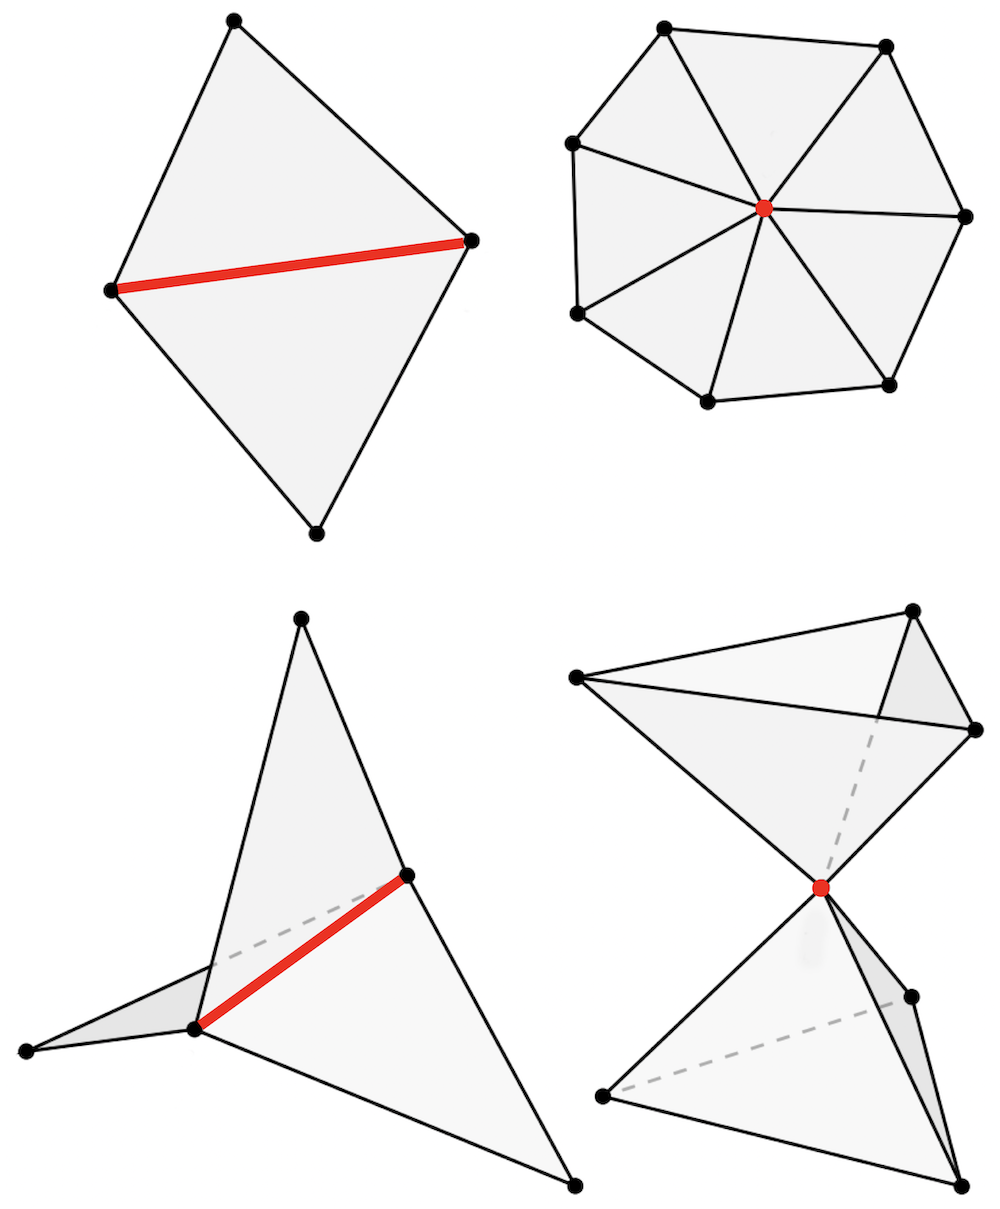
\includegraphics[width=0.9\linewidth]{figures/mesh.png}\\
%
流形边和节点（上）与非流形边和节点（下）的示例。
对于带边界流形，还要定义只属于一个三角形的{\em 边界边}。}
%
%We will denote meshes by $\mathcal{T} = (\mathcal{V},\mathcal{E}, \mathcal{F})$, where $\mathcal{F} =  \{ (i,j,k) : i,j,k \in \mathcal{V} \,\,\, \text{and} \,\,\, (i,j), (i,k), (k,j) \in  \mathcal{E}\}$ and use them as our domain $\Omega$.  


还要进一步假定，每条边恰好由两个三角形共享，并且与每个节点关联的所有三角形之边界构成单一的边环。这一条件保证每个节点周围的一跳邻域都呈圆盘状，从而使网格曲面构成{\em 离散流形}——这样的网格曲面称为{\em 流形网格曲面}。
%In particular, 
%
%
%
与 Riemann 流形类似，可以在网格曲面上定义{\em 度量}。在最简单的情形下，它可以由网格节点 $\mathbf{x}_1, \hdots, \mathbf{x}_n$ 的嵌入诱导，并通过边的 Euclidean 长度 $\ell_{uv} = \| \mathbf{x}_u - \mathbf{x}_v \|$ 表示。
%
按这种方式定义的度量自动满足{\em 三角不等式}等性质，即形如
$
\ell_{uv} \leq \ell_{uq} + \ell_{vq}
$
的表达式对任意 $(u,v,q) \in \mathcal{F}$ 以及任意边的组合都成立。%
%
任何仅用 $\ell$ 即可表达的性质都是{\em 内蕴的}，而任何保持 $\ell$ 的网格曲面形变都是{\em 等距变换}——读者已经从第~\ref{sec:manifolds} 节的讨论中熟悉这些概念。
%


%
%\paragraph{Mesh isometries and rigidity}
%Whether meshes have {\em non-trivial isometries} (i.e. embeddings that do not differ by only a rigid motion) is a deep question with fascinating history. %, and results here are starkly different from the continuous case. 
%%
%In 1766, Leonhard Euler conjectured that every polyhedron (a surface made of polygonal faces, on which a triangular mesh is a particular case) is {\em rigid}: that is, if one imagines a polyhedron as made of metal plates connected by hinges, it would not be possible to move them without bending. This assertion became known as the {\em Rigidity Conjecture} and gave birth to entire theory with the same name.  
%%
%\marginnote{
%\includegraphics[width=1\linewidth]{figures/connelly.png}\\
%%
%A convex polyhedron (icosahedron, left) is rigid by virtue of Cauchy's theorem. A non-convex polyhedron constructed by Klaus Steffen (right) is non-rigid and can be continuously deformed. 
%}
%%
%In 1813, Cauchy succeeded proving that every {\em convex} polyhedron is rigid in 3D \citep{cauchy1813recherche}. 
%%
%In 1897, a Belgian engineer and mathematician Raoul Bricard showed a construction of several flexible polyhedra \citep{bricard1897memoire}, which however, had self-intersections and thus could not be folded out of paper. 
%%
%In 1977, Robert Connelly showed  a non-rigid polyhedron without self-intersections (henceforth called the `Connelly Sphere') finally disproving Euler's conjecture by counter-example \citep{connelly1977counterexample}.  
%%
%A simpler (and in fact the simplest currently known) construction was shown a year later by the German geometry Klaus Steffen; his polyhedron can be easily folded of paper and bent {\em ad libitum}, as shown on the right. Admittedly, this is a very pleasant manual experience,  which the French {\em Institut des Hautes {\'E}tudes Scientifiques} in Bures-sur-Yvette wanted to share with the visitors, installing a metal model of a flexible polyhedron in its library. 
%\joan{This paragraph is very interesting, but it is unclear how it relates to the flow of the section. }

 





\paragraph{Laplacian 矩阵}
%
类比于对图的处理，设有一个包含 $n$ 个节点的（流形）网格曲面，每个节点都关联一个 $d$ 维特征向量；在假定任意一种排序后，可将这些向量排列为一个 $n\times d$ 矩阵 $\mathbf{X}$。
%
这些特征既可以表示节点的几何坐标，也可以表示颜色、法向量等附加属性；在化学等以几何图建模分子的具体应用中，还可以表示原子序数等属性。


先来看
%construction of spectral filters following the 
网格曲面上的谱卷积~（\ref{eqn:conv_spectral}）；需要提醒读者，它源于 Laplacian 算子。
%
把网格曲面视为某个底层连续曲面的离散化，可以将 Laplacian 离散化为
%
\begin{equation}
(\boldsymbol{\Delta}\mathbf{X})_u = \sum_{v \in \mathcal{N}_u} w_{uv} (\mathbf{x}_u - \mathbf{x}_v),  
\label{eq:mesh_lap}
\end{equation}
%
或者用矩阵--向量记号写成 $n\times n$ 对称矩阵 $\boldsymbol{\Delta} = \mathbf{D} - \mathbf{W}$，其中 $\mathbf{D} = \mathrm{diag}(d_1, \hdots, d_n)$ 称为{\em 度矩阵}，$d_u = \sum_{v}w_{uv}$ 称为节点 $u$ 的{\em 度}。
%
不难看出，式~（\ref{eq:mesh_lap}）对邻居特征执行局部的置换不变聚合\linebreak[4] $\phi(\mathbf{x}_u,\mathbf{X}_{\mathcal{N}_u}) =  d_u \mathbf{x}_u - \sum_{v \in \mathcal{N}_u} w_{uv} \mathbf{x}_v$，而 $\mathbf{F}(\mathbf{X}) = \boldsymbol{\Delta}\mathbf{X}$ 实际上正是通用蓝图~（\ref{eq:graph_equivariant}）在构造图上的置换等变函数时的一个实例。
%or, in matrix-vector notation as $\boldsymbol{\Delta} = %\mathbf{D}^{-1}\mathbf{W}$. 


请注意，目前为止式~（\ref{eq:mesh_lap}）中的 Laplacian 定义并没有任何{\em 网格曲面特有}的内容；事实上，这一构造同样适用于任意图，只需将边权重与邻接矩阵对应起来，即 $\mathbf{W} = \mathbf{A}$，也就是 $w_{uv} = 1$\marginnote{此时，度等于邻居的数量。}（当 $(u,v) \in \mathcal{E}$ 时），否则为零。
%
按这种方式构造的 Laplacian 常称为{\em 组合 Laplacian}，以表明它们仅捕获图的连通结构。\marginnote{如果图是有向的，则相应的 Laplacian 是非对称的。}
%
对于几何图（它不一定具有网格曲面的附加结构，但其节点确实具有空间坐标，因而以边长的形式诱导出度量），通常采用与该度量成反比的权重，例如 $w_{uv} \propto e^{-\ell_{uv}}$。



在网格曲面上，可以利用面所提供的附加结构，并用{\em 余切公式} \citep{pinkall1993computing,meyer2003discrete} 定义式~（\ref{eq:mesh_lap}）中的边权重\marginnote{
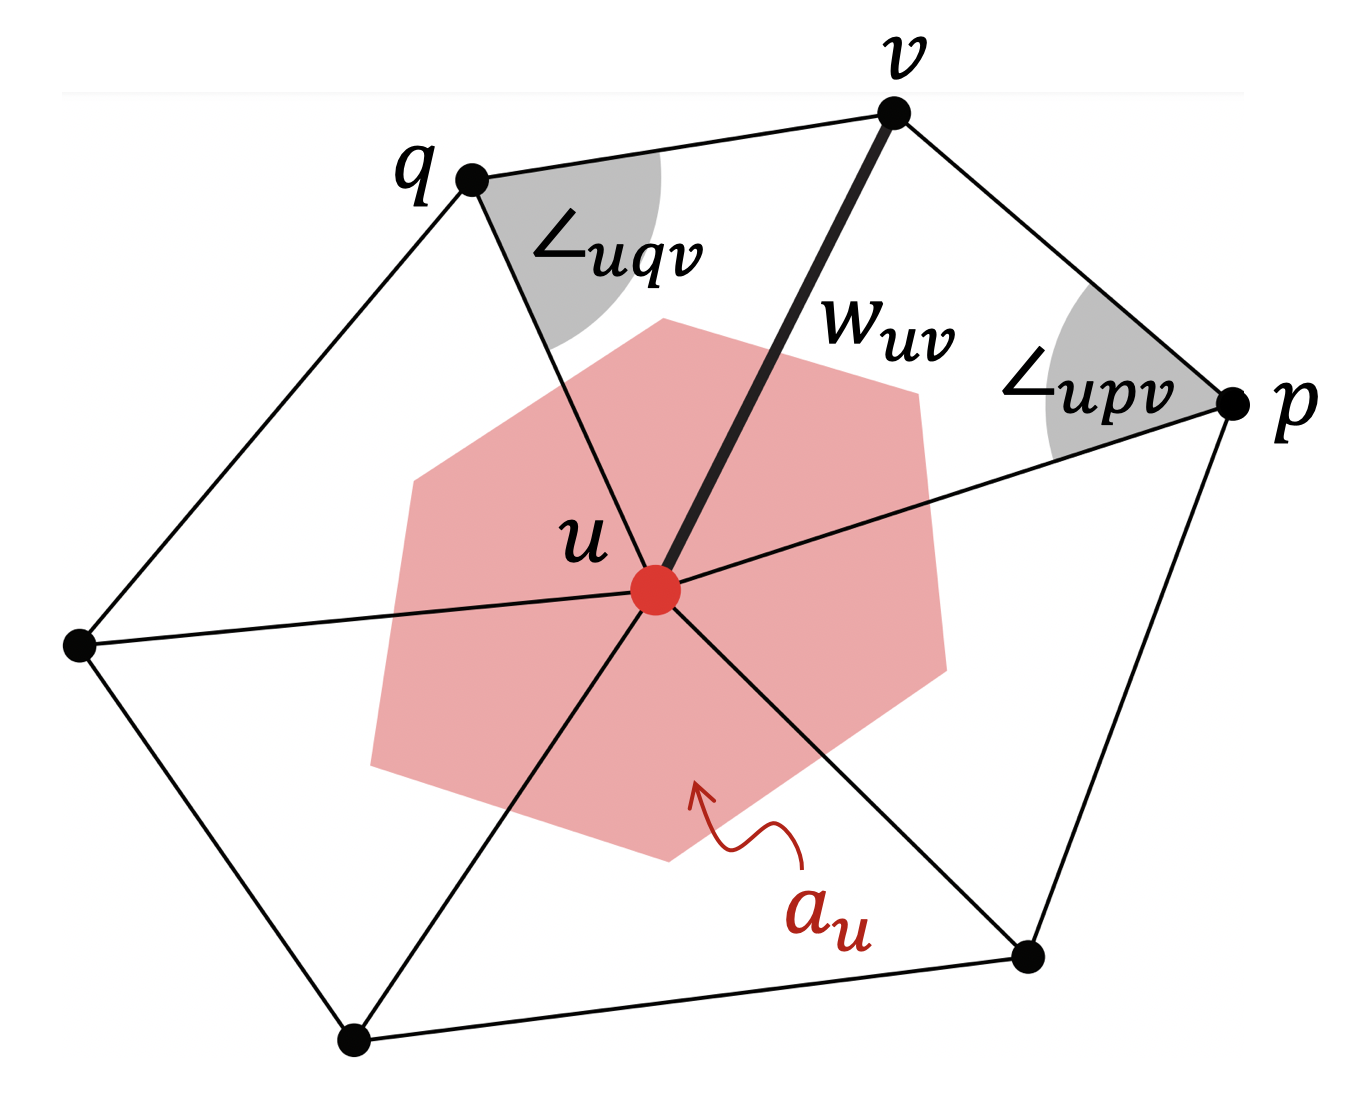
\includegraphics[width=\linewidth]{figures/cotan.png}
这一公式最早见于 \cite{macneal1949solution} 的博士论文；他提出该公式是为了在 Caltech Electric Analog Computer 上求解 PDE。}
\begin{equation}
w_{uv} = \frac{\cot \angle_{uqv} + \cot \angle_{upv}}{2 a_u}
\label{eq:cotan}
\end{equation}
其中，$\angle_{uqv}$ 和 $\angle_{upv}$ 分别是三角形 $(u,q,v)$ 与 $(u,p,v)$ 中共享边 $(u,v)$ 所对的两个角；$a_u$ 是局部面积元，通常计算为由三角形 $(u,p,q)$（它们共享节点 $u$）的重心所构成多边形的面积，即
%
$a_u = \frac{1}{3}\sum_{v,q : (u,v,q) \in \mathcal{F}} a_{uvq}$.


可以证明，余切 Laplacian 具有多种便利性质（例如见 \cite{wardetzky2007discrete}）：它是{\em 半正定}矩阵，$\boldsymbol{\Delta} \succcurlyeq 0$，因而具有可视作频率类比的非负特征值 $\lambda_1 \leq \hdots \leq \lambda_n$；它是对称的，因而具有正交特征向量；并且它是{\em 局部的}（即 $(\boldsymbol{\Delta}\mathbf{X})_u$ 的值只依赖一跳邻居 $\mathcal{N}_u$）。
%
也许最重要的性质是：当网格曲面被无限细化时，余切网格 Laplacian 矩阵 $\boldsymbol{\Delta}$ 收敛于连续算子 $\Delta$ \citep{wardetzky2008convergence}。因此，式~（\ref{eq:cotan}）构成了第~\ref{sec:manifolds} 节所定义 Riemann 流形上 Laplacian 算子的一种恰当{\em 离散化}\marginnote{必须对细化施加一些技术条件，以避免三角形变得病态等情况。一个例子是圆柱面的一种奇异三角剖分，在德文中称为 {\em Schwarzscher Stiefel}（Schwarz's boot），在英文文献中称为 ``Schwarz lantern''；它由因 Cauchy--Schwarz 不等式而闻名的德国数学家 Hermann Schwarz 于 1880 年提出。}。


尽管人们预期 Laplacian 是内蕴的，但这一点从式~（\ref{eq:cotan}）看并不明显；需要经过一些推导，才能将余切权重完全用离散度量 $\ell$ 表示为
$$
w_{uv} = \frac{-\ell^2_{uv} + \ell^2_{vq} + \ell^2_{uq} }{8 a_{uvq}} + 
\frac{-\ell^2_{uv} + \ell^2_{vp} + \ell^2_{up} }{8 a_{uvp}}
$$
%
其中，三角形面积 $a_{ijk}$ 为
$$
a_{uvq} = \sqrt{s_{uvq} (s_{uvq} - \ell_{uv}) (s_{uvq} - \ell_{vq}) (s_{uvq} - \ell_{uq}) }
$$
这里采用{\em Heron 半周长公式}，其中
%$s_{ijk} = \frac{1}{2}(\ell_{ij} + \ell_{ik} + \ell_{jk})$. 
$s_{uvq} = \frac{1}{2}(\ell_{uv} + \ell_{uq} + \ell_{vq})$. 
%
%
这使 Laplacian（以及与之相关的任何量，如其特征向量和特征值）具有{\em 等距不变性}；正因如此，它在几何处理和计算机图形学中备受青睐（见 \cite{wang2019intrinsic} 的优秀综述）：任何不影响度量 $\ell$ 的网格曲面形变（即不“拉伸”或“压缩”网格边）都不会改变 Laplacian。



最后，正如我们已经注意到的，\marginnote{
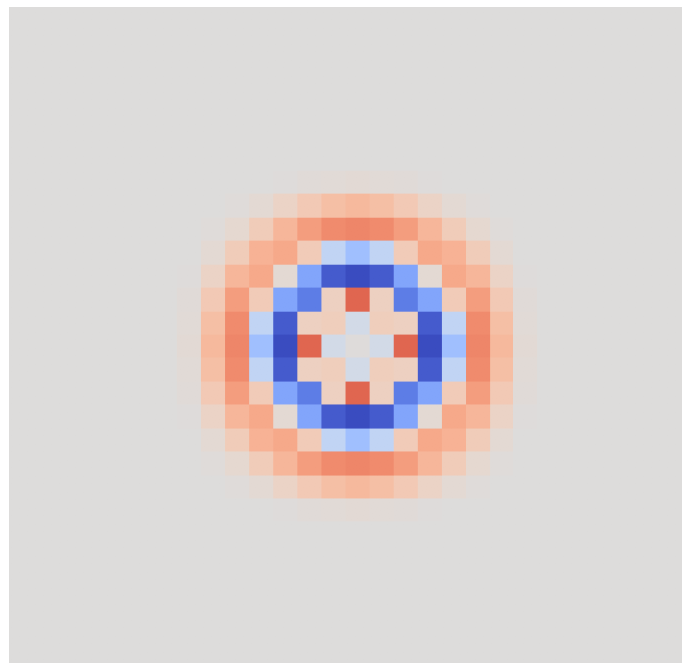
\includegraphics[width=0.9\linewidth]{figures/isotropic.png}
基于 Laplacian 的滤波器是各向同性的。在平面上，这类滤波器具有径向对称性。
} Laplacian 的定义~（\ref{eq:cotan}）对于 $\mathcal{N}_u$ 中节点的置换保持不变，因为它采用了求和形式的聚合。
%
在一般图上，由于邻居缺少规范排序，这是一种不得不接受的限制；而在网格曲面上，可以按照某种定向（例如顺时针）排列一跳邻居，唯一的歧义在于第一个节点的选择。因此，我们无须考虑任意可能的置换，而只需考虑{\em 循环移位}（旋转）；直观地说，这对应于第~\ref{sec:gauges} 节讨论的 $\mathrm{SO}(2)$ 规范变换所产生的歧义。
%
对于固定规范，可以定义对局部方向敏感的{\em 各向异性 Laplacian}；这等价于改变度量或权重 $w_{uv}$。
%
\cite{andreux2014anisotropic,boscaini2016anisotropic} 曾用此类构造设计形状描述符，\cite{boscaini2016learning} 也将其用于早期的网格曲面几何深度学习架构。



\paragraph{网格曲面上的谱分析}
%
将 Laplacian 矩阵对角化的正交特征向量\linebreak[4] $\boldsymbol{\Phi} = (\boldsymbol{\varphi}_1, \hdots, \boldsymbol{\varphi}_n)$（$\boldsymbol{\Delta} = \boldsymbol{\Phi} \boldsymbol{\Lambda} \boldsymbol{\Phi}^\top$，其中 $\boldsymbol{\Lambda} = \mathrm{diag}(\lambda_1, \hdots, \lambda_n)$ 是 Laplacian 特征值的对角矩阵）可用作 Fourier 基的非 Euclidean 类比，从而能把相应 Fourier 变换的乘积作为网格曲面上的谱卷积：
$$
\mathbf{X} \star \boldsymbol{\theta} = 
\boldsymbol{\Phi} \, \mathrm{diag}(\boldsymbol{\Phi}^\top \boldsymbol{\theta}) (\boldsymbol{\Phi}^\top \mathbf{X}) 
=
\boldsymbol{\Phi}\, \mathrm{diag}(\hat{\boldsymbol{\theta}}) \hat{\mathbf{X}},
$$
%
其中，滤波器 $\hat{\boldsymbol{\theta}}$ 直接在 Fourier 域中设计。
%
同样，这个公式中没有任何网格曲面特有的内容，也可以使用一般（无向）图的 Laplacian 矩阵。\marginnote{图为无向图这一假设很重要：此时 Laplacian 是对称的，并具有正交特征向量。}
%
%
利用卷积的这一谱定义把 CNN 推广到图上是一个很自然的想法；事实上，本文的一位作者已在 \cite{bruna2013spectral} 中这样做过。
%
然而，非 Euclidean Fourier 变换似乎
对底层网格曲面或图的微小扰动也极为敏感（见第~\ref{sec:manifolds} 节的图~\ref{fig:mesh_horses}），因此它只能用于处理{\em 固定}域上的不同信号，而不能用于在{\em 不同域}之间泛化。
%
遗憾的是，许多计算机图形学与视觉问题都属于后一类：神经网络在一组 3D 形状（网格曲面）上训练，却在另一组形状上测试，因而基于 Fourier 变换的方法并不适用。

%is given a training set of 3D shapes (meshes) and a different test, the generalisation across domains 



正如第~\ref{sec:manifolds} 节所指出的，更可取的做法是使用形如~（\ref{eqn:conv_spec}）的谱滤波器，即把某个传递函数 $\hat{p}(\lambda)$ 应用于 Laplacian 矩阵：
$$
\hat{p}(\boldsymbol{\Delta})\mathbf{X} = \boldsymbol{\Phi} \hat{p}(\boldsymbol{\Lambda})\boldsymbol{\Phi}^\top\mathbf{X} 
= \boldsymbol{\Phi}\, \mathrm{diag}(\hat{p}(\lambda_1), \hdots, \hat{p}(\lambda_n)) \hat{\mathbf{X}}. 
$$
%
%which can be parametrised with a small number of parameters and computer efficiently. 
%
当 $\hat{p}$ 可以用矩阵--向量乘积表示时，就可以完全避免对 $n\times n$ 矩阵 $\boldsymbol{\Delta}$ 进行特征分解。\marginnote{一般情况下，特征分解的复杂度为 $\mathcal{O}(n^3)$。}
%
例如，\cite{defferrard2016convolutional} 使用 $r$ 次{\em 多项式}作为滤波函数，%in which case the filter is expressed as
$$
\hat{p}(\boldsymbol{\Delta})\mathbf{X} = \sum_{k=0}^r \alpha_k \boldsymbol{\Delta}^k \mathbf{X}  = \alpha_0 \mathbf{X} + \alpha_1 \boldsymbol{\Delta} \mathbf{X}  + \hdots + \alpha_r \boldsymbol{\Delta}^r \mathbf{X}, 
$$
这相当于把 $n\times d$ 特征矩阵 $\mathbf{X}$ 与 $n\times n$ Laplacian 矩阵相乘 $r$ 次。由于 Laplacian 通常是稀疏的（具有 $\mathcal{O}(|\mathcal{E}|)$ 个非零元素），\marginnote{网格曲面是近正则图，每个节点具有 $\mathcal{O}(1)$ 个邻居，因此有 $\mathcal{O}(n)$ 个非零元素位于 $\boldsymbol{\Delta}$ 中。}
%
该运算具有较低的复杂度 $\mathcal{O}(|\mathcal{E}|dr)\sim \mathcal{O}(|\mathcal{E}|)$。
%
此外，由于 Laplacian 是局部的，%(i.e., the value of $(\boldsymbol{\Delta}\mathbf{X})_i$ depends only on 1-hop neighbours, $\mathcal{N}_i$),
$r$ 次多项式滤波器局部化在 $r$ 跳邻域内。


然而，在处理网格曲面时，这一精确性质会带来不利之处，因为滤波器的实际支撑（即其覆盖半径）取决于网格曲面的{\em 分辨率}。
%
必须牢记，网格曲面来自某个底层连续曲面的离散化，因此两个不同网格曲面 $\mathcal{T}$ 和 $\mathcal{T}'$ 可能表示{\em 同一个对象}。\marginnote{    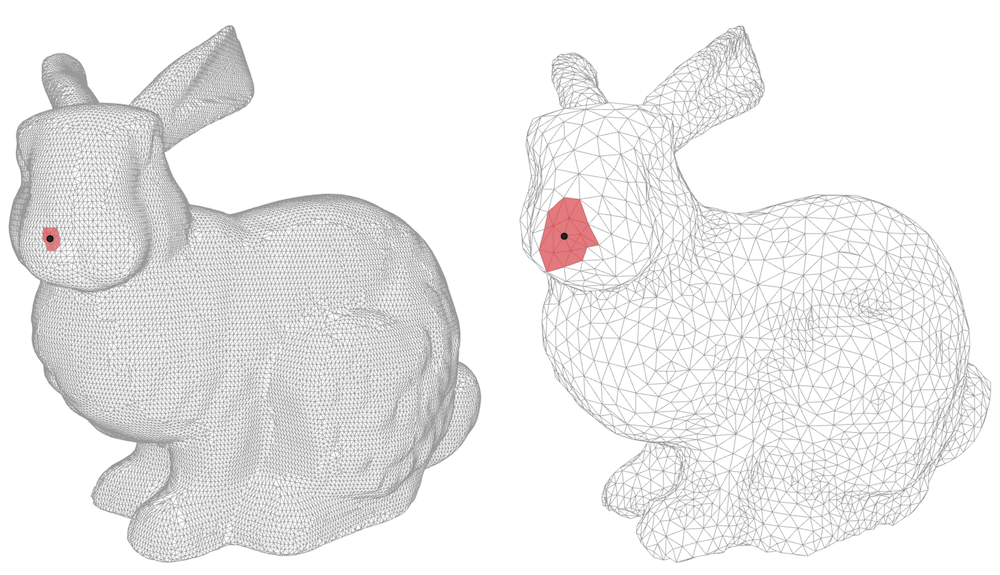
\includegraphics[width=\linewidth]{figures/mesh_res.png}\\
不同分辨率网格曲面上的两跳邻域。}
%
在较细网格曲面上，可能必须使用比粗网格曲面更大的邻域（因而滤波器的次数 $r$ 也更高）。
%

因此，计算机图形学应用中更常使用{\em 有理滤波器}，因为它们与分辨率无关。这类滤波器有多种定义方式（例如见 \cite{patane2020fourier}），最常见的是取某个有理函数（例如 $\frac{\lambda-1}{\lambda+1}$）的多项式。
%
更一般地，可以使用复函数，例如把实直线映射到复平面单位圆上的{\em Cayley 变换} $\frac{\lambda - \mi}{ \lambda + \mi}$。\marginnote{Cayley 变换是 {\em M{\"o}bius 变换}的一种特殊情形。将其作用于 Laplacian（一个半正定矩阵）时，它会把非负特征值映射到复半圆上。}
%
\cite{levie2018cayleynets} 使用表示为{\em Cayley 多项式}的谱滤波器，即具有复系数 $\alpha_l \in \mathbb{C}$ 的实值有理函数：
$$
\hat{p}(\lambda) = \mathrm{Re} \left(  \sum_{l=0}^r 
\alpha_l \left( \frac{\lambda - \mi}{ \lambda + \mi}
\right)^{l}
\right).
$$
%
将 Cayley 多项式应用于矩阵时，其计算需要矩阵求逆：
$$
\hat{p}(\boldsymbol{\Delta}) = \mathrm{Re} \left(  \sum_{l=0}^r
\alpha_l (\boldsymbol{\Delta} - \mi\mathbf{I})^{l} (\boldsymbol{\Delta} + \mi\mathbf{I})^{-l}
\right),\marginnote{In signal processing, polynomial filters are termed {\em finite impulse response} (FIR), whereas rational filters are {\em infinite impulse response} (IIR).}
$$
这一计算可以用线性复杂度近似完成。
%
与多项式滤波器不同，有理滤波器不具有局部支撑，但会指数衰减，%and thus localised
\citep{levie2018cayleynets}.  
%
与直接计算 Fourier 变换相比，一个关键区别在于，多项式滤波器和有理滤波器在底层图或网格曲面的近似等距形变下是稳定的——例如，\cite{levie2018cayleynets,levie2019transferability,gama2020stability,kenlay2021interpretable} 给出了多种此类结果。



%\paragraph{Anisotropic Laplacians}






\paragraph{作为算子的网格曲面与函数映射}


函数映射范式启发我们把网格曲面视为{\em 算子}。如下文所示，这使我们能够利用网格曲面的附加结构，得到更丰富的不变性类型。
%
为便于讨论，假定网格曲面 $\mathcal{T}$ 由坐标为 $\mathbf{X}$ 的嵌入节点构成。
%
如果构造 Laplacian 这样的内蕴算子，可以证明它完整编码了网格曲面的结构，并且能够恢复该网格曲面（精确到其等距嵌入，见 \cite{zeng2012discrete}）。
%
某些其他算子也具有这一性质（例如见 \cite{boscaini2015shape,corman2017functional,chern2018shape}），因此我们将用一般算子，即 $n\times n$ 矩阵 $\mathbf{Q}(\mathcal{T}, \mathbf{X})$，表示网格曲面。


从这一视角看，第~\ref{sec:proto-graphs} 节关于学习形如 $f(\mathbf{X},\mathcal{T})$ 的函数的讨论，%(as we had in our discussion on graphs in Section~\ref{sec:proto-graphs})
可以重新表述为
学习形如 $f(\mathbf{Q})$ 的函数。
%
与图和集合类似，网格曲面的节点同样没有规范排序；也就是说，网格曲面上的函数必须满足置换不变或置换等变条件：
\begin{eqnarray*}
f(\mathbf{Q}) &=& f(\mathbf{P}\mathbf{Q}\mathbf{P}^\top) \\
%
\mathbf{P}\mathbf{F}(\mathbf{Q}) &=& \mathbf{F}(\mathbf{P}\mathbf{Q}\mathbf{P}^\top)
\end{eqnarray*}
% 
上述关系对任意置换矩阵 $\mathbf{P}$ 都成立。
%Conceptually, the permutation matrix can be considered as {\em correspondence} between two isomorphic meshes, i.e., meshes with the same number of nodes and identical connectivity. 
%
%
不过，与一般图相比，这里具有更多结构：可以假定网格曲面来自某个底层连续曲面 $\Omega$ 的离散化。因此，另一个网格曲面 $\mathcal{T}'=(\mathcal{V}',\mathcal{E}',\mathcal{F}')$ 可以由 $n'$ 个节点及其坐标 $\mathbf{X}'$ 构成；它所表示的对象 $\Omega$ 与 $\mathcal{T}$ 所表示的相同。
%\marginnote{It is convenient to think of $\mathcal{T}'$ as a {\em remeshing} of $\mathcal{T}$.}  
%
%
重要的是，网格曲面 $\mathcal{T}$ 和 $\mathcal{T}'$ 可以具有不同的连通结构，甚至具有不同的节点数（$n'\neq n$）。因此，不能把这些网格曲面视为仅仅重新排列了节点的同构图，也不能把置换矩阵 $\mathbf{P}$ 视为二者之间的对应关系。


\cite{ovsjanikov2012functional} 引入了函数映射，把对应关系的概念推广到这类情形：它用{\em 函数}之间的对应关系，取代两个域上{\em 点}之间的对应关系（映射 $\eta : \Omega \rightarrow \Omega'$）；前者由映射 $\mathbf{C}:\mathcal{X}(\Omega) \rightarrow \mathcal{X}(\Omega')$ 给出，见图~\ref{fig:func_maps}。
%
{\em 函数映射}是一个线性算子
$\mathbf{C}$，表示为 $n'\times n$ 矩阵，用于在信号 $\mathbf{x}'$
%\in \mathcal{X}(\mathcal{T}')$  
%defined on the nodes of the mesh of $\mathcal{T}'$ 
与 $\mathbf{x}$ % \in \mathcal{X}(\mathcal{T})$ as
各自所在的域之间建立如下对应关系：
%defined on the nodes of the mesh of $\mathcal{T}$ as 
$$
\mathbf{x}' = \mathbf{C}\mathbf{x}.\marginnote{
In most cases the functional map is implemented in the spectral domain, as a $k\times k$ map $\hat{\mathbf{C}}$ between the Fourier coefficients,
$
\mathbf{x}' = \boldsymbol{\Phi}'\hat{\mathbf{C}}\boldsymbol{\Phi}^\top\mathbf{x},
$
where $\boldsymbol{\Phi}$ and $\boldsymbol{\Phi}'$ are the respective $n\times k$ and $n'\times k$ matrices of the (truncated) Laplacian eigenbases, with $k\ll n,n'$. 
}
$$
%
%
%\michael{[TODO: Typically, $C$ is constructed in the Fourier domain - explain how. We want to have $C$ square to avoid problems with dimensions]}
\cite{rustamov2013map} 证明，为保证映射{\em 保面积}，函数映射必须正交，即 $\mathbf{C}^\top \mathbf{C} = \mathbf{I}$；换言之，它必须是正交群的一个元素 $\mathbf{C} \in \mathrm{O}(n)$。此时，可以用 $\mathbf{C}^{-1} = \mathbf{C}^\top$ 对该映射求逆。


\begin{figure}[h!]
    \centering
    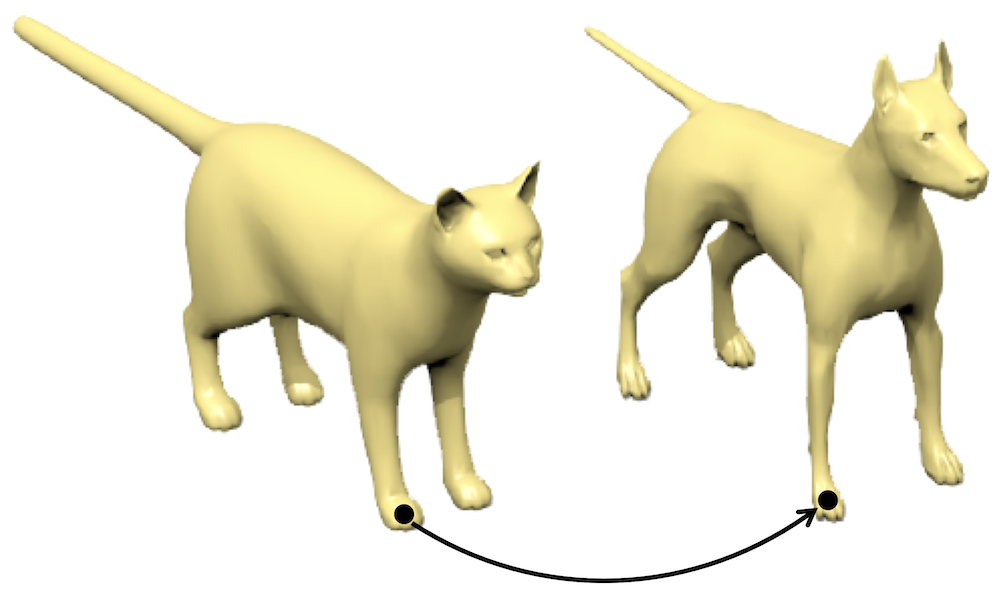
\includegraphics[width=0.45\linewidth]{figures/map_point.png}\hspace{5mm}    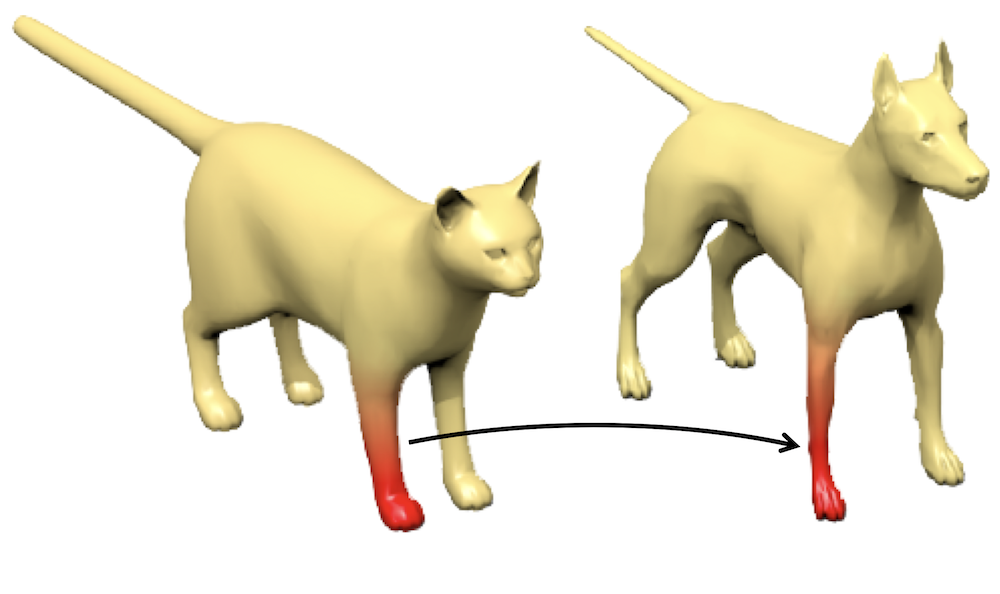
\includegraphics[width=0.45\linewidth]{figures/map_func.png}
    \caption{逐点映射（左）与函数映射（右）。
    }
    \label{fig:func_maps}
\end{figure}%


函数映射还在网格曲面的算子表示之间建立了如下关系：
$$
\mathbf{Q}' = \mathbf{C} \mathbf{Q} \mathbf{C}^\top, \quad \quad \mathbf{Q} = \mathbf{C}^\top \mathbf{Q}' \mathbf{C}, 
$$
%
可以作如下解释：给定算子表示 $\mathbf{Q}$（对应于 $\mathcal{T}$）和函数映射 $\mathbf{C}$，可以构造表示 $\mathbf{Q}'$（对应于 $\mathcal{T}'$）；具体而言，先把信号从 $\mathcal{T}'$ 映射到 $\mathcal{T}$（使用 $\mathbf{C}^\top$），再应用算子 $\mathbf{Q}$，最后映射回 $\mathcal{T}'$（使用 $\mathbf{C}$）。\marginnote{请注意，这些运算按\emph{从右到左}的顺序读取。}
%, i.e. we assume left-multiplication with a signal on $\mathcal{T}'$.}. 
%
由此得到一类更一般的网格曲面上的{\em 重网格化不变}（或等变）函数，它们满足
%
\begin{eqnarray*}
f(\mathbf{Q}) &=& f(\mathbf{C}\mathbf{Q}\mathbf{C}^\top) = f(\mathbf{Q}')\\
%
\mathbf{C}\mathbf{F}(\mathbf{Q}) &=& \mathbf{F}(\mathbf{C}\mathbf{Q}\mathbf{C}^\top) = \mathbf{F}(\mathbf{Q}')
\end{eqnarray*}
% 
上述关系对任意 $\mathbf{C} \in \mathrm{O}(n)$ 都成立。
%
不难看出，前述置换不变性与置换等变性的设定是一个特殊情形；\marginnote{这源于置换矩阵的正交性，即 $\mathbf{P}^\top \mathbf{P} = \mathbf{I}$。}
它可以看作一种只改变节点顺序的平凡重网格化。


\cite{wang2019learning} 证明，给定算子 $\mathbf{Q} = \mathbf{V}\boldsymbol{\Lambda}\mathbf{V}^\top$ 的特征分解，任意重网格化不变（或等变）函数都可以表示为
%
%
$f(\mathbf{Q}) = f(\boldsymbol{\Lambda})$，以及
%
$\mathbf{F}(\mathbf{Q}) = \mathbf{V} \mathbf{F}(\boldsymbol{\Lambda})$, 
%
换言之，重网格化不变函数{\em 仅涉及} $\mathbf{Q}$ {\em 的谱}。
%
%
实践已经证明，Laplacian 特征值的函数对于曲面离散化和扰动具有鲁棒性；这解释了基于 Laplacian 的谱构造为何在计算机图形学以及图深度学习中广受欢迎 \citep{defferrard2016convolutional,levie2018cayleynets}。
%
%In graph deep learning literature, architectures such as ChebNet \citep{defferrard2016convolutional} and CayleyNet \citep{levie2018cayleynets} explicitly learn functions of Laplacian eigenvalues. 
%
%
由于这一结果适用于一般算子 $\mathbf{Q}$，除了无处不在的 Laplacian 之外，还有多种选择——值得注意的例子包括 Dirac 算子 \citep{liu2017dirac,kostrikov2018surface}、Steklov 算子 \citep{wang2018steklov}，以及可学习的参数化算子 \citep{wang2019learning}。


%\michael{The degree of freedom we have is the operator itself - which leads to learnable operators.}

%\joan{We might want to mention extrinsic models that build anisotropy based on the Dirac Operator rather than the Laplace operator; Crane et al, and our Surface Network paper}
%\joan{This section clearly needs to branch out into its own chapter. }
